\documentclass[a4paper,11pt]{book}
%\documentclass[a4paper,twoside,11pt,titlepage]{book}
\usepackage{listings}
\usepackage[utf8]{inputenc}
\usepackage[spanish]{babel}
\usepackage{float}

% \usepackage[style=list, number=none]{glossary} %
%\usepackage{titlesec}
%\usepackage{pailatino}

\decimalpoint
\usepackage{dcolumn}
\newcolumntype{.}{D{.}{\esperiod}{-1}}
\makeatletter
\addto\shorthandsspanish{\let\esperiod\es@period@code}
\makeatother


%\usepackage[chapter]{algorithm}
\RequirePackage{verbatim}
%\RequirePackage[Glenn]{fncychap}
\usepackage{fancyhdr}
\usepackage{graphicx}
\usepackage{afterpage}
\usepackage{array}
\usepackage{makecell}
\usepackage{tabularray}
\usepackage{vcell}
\usepackage{booktabs}
\usepackage{textgreek}
\usepackage{amsmath} %Para poder usar \being{equation*}
\usepackage[gen]{eurosym} %Para usar el simbolo del euro en entornos varios 
\usepackage{rotating}
\usepackage[export]{adjustbox}

\usepackage{longtable}

\usepackage[pdfborder={000}]{hyperref} %referencia

\usepackage[backend=biber, style=numeric, sorting=ynt]{biblatex}


% \usepackage{booktabs}
% \usepackage{dirtree}
% \usepackage{algorithmicx}
% \usepackage{algorithm}
\usepackage[font=small, margin=0.1cm]{caption}
% \usepackage{subcaption}
\usepackage{multirow}
% \usepackage{enumitem}
% \setlist{nosep}

\newcommand{\INDSTATE}[1][1]{\STATE\hspace{#1\algorithmicindent}}

% \usepackage[
%     a4paper,
%     left=2.8cm,
%     right=2.7cm,
%     top=4cm,
%     bottom=3cm
% ]{geometry}

% ********************************************************************
% Re-usable information
% ********************************************************************
\newcommand{\myTitle}{Detección de errores en bases de datos químicas\xspace}
\newcommand{\myDegree}{Grado en Ingeniería Informática\xspace}
\newcommand{\myName}{Jesús Navarro Merino\xspace}
\newcommand{\myProf}{Rocío Celeste Romero Zaliz\xspace}
%\newcommand{\mySupervisor}{Put name here\xspace}
\newcommand{\myFaculty}{Escuela Técnica Superior de Ingenierías Informática y de
Telecomunicación\xspace}
\newcommand{\myFacultyShort}{E.T.S. de Ingenierías Informática y de
Telecomunicación\xspace}
\newcommand{\myDepartment}{Departamento de ...\xspace}
\newcommand{\myUni}{\protect{Universidad de Granada}\xspace}
\newcommand{\myLocation}{Granada\xspace}
\newcommand{\myTime}{\today\xspace}
\newcommand{\myVersion}{Version 0.1\xspace}


\hypersetup{
pdfauthor = {\myName (email (en) ugr (punto) es)},
pdftitle = {\myTitle},
pdfsubject = {},
pdfkeywords = {palabra_clave1, palabra_clave2, palabra_clave3, ...},
pdfcreator = {LaTeX con el paquete ....},
pdfproducer = {pdflatex}
}

%\hyphenation{}


%\usepackage{doxygen/doxygen}
%\usepackage{pdfpages}
\usepackage{url}
\usepackage{color,colortbl,longtable}
\usepackage{tabularx}
\usepackage{lscape}
\usepackage[stable]{footmisc}
\usepackage{subcaption}
\usepackage{dirtree}
%\usepackage{index}

%\makeindex
%\usepackage[style=long, cols=2,border=plain,toc=true,number=none]{glossary}
% \makeglossary

% Definición de comandos que me son tiles:
%\renewcommand{\indexname}{Índice alfabético}
%\renewcommand{\glossaryname}{Glosario}

\pagestyle{fancy}
\fancyhf{}
\fancyhead[LO]{\leftmark}
\fancyhead[RE]{\rightmark}
\fancyhead[RO,LE]{\textbf{\thepage}}
\renewcommand{\chaptermark}[1]{\markboth{\textbf{#1}}{}}
\renewcommand{\sectionmark}[1]{\markright{\textbf{\thesection. #1}}}

\setlength{\headheight}{1.5\headheight}

\newcommand{\HRule}{\rule{\linewidth}{0.5mm}}
%Definimos los tipos teorema, ejemplo y definición podremos usar estos tipos
%simplemente poniendo \begin{teorema} \end{teorema} ...
\newtheorem{teorema}{Teorema}[chapter]
\newtheorem{ejemplo}{Ejemplo}[chapter]
\newtheorem{definicion}{Definición}[chapter]

\definecolor{gray97}{gray}{.97}
\definecolor{gray75}{gray}{.75}
\definecolor{gray45}{gray}{.45}
\definecolor{gray30}{gray}{.94}

\lstset{ frame=none,
     framerule=0.5pt,
     aboveskip=0.5cm,
     framextopmargin=3pt,
     framexbottommargin=3pt,
     framexleftmargin=0.1cm,
     framesep=0pt,
     rulesep=.4pt,
     backgroundcolor=\color{gray97},
     rulesepcolor=\color{black},
     %
     stringstyle=\ttfamily,
     showstringspaces = false,
     basicstyle=\scriptsize\ttfamily,
     commentstyle=\color{gray45},
     keywordstyle=\bfseries,
     %
     numbers=none,
     numbersep=6pt,
     numberstyle=\tiny,
     numberfirstline = false,
     breaklines=true,
   }

    % Añadir algunos caracteres especiales para manejar utf-8 con lstlisting
   \lstset{literate=
  {á}{{\'a}}1 {é}{{\'e}}1 {í}{{\'i}}1 {ó}{{\'o}}1 {ú}{{\'u}}1
  {Á}{{\'A}}1 {É}{{\'E}}1 {Í}{{\'I}}1 {Ó}{{\'O}}1 {Ú}{{\'U}}1
  {à}{{\`a}}1 {è}{{\`e}}1 {ì}{{\`i}}1 {ò}{{\`o}}1 {ù}{{\`u}}1
  {À}{{\`A}}1 {È}{{\`E}}1 {Ì}{{\`I}}1 {Ò}{{\`O}}1 {Ù}{{\`U}}1
  {ä}{{\"a}}1 {ë}{{\"e}}1 {ï}{{\"i}}1 {ö}{{\"o}}1 {ü}{{\"u}}1
  {Ä}{{\"A}}1 {Ë}{{\"E}}1 {Ï}{{\"I}}1 {Ö}{{\"O}}1 {Ü}{{\"U}}1
  {â}{{\^a}}1 {ê}{{\^e}}1 {î}{{\^i}}1 {ô}{{\^o}}1 {û}{{\^u}}1
  {Â}{{\^A}}1 {Ê}{{\^E}}1 {Î}{{\^I}}1 {Ô}{{\^O}}1 {Û}{{\^U}}1
  {ã}{{\~a}}1 {ẽ}{{\~e}}1 {ĩ}{{\~i}}1 {õ}{{\~o}}1 {ũ}{{\~u}}1
  {Ã}{{\~A}}1 {Ẽ}{{\~E}}1 {Ĩ}{{\~I}}1 {Õ}{{\~O}}1 {Ũ}{{\~U}}1
  {œ}{{\oe}}1 {Œ}{{\OE}}1 {æ}{{\ae}}1 {Æ}{{\AE}}1 {ß}{{\ss}}1
  {ű}{{\H{u}}}1 {Ű}{{\H{U}}}1 {ő}{{\H{o}}}1 {Ő}{{\H{O}}}1
  {ç}{{\c c}}1 {Ç}{{\c C}}1 {ø}{{\o}}1 {Ø}{{\O}}1 {å}{{\r a}}1 {Å}{{\r A}}1
  {€}{{\euro}}1 {£}{{\pounds}}1 {«}{{\guillemotleft}}1
  {»}{{\guillemotright}}1 {ñ}{{\~n}}1 {Ñ}{{\~N}}1 {¿}{{?`}}1 {¡}{{!`}}1 
}
 
% minimizar fragmentado de listados
\lstnewenvironment{listing}[1][]
   {\lstset{#1}\pagebreak[0]}{\pagebreak[0]}

\lstdefinestyle{CodigoC}
   {
	basicstyle=\scriptsize,
	frame=none,
	language=C,
	numbers=left
   }
\lstdefinestyle{CodigoC++}
   {
	basicstyle=\small,
	frame=none,
	backgroundcolor=\color{gray30},
	language=C++,
	numbers=left
   }

 
\lstdefinestyle{Consola}
   {basicstyle=\scriptsize\bf\ttfamily,
    backgroundcolor=\color{gray30},
    frame=none,
    numbers=none
   }


\newcommand{\bigrule}{\titlerule[0.5mm]}
\newcommand{\footnotecomma}{$^{,}$}

%Para conseguir que en las páginas en blanco no ponga cabecerass
\makeatletter
\def\clearpage{%
  \ifvmode
    \ifnum \@dbltopnum =\m@ne
      \ifdim \pagetotal <\topskip
        \hbox{}
      \fi
    \fi
  \fi
  \newpage
  \thispagestyle{empty}
  \write\m@ne{}
  \vbox{}
  \penalty -\@Mi
}
\makeatother

\usepackage{pdfpages}


\addbibresource{bibliografia/bibliografia.bib}
% \addbibresource{sample.bib}
% \addbibresource{bibliografia/webs.bib}

\begin{document}
\begin{titlepage}
 
 
\newlength{\centeroffset}
\setlength{\centeroffset}{-0.5\oddsidemargin}
\addtolength{\centeroffset}{0.5\evensidemargin}
\thispagestyle{empty}

\noindent\hspace*{\centeroffset}\begin{minipage}{\textwidth}

\centering

\includegraphics[width=0.9\textwidth]{imagenes/logos/logo_ugr.jpg}\\[1.4cm]

\textsc{ \Large TRABAJO FIN DE GRADO\\[0.2cm]}
\textsc{ INGENIERÍA INFORMÁTICA}\\[1cm]
% Upper part of the page
% 
% Title
\noindent\rule[-1ex]{\textwidth}{2pt}\\[3ex]
{\Huge\bfseries Prueba Detección de errores en bases de datos químicas\\
}
\noindent\rule[-3ex]{\textwidth}{2pt}\\[3ex]
\end{minipage}

\vspace{1.5cm}
\noindent\hspace*{\centeroffset}\begin{minipage}{\textwidth}
\centering

\textbf{Autor}\\ {Jesús Navarro Merino}\\[2.5ex]
\textbf{Directora}\\
{Rocío Celeste Romero Zaliz}\\[2cm]

\includegraphics[width=0.3\textwidth]{imagenes/logos/etsiit_logo.png}\\[0.1cm]
\textsc{Escuela Técnica Superior de Ingenierías Informática y de Telecomunicación}\\
\textsc{---}\\
Granada, julio de 2023
\end{minipage}
%\addtolength{\textwidth}{\centeroffset}
%\vspace{\stretch{2}}
\end{titlepage}


\chapter*{}
%\thispagestyle{empty}
%\cleardoublepage

%\thispagestyle{empty}


% \cleardoublepage
\thispagestyle{empty}

\begin{center}
{\large\bfseries Detección de errores en bases de datos químicas}\\
\end{center}
\begin{center}
Jesús Navarro Merino\\
\end{center}

%\vspace{0.7cm}
\noindent{\textbf{Palabras clave}: Química computacional, Química organometálica, Nomenclatura canónica, SMILES, Representación de moléculas, Cp, OpenBabel, Bases de datos, SciFinder.}\\

\vspace{0.7cm}
\noindent{\textbf{Resumen}}\\

El desarrollo de la informática y la aplicación de sus métodos al mundo de la química ha propiciado grandes avances en esta ciencia. Sin embargo, un campo poco explorado dentro de la química computacional es la organometálica, de manera que muchas de las herramientas existentes no están preparadas para trabajar con ella. En esta área, para los investigadores es importante codificar las moléculas en representaciones lineales como SMILES y usar las herramientas software, para entre otras cosas, representar los compuestos gráficamente y comprenderlos mejor. La heterogeneidad en las distintas bases de datos públicas a la hora de consultar un mismo compuesto entorpece el trabajo de los investigadores.

Tras un análisis de esas inconsistencias, este proyecto propone una nomenclatura canónica para moléculas organometálicas en donde se le dé la suficiente importancia al metal, de manera que quede colocado el primero en el SMILES canónico resultado. En química de coordinación y organometálica, las reacciones y los compuestos no se explican bien siguiendo la teoría del enlace de valencia. Por tanto, se presentan también algunos cambios en el sistema de representación 2D de la herramienta utilizada, para ilustrar de una manera más adecuada los enlaces metal-ligando más habituales en compuestos organometálicos, las estructuras de ciclopentadienilo (Cp). Tras la validación de los resultados con diversos tests de consistencia, se obtienen finalmente resultados satisfactorios.

\cleardoublepage


\thispagestyle{empty}


\begin{center}
{\large\bfseries Error detection in chemical databases}\\
\end{center}
\begin{center}
Jesús Navarro Merino\\
\end{center}

%\vspace{0.7cm}
\noindent{\textbf{Keywords}: Chemoinformatics, Organometallic chemistry, Canonicalization, SMILES, Molecule depiction, Cp, OpenBabel, Databases, SciFinder.}\\

\vspace{0.7cm}
\noindent{\textbf{Abstract}}\\

The development of computer science and the application of its methods to the chemical world has led to great advances in this science. However, a less explored field within computational chemistry is organometallics, meaning that many of the existing tools are not prepared to work with it. In this area, it is important for researchers to encode molecules in linear notations such as SMILES and use software tools to, among other things, depict compounds graphically and have a better understanding of them. Heterogeneity in various public databases when querying the same compound hinders scientists' work.

After an analysis of these inconsistencies, this project proposes a canonical nomenclature for organometallic molecules in which adequate importance is given to the metal, so that it is placed first in the resulting canonical SMILES. In coordination and organometallic chemistry, reactions and compounds do not fit well into the valence bond theory. Therefore, some changes are also presented in the 2D representation system of the tool used, in order to illustrate in a more suitable way the most common metal-ligand bonds in organometallic compounds, cyclopentadienyl (Cp) complexes. After validation of the results with several consistency tests, satisfactory outcomes are finally obtained.

\chapter*{}
\thispagestyle{empty}

\noindent\rule[-1ex]{\textwidth}{2pt}\\[4.5ex]

Yo, \textbf{Jesús Navarro Merino}, alumno de la titulación Grado en Ingeniería Informática de la \textbf{Escuela Técnica Superior
de Ingenierías Informática y de Telecomunicación de la Universidad de Granada}, con DNI 15429457E, autorizo la
ubicación de la siguiente copia de mi Trabajo Fin de Grado en la biblioteca del centro para que pueda ser
consultada por las personas que lo deseen.

\vspace{6cm}

\noindent Fdo: Jesús Navarro Merino

\vspace{2cm}

\begin{flushright}
Granada, a 11 de julio de 2023
\end{flushright}


\chapter*{}
\thispagestyle{empty}

\noindent\rule[-1ex]{\textwidth}{2pt}\\[4.5ex]

Dña. \textbf{Rocío Celeste Romero Zaliz}, Profesora del Departamento de Ciencias de la Computación e Inteligencia Artificial de la Universidad de Granada.


\vspace{0.5cm}

\textbf{Informan:}

\vspace{0.5cm}

Que el presente trabajo, titulado \textit{\textbf{Detección de errores en bases de datos químicas}},
ha sido realizado bajo su supervisión por \textbf{Jesús Navarro Merino}, y autorizamos la defensa de dicho trabajo ante el tribunal que corresponda.

\vspace{0.5cm}

Y para que conste, expiden y firman el presente informe en Granada a 11 de julio de 2023.

\vspace{1cm}

\textbf{La directora:}

\vspace{5cm}

\noindent \textbf{Rocío Celeste Romero Zaliz}

\chapter*{Agradecimientos}
\thispagestyle{empty}

       \vspace{1cm}


A mi tutora Rocío, por su esfuerzo y guía a lo largo del proyecto. Por su paciencia y ánimos en los momentos más críticos.
\\

A mis amigos, que por los buenos momentos vividos y el día a día con ellos, han hecho que estos años en la universidad hayan pasado casi sin darme cuenta.
\\

Y a mis padres, por su apoyo incondicional y confianza durante todo este trayecto. 
\frontmatter
\tableofcontents
\listoffigures
\renewcommand{\listtablename}{Índice de tablas}
\renewcommand{\tablename}{Tabla}
\listoftables

\mainmatter
\setlength{\parskip}{5pt}

% --------------------------------------Capítulos-----------------------------
\chapter{Introducción} \label{introduccion}


La Química estudia la composición y estructura de la materia, sus propiedades y transformaciones. Estudia las sustancias, la energía y sus cambios durante las reacciones. Desde que se tienen registros, la química ha sido fundamental para el desarrollo de la humanidad, ya que ha permitido la producción de materiales, alimentos, medicamentos y energía, entre otros. Esto ha sido un proceso lento y exhaustivo a través de la experimentación. Por ejemplo, en 1881, Beilstein publica su Manual de Química Orgánica, que recogía 15000 compuestos orgánicos con sus propiedades \cite{handbook_1881}. Conforme la química se iba expandiendo, también lo hacía el volumen de datos que se generaban, siendo cada vez mas frecuentes preguntas como ``¿alguien habrá sintetizado ya este compuesto?" \cite{applied_chemo_intro}

Eventualmente, hace unas cuantas décadas, se pensó que la cantidad de información que cada químico por su cuenta había acumulado, se podía compartir y hacer accesible a la comunidad científica a través de su almacenamiento en bases de datos \cite{chemo_a_textbook}. Con el desarrollo de técnicas de manipulación y tratamiento de esos datos surgió el término \emph{chemoinformatics} (en español, quimioinformática).

Las \emph{chemoinformatics} han cobrado gran importancia en los últimos años debido al aumento exponencial de datos experimentales generados en la investigación biomédica y química, y a la necesidad de manejar y analizar esta información de manera eficiente.
Esta disciplina ha sido influenciada por diversas áreas, como la química, matemáticas, estadística, biología y ciencias de la computación entre otras. Al parecer, su origen se remonta a la década de 1940, habiendo ya algunas investigaciones en el área, pero el término `chemoinformatics' se lleva utilizado desde 1998 \cite{leach_introduction_2007}. Como tal, aun no hay un acuerdo en cuanto a su definición, seguramente por su carácter interdisciplinar, ni si quiera en cómo deletrearlo, pudiendo aparecer también como \emph{cheminformatics}, \emph{chemical informatics}, \emph{chemi-informatics}, y \emph{molecular informatics} entre otras \cite{leach_introduction_2007, brown_chemoinformaticsintroduction_2009}. En la literatura se discuten varias interpretaciones sobre su definición, unas más precisas y otras más generales: \cite{leach_introduction_2007, basic_overview_chemo, brown_chemoinformaticsintroduction_2009, chemo_a_textbook}


\begin{center}
\small
\textit{La mezcla de recursos de información para transformar datos en información, y la información en conocimiento, con el fin de tomar decisiones más rápidas y efectivas en la identificación y optimización de fármacos} [Brown 1998]
\end{center}

\begin{center}
\small
\textit{Chem(o)informatics es un término genérico que abarca el diseño, la creación, la organización, la gestión, la recuperación, el análisis, la difusión, la visualización y el uso de la información química. }[G. Paris 1999]
\end{center}

\begin{center}
\small
\textit{La aplicación de métodos informáticos para resolver problemas de química} [J. Gasteiger and T. Engel 2006]
\end{center}


A pesar de ello, son a día de hoy un componente esencial en el descubrimiento de sustancias químicas; sin duda es un área en constante evolución y su importancia solo aumentará en los próximos años, tanto en el descubrimiento de fármacos —que es como originariamente surgió y donde más impacto tiene en la sociedad— como en otros campos de la química.


En este ámbito son de vital importancia los sistemas de representación lineal. Algunos formatos que usan este tipo de representación son Wiswesser Line Notation (WLN), Sybyl Line Notation (SLN), Representation of structure diagram arranged linearly (ROSDAL), Simplified Molecular-Input Line-Entry System (SMILES) o IUPAC Chemical Identifier (InChI). Surgieron a medida que la química y la tecnología computacional avanzaban, y nos permiten codificar moléculas para su análisis y almacenamiento en bases de datos. En el siglo XIX, se desarrollaron varias formas de representación visual de moléculas, como las fórmulas estructurales que permitieron a los químicos dibujar y visualizar moléculas de manera más efectiva. Sin embargo, estas formas de representación no son adecuadas para su uso en la computación, ya que no son fácilmente legibles para los programas informáticos. Nosotros, los humanos, cuando vemos una estructura molecular dibujada la entendemos directamente, obtenemos una visión global de los símbolos que representan los enlaces y la distribución espacial de los átomos que la componen, pero los computadores no tienen esa facilidad. Por ello, se desarrollaron sistemas de notación lineal que permitían describir de manera más precisa y eficiente la estructura molecular, trabajando con tipos de datos sencillos, usando por ejemplo cadenas de caracteres.

Por otra parte, tenemos las herramientas, toolkits o paquetes de software que nos permiten trabajar con las chemoinformatics. Algunos de ellos son RDKit, OpenBabel, Indigo, CDK, Cactvs, OECHEM, o ChemDraw; siendo los más usados RDKit y OpenBabel (se hablará más en profundidad sobre estos dos paquetes en la Sección \ref{toolkits}).


\section{Motivación}\label{motivacion}

Los formatos de representación lineal llevan siendo un tema de interés e investigación para los científicos desde mediados del siglo XIX, evolucionando poco a poco y desarrollándose nuevas representaciones en función de las necesidades —principalmente computacionales— del momento y las limitaciones que se iban descubriendo \cite{107_years_linear_notations}. En la actualidad las más usadas son SMILES, InChI y SELFIES \cite{SELFIES}. Como comenté antes, una forma muy potente de representar moléculas y compuestos químicos es mediante cadenas de caracteres, y de esto justamente se encargan las representaciones lineales: traducir una molécula, con sus átomos, enlaces entre ellos, ciclos y otras propiedades, en una cadena de caracteres que la represente, y que la máquina y los propios químicos puedan entender. Sin embargo, hay diferencias notables entre las representaciones, tanto en la sintaxis de las cadenas que se generan como en las aplicaciones que se le puede dar a cada una de ellas.


SMILES, ideada por David Weininger, sale a la luz en 1988 satisfaciendo con creces las necesidades de procesamiento de información química que había, desbancando a la representación estandarizada del momento, Wiswesser Line Notation (WLN). Desde ese entonces SMILES se convirtió —y sigue siendo a día de hoy— en el estándar de representación lineal, ya que permite describir estructuras moleculares de una forma sencilla en un formato fácil de leer, lo que ha hecho que sea una herramienta popular en la química computacional, siendo la más usada entre investigadores y químicos. Pese a esto, SMILES tiene dos grandes inconvenientes: una misma molécula puede escribirse con varias cadenas SMILES distintas válidas, es decir, tiene sinónimos (Figura \ref{fig:sinonimos_smiles}); y no es robusto ni sintáctica ni semánticamente. En este sentido se podría generar un string que no represente una molécula válida, como lo es \emph{CC(CCCC}, el cual tiene un paréntesis sin cerrar (lo que implica que no se delimita cuándo acaba la rama). O generar una molécula que no sea químicamente viable como \emph{CO=CC}, que muestra un átomo de oxígeno neutro formando tres enlaces (superando el límite de enlaces covalentes que un oxígeno neutro puede tener) \cite{SELFIES}.

\begin{figure}[h!]
\centering
    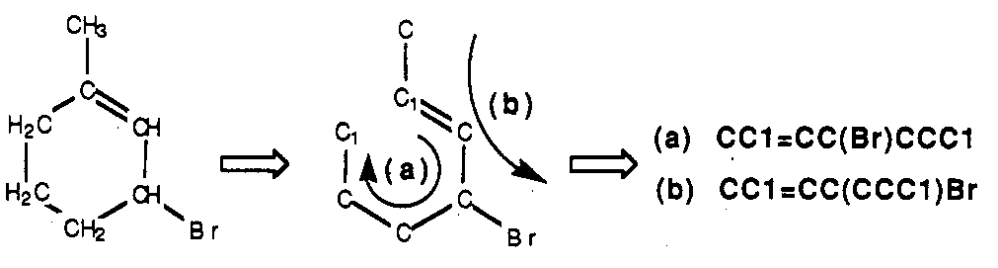
\includegraphics[scale=0.4]{imagenes/intro/sinonimos.png}
    \caption{Distintas cadenas SMILES válidas para el 1-methyl-3-bromo-ciclohexeno. \textbf{(a)} Considera el ciclo como la rama principal y el bromo como ramificación. \textbf{(b)} Hace el recorrido que marca la flecha, dejando parte del ciclo como una ramificación. Imagen extraída de \cite{weininger_smiles_1988}.}
    \label{fig:sinonimos_smiles}
\end{figure}

Esto tiene especial relevancia en el ámbito del Machine Learning (ML) o Aprendizaje Automático. Aunque se sale del alcance de este trabajo, uno de los grandes objetivos de la química computacional es la creación o diseño de nuevas moléculas. Se podrían crear modelos de ML, en particular de redes neuronales, capaces de generar moléculas ficticias válidas, para posteriormente ver sus propiedades, valorarlas energéticamente para ver cuán estables son y estudiar su viabilidad en distintas aplicaciones, entre otras cosas. SMILES dificulta esta tarea, y por ello, aparece en 2020, SELFIES (SELF-referencIng Embedded Strings), una nueva representación lineal 100\% robusta, muy usada actualmente para modelos generativos (ver \cite{SELFIES, krenn_self_referencing_2020} para más detalles de cómo soluciona los problemas de robustez y otras características de la representación). SELFIES es relativamente reciente por lo que aun no termina de instaurarse entre la comunidad investigadora, pese a esto, está continuamente ampliando sus funcionalidades, mejorando en simplicidad y facilidad de uso \cite{selfies_recent_2023}. Por último, InChI es creado en 2013 por la IUPAC (International Union of Pure and Applied Chemistry) como un proyecto para estandarizar el proceso de búsqueda de estructuras moleculares entre distintas bases de datos. Esto es porque InChI (International Chemical Identifier) genera una cadena canónica única para cada molécula, de manera que cada molécula tiene una sola representación, y dicha representación solamente hace referencia a esa molécula. La principal desventaja radica en su sintaxis y su estructura jerárquica, haciéndola complicada de leer y utilizar por los humanos. Por esto mismo, no es la mejor opción para usar en modelos generativos, pues tiene una serie de reglas y normas gramaticales y aritméticas que son complejas de aplicar al generar moléculas a través de modelos de ML \cite{heller_inchi_2015}. Por lo anteriormente comentado, por su uso tan extendido, por su facilidad de uso y legibilidad frente a las demás representaciones, me centraré en la notación SMILES durante el desarrollo de este trabajo. 

Desde la Universidad de Granada, la tutora de este TFG colabora con el grupo de investigación del ICIQ (Instituto Catalán de Investigación Química) liderado por la investigadora Mónica H. Pérez-Temprano\footnote{de aquí en adelante se hará referencia a esta colaboración como ``los expertos''}. Su foco de investigación gira en torno al entendimiento de transformaciones catalíticas en las que participan compuestos organometálicos, descubriendo y diseñando reacciones más eficientes basadas en catalizadores metálicos (para más detalle sobre el grupo de investigación y sus ámbitos de trabajo, ver su sitio web \cite{ICIQ}). En resumen, intentan desarrollar enfoques más sostenibles para la síntesis de moléculas orgánicas usando la química organometálica. Como tal, necesitan codificar correctamente una molécula de organometálica en pos de trabajar con ella adecuadamente y utilizar todas las herramientas, para, entre otras cosas, poder dibujarla y entenderla mejor.

Los químicos de este centro comentan que uno de los principales problemas que se detectan en este ámbito es la heterogeneidad en las distintas bases de datos para un mismo compuesto o molécula. Dicho esto, existen diversas bases de datos en química donde se recoge gran cantidad de información acerca de los compuestos. Entiéndase esto como una colección estructurada y organizada que contiene datos sobre compuestos químicos, sus propiedades y relaciones con otros compuestos. Se utilizan para almacenar y recuperar información sobre moléculas, sustancias, reacciones, propiedades fisicoquímicas, e incluso literatura científica relacionada. Mencionaré ahora las más importantes y las que serán objeto de interés:

\begin{itemize}
    \item \emph{SciFinder}, una herramienta de investigación muy potente que permite explorar las bases de datos de CAS (American Chemical Society) las cuales contienen literatura sobre Química y otras disciplinas afines como Física, Biomedicina, Geología, Ingeniería Química, etc. Incluye referencias bibliográficas y resúmenes de artículos, informes, y libros entre otras cosas. Permite realizar búsquedas por estructura, nombres de sustancias o identificadores, reacciones en la que participa dicha sustancia, artículos y publicaciones que nombren el compuesto en cuestión, e incluso proveedores de compra \cite{scifinder_website}. Para el uso de esta herramienta es necesario acceder mediante la red de una institución autorizada (en este caso trabajo mediante la VPN de la UGR) y seguir los pasos para registrarte\footnote{Pasos para el registro en SciFinder\url{https://bibliotecaugr.libguides.com/scifinder_scholar}}.

    \item \emph{Sigma-Aldrich}, una compañía de ciencia, química y biotecnología que se dedica a la producción y venta de productos químicos, reactivos, equipos y materiales de laboratorio. Ofrece herramientas, servicios, artículos y una gran variedad de productos químicos que se utilizan en investigación, biofarmacéutica, e industria entre otros ámbitos \cite{sigma_aldrich_web}. A través de su página web se enfocan al comercio electrónico pudiendo buscar y comprar productos, compuestos orgánicos e inorgánicos, agentes reactivos, isótopos para síntesis químicas, proteínas, enzimas, etc. De cada producto muestra información relevante como la ficha de datos de seguridad, detalles de las propiedades físicas y químicas así como algunas representaciones lineales del compuesto y la representación molecular en 2D.
    
    \item \emph{PubChem}, una base de datos abierta que sirve información a millones de usuarios en todo el mundo, desde investigadores y estudiantes hasta el público general. Recogen para cada compuesto, información sobre su estructura, representaciones 2D y 3D, identificadores, propiedades químicas y físicas, patentes, avisos de toxicidad, etc. \cite{pubchem_website} 
\end{itemize}
    
 Para ilustrar el problema de la heterogeneidad entre bases de datos, presento las Tablas \ref{tabla:tabla_peq_intro_sigmaAldrich} y \ref{tabla:tabla_peq_intro_sciFinder}. Ambas tablas comparan las mismas moléculas, mostrando el código SMILES y la representación visual que ofrecen las bases de datos Sigma-Aldrich y SciFinder respectivamente. Vemos diferencias claras en el tratamiento de los ciclos aromáticos, la especificación de las cargas de los átomos y la posición de algunas ramificaciones. Utilizo un subconjunto de 5 moléculas pertenecientes a la organometálica, seleccionadas desde un conjunto de datos de 30 moléculas considerados de interés por los químicos del ICIQ (disponible para su consulta en GitHub). En el Apéndice \ref{apend:pagina_tabla_intro_grande}, se puede consultar una tabla comparativa con el set de moléculas al completo. 





\begin{landscape}
    \begin{table}
  \begin{minipage}{.5\linewidth}
    \centering
    \begin{tabular}{m{0.3cm}m{4.8cm}>{\centering\arraybackslash}m{4cm}}
        \toprule
        \textbf{Id} & \textbf{Código SMILES} & \textbf{Representación 2D} \\
        \midrule
        1 &
        C[Au].c1ccc(cc1) P(c2ccccc2)c3ccccc3 & 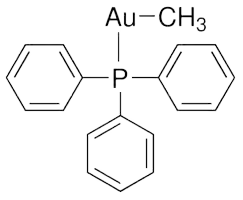
\includegraphics[width=2.7cm]{imagenes/sigmaAldrich/Methyl(triphenylphosphine)gold(I)} \\ [0.8cm]
        % \hline

        2 &
        Cl[Pd]Cl.C1CC=CCCC=C1 & 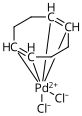
\includegraphics[width=2.8cm]{imagenes/sigmaAldrich/Dichloro(1,5-cyclooctadiene)palladium(II).png} \\ 
        % \hline
        
        3 &
        Cl[Au].CP(C)C & 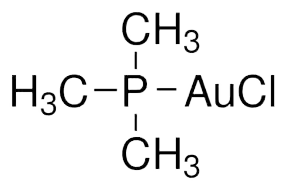
\includegraphics[width=2.8cm]{imagenes/sigmaAldrich/Chloro(trimethylphosphine)gold(I).png} \\ [0.8cm]
        % \hline

        4 &
        Cl[Au].CC(C)(C)P(c1ccccc1-c2ccccc2)C(C)(C)C & 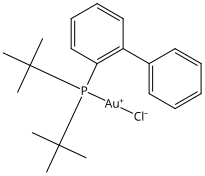
\includegraphics[width=2.8cm]{imagenes/sigmaAldrich/Chloro[(1,1-biphenyl-2-yl)di-tert-butylphosphine]gold(I).png} \\
        % \hline

        5 &
        [Fe]I.[C-]\#[O+].[C-]\#[O+].[CH]1[CH][CH][CH][CH]1 & 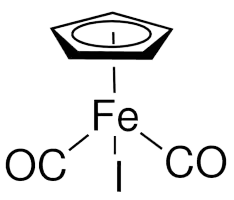
\includegraphics[width=2.7cm]{imagenes/sigmaAldrich/Dicarbonylcyclopentadienyliodoiron(II).png} \\
        \bottomrule
        \end{tabular}
    \caption{Códigos SMILES y sus representaciones visuales según Sigma-Aldrich}
    \label{tabla:tabla_peq_intro_sigmaAldrich}
  \end{minipage}%
  \begin{minipage}{.5\linewidth}
    \centering
    \begin{tabular}{m{0.1cm}m{4.8cm}>{\centering\arraybackslash}m{4cm}}
        \toprule
        & \textbf{Código SMILES} & \textbf{Representación 2D} \\
        \midrule
        &
        [Au+]([CH3-])[P] (C=1C=CC=CC1)(C=2C=C C=CC2)C=3C=CC=CC3 & 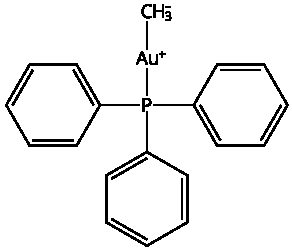
\includegraphics[width=2.2cm]{imagenes/sciFinder/pdf/Methyl(triphenylphosphine)gold(I).pdf} \\
        % \hline

        &
        [Cl-][Pd+2]123([Cl-]) [CH]=4CC[CH]3=[CH]2CC[CH]41 & 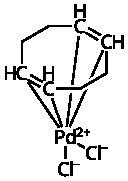
\includegraphics[width=2.2cm]{imagenes/sciFinder/pdf/Dichloro(1,5-cyclooctadiene)palladium(II).pdf} \\
        % \hline

        &
        [Cl-][Au+][P](C)(C)C & 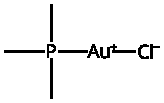
\includegraphics[width=2.2cm]{imagenes/sciFinder/pdf/Chloro(trimethylphosphine)gold(I).pdf} \\
        % \hline
        
        &
        [Cl-][Au+][P](C=1C=CC=C C1C=2C=CC=CC2) (C(C)(C)C)C(C)(C)C & 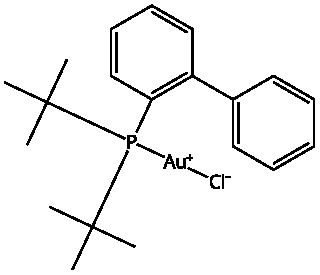
\includegraphics[width=2.2cm]{imagenes/sciFinder/pdf/Chloro[(1,1-biphenyl-2-yl)di-tert-butylphosphine]gold(I).pdf} \\
        % \hline
        
        &
        O\#C[Fe+2]1234([I-])(C\#O) [CH]=5[CH]4=[CH]3[CH-] 2[CH]51 & 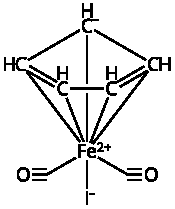
\includegraphics[width=2.2cm]{imagenes/sciFinder/pdf/Dicarbonylcyclopentadienyliodoiron(II).pdf} \\
        \bottomrule
        \end{tabular}
    \caption{Códigos SMILES y sus representaciones visuales según SciFinder}
    \label{tabla:tabla_peq_intro_sciFinder}
  \end{minipage}
\end{table}
\end{landscape}





\section{Objetivos}\label{objetivos}
El objetivo principal de este Trabajo Fin de Grado es mejorar las herramientas existentes para trabajar con chemoinformatics, adaptándolas a moléculas organometálicas y poder suplir los errores encontrados en las bases de datos disponibles. Para ello, se establecen los siguientes subobjetivos:
\begin{itemize}
    \item Analizar las distintas bases de datos químicas disponibles y evaluar similitudes y diferencias en el almacenado de moléculas organometálicas.
    \item Diseñar una metodología para representar de forma canónica una molécula organometálica. Esto es, una representación única y estandarizada para una molécula dada, independientemente de la forma en que se haya representado inicialmente.
    \item Mejorar la visualización de moléculas organometálicas.
\end{itemize} 

\section{Estructura de la memoria}
\begin{itemize}
    \item \textbf{Capítulo 1. Introducción}: se presenta el proyecto indicando la problemática a tratar, los motivos por los que se ha desarrollado y sus objetivos. 
    \item \textbf{Capítulo 2. Estado del arte y fundamentos teóricos}: breve revisión bibliográfica del tema del proyecto, estado de las soluciones actuales y conceptos teóricos necesarios para comprender el trabajo.
    \item \textbf{Capítulo 3. Gestión del proyecto y planificación}: descripción de la metodología de desarrollo seguida y planificación temporal. Se detalla también la gestión de recursos, el desglose del presupuesto y se realiza un análisis de riesgos del proyecto.
    \item \textbf{Capítulo 4. Diseño e implementación}: se describen las clases y métodos creados, dando una breve explicación de cada uno de ellos. Definición del sistema canónico alcanzado junto con sus reglas y los cambios en el sistema de representación 2D. 
    \item \textbf{Capítulo 5. Resultados y pruebas}: resultados generales tras la implementación y descripción de las pruebas llevadas a cabo.
    \item \textbf{Capítulo 6. Conclusiones y trabajos futuros}: exposición de las conclusiones del proyecto, y posibles ampliaciones para el futuro.
\end{itemize}



\chapter{Estado del arte y fundamentos teóricos}\label{estadoArte}

En este capítulo analizaré el estado actual del tema a tratar, junto con una pequeña revisión bibliográfica y algunos conceptos teóricos necesarios. También profundizaré un poco más en las representaciones lineales comentadas en el Capítulo \ref{introduccion}, así como los distintos paquetes software existentes y sus limitaciones. 

\section{Revisión bibliográfica} \label{revision_bib}
Para el estudio de los trabajos relacionados y búsqueda de bibliografía se han consultado fuentes como IEEE Xplore, ACS Publications, o Journal of Chemical Information and Computer Sciences, entre otras. En la Figura \ref{fig:revisionBibliografica} se exponen los resultados de un breve estudio bibliográfico sobre la literatura existente de los temas del proyecto. 

Todo comienza en 1988 con la publicación de David Weininger \cite{weininger_smiles_1988}, presentando SMILES como un nuevo formato de representación lineal, a partir de ahí y hasta día de hoy, fueron aumentando las publicaciones alrededor de SMILES. Sin embargo, vemos que apenas existe literatura para temas más específicos dentro de este área, como la canonización de las cadenas SMILES o la organometálica (ver Secciones \ref{teoria:representaciones_lineales} y \ref{teoria:ogm}). Además, si nos paramos a revisar las publicaciones existentes vemos que apenas ninguna coincide con los objetivos de este proyecto, y mucho menos hacen alguna propuesta de cómo darles solución. Los datos de las publicaciones se han recopilado a través de \textit{Scopus}\footnote{\url{https://www.elsevier.com/es-es/solutions/scopus}}\footnotecomma\footnote{\url{https://biblioteca.ugr.es/investigacion/herramientas-apoyo/evaluacion-publicaciones/scopus}} con las siguientes consultas, donde CHEM y COMP hacen referencia a chemistry y computer science respectivamente: 
\begin{itemize}
    \item {\footnotesize \textit{(SUBJAREA(CHEM) AND TITLE-ABS-KEY(smiles))}} 
    \item {\footnotesize \textit{((SUBJAREA(CHEM) OR SUBJAREA(COMP)) AND TITLE-ABS-KEY(smiles AND canonical))}}
    \item {\footnotesize \textit{(SUBJAREA(CHEM) AND TITLE-ABS-KEY(smiles AND organometallic))}}
\end{itemize}

\begin{figure}[h!]
        \centering
        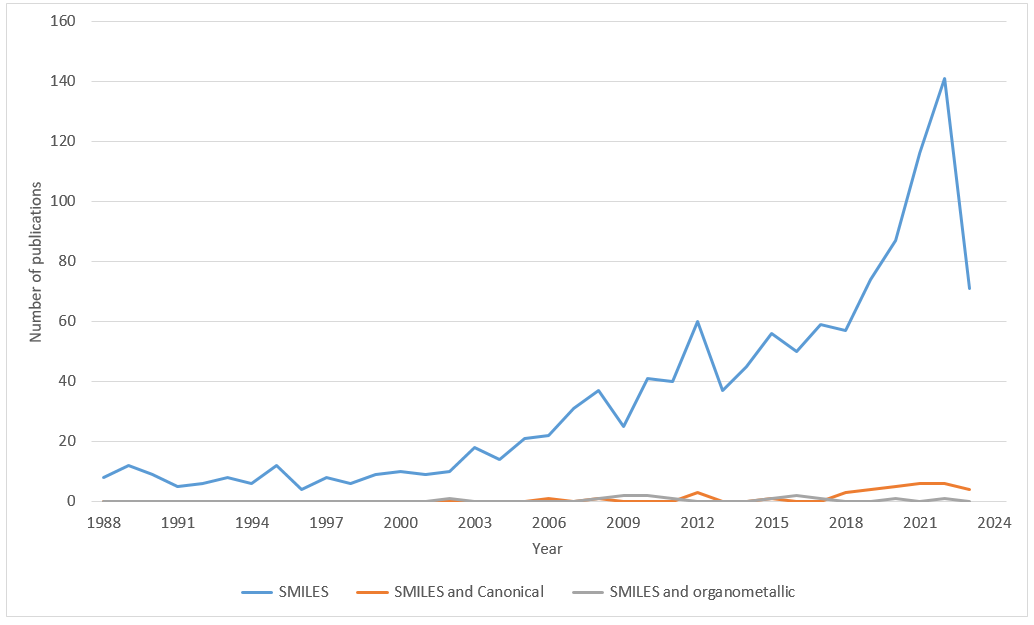
\includegraphics[scale=0.5]{imagenes/estado_arte/revisionBibliografica.png}
        \caption{Comparativa del número de artículos publicados por año según las palabras clave de la búsqueda. Imagen de elaboración propia. Datos extraídos de \emph{Scopus}.}
        \label{fig:revisionBibliografica}
    \end{figure}


\section{Fundamentos teóricos}

\subsection{Moléculas y sus representaciones}
representacion de moléculas (formula estructural conection tables, tipos de ficheros (.smi, .sdf, etc) representacion lineal y mas cosas),

\subsection{Representaciones lineales} \label{teoria:representaciones_lineales}
Hablar mas extendido de SMILES, SELFIES, e INCHI;

\subsection{Organometálica} \label{teoria:ogm}
Cualquier concepto de quimica que me haga falta para entender el trabajo, o que haya tenido que aprender yo durante el mismo.
hablar de la regla de los 18 electrones y compuestos de coordinacion vs organometalicos
(mirar mashup)
hablar de los electrones y bonds delocalized

Dentro de los compuestos organometálicos, los metalocenos son muy comunes y reconocibles. Estos se caracterizan por un catión metálico central, usualmente de un metal de transición, y dos ligandos orgánicos llamados ciclopentadienilos (Cp\footnote{en adelante se hará referencia como Cp})). Los ligandos Cp están formados por un anillo de cinco átomos de carbono unidos mediante enlaces covalentes. Estos ligandos Cp se unen al metal central mediante enlaces covalentes en donde cada átomo de carbono en el anillo Cp contribuye con un par de electrones pi para formar enlaces con el metal. Debido a la presencia de los enlaces pi, los metalocenos exhiben una gran estabilidad y reactividad química característica, lo que ha llevado a su amplio uso en catálisis y síntesis orgánica.
quizas pueda hablar de n5-coordination y todo esto (o es mucho detalle...)

En la siguiente Figura \ref{fig:metalocenos_ejemplos} podemos ver algunos ejemplos:
\begin{figure}[h!]
\centering
\begin{subfigure}{.5\textwidth}
  \centering
  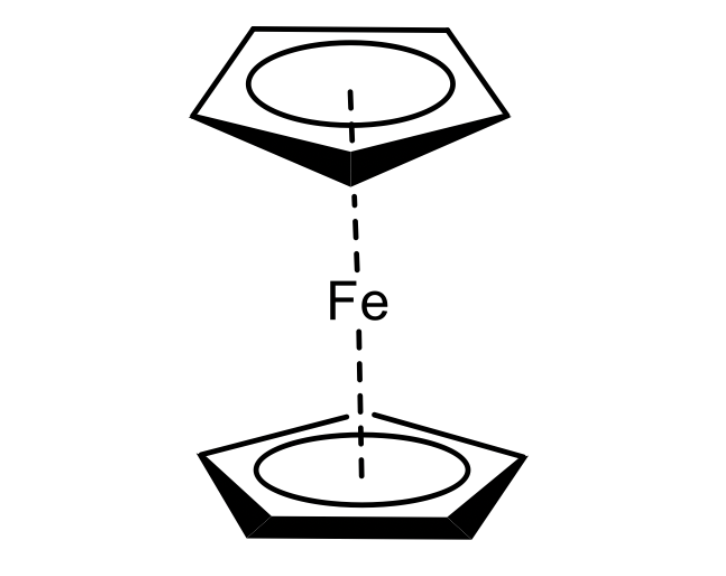
\includegraphics[width=.7\linewidth]{imagenes/estado_arte/teoria/ferroceno.png}
  \caption{}
  \label{fig:sub1}
\end{subfigure}%
\begin{subfigure}{.5\textwidth}
  \centering
  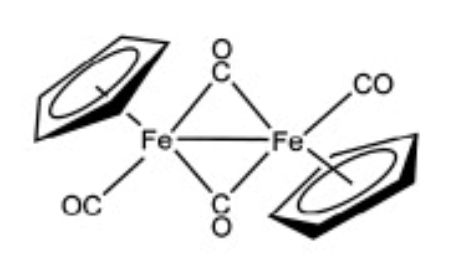
\includegraphics[width=.9\linewidth]{imagenes/estado_arte/teoria/derivativo_ferreoceno.png}
  \caption{}
  \label{fig:sub2}
\end{subfigure}
\caption{Representaciones 2D. \textbf{(a)} compuesto de ferroceno, que consta de un átomo de hierro central enlazado con 2 Cp; \textbf{(b)} derivativo del Dicarbonylcyclopentadienyliron. Imágenes extraídas de \cite{libreTextMetalocenos, artero_hydrogen_2008} respectivamente.}
\label{fig:metalocenos_ejemplos}
\end{figure}

\section{Herramientas o toolkits} \label{toolkits}

Existe una gran variedad de herramientas a la hora de trabajar dentro de la química computacional, tanto open-source como aplicaciones propietarias para las que son necesarias pagar una licencia de uso. La química computacional según comenté en el Capítulo \ref{introduccion}, se aplica en muchos ámbitos de la ciencia. Como tal, hay herramientas con propósitos muy distintos \cite{toolkits_recap}: 
\begin{itemize}
    \item Extensiones de navegador que mejoran el acceso a la información de las bases de datos \cite{safari_extensions}.
    \item Cálculos de propiedades fisicoquímicas (casi cualquier herramienta lo permite).
    \item Cribado virtual de moléculas como \textit{ChemAxon}, \textit{MOE}, \textit{LigandScout} o \textit{Forge}.
    \item Modelado y bocetado de moléculas como \textit{Marvin}, \textit{ChemDraw} o \textit{ChemDoodle}.
    \item Hojas de cálculo con análisis de datos químicos como \textit{Vortex}.
    \item Toolkits de propósito general con diversas funcionalidades básicas como \textit{OpenBabel} o \textit{RDKit}.
\end{itemize}
Las herramientas más complejas o relacionadas de alguna manera con la medicina suelen ser de pago. Para los objetivos de este proyecto se han tenido en cuenta los toolkits de propósito general mencionados anteriormente que son capaces de trabajar con SMILES.

\subsection{OpenBabel y RDKit}

Openbabel y RDKit son bastante parecidos en cuanto a sus funcionalidades, ambos permiten la manipulación de estructuras químicas, cálculos de propiedades moleculares, análisis de similitudes entre moléculas, generación de representaciones 2D y conversión entre distintos tipos de ficheros. Para elegir entre una de estas 2 herramientas, se han hecho pruebas iniciales en un notebook de Google Colab \cite{google_colab} (disponible el en GitHub de este proyecto).


RDKit por su parte, consigue representaciones 2D parecidas o mejores que las de OpenBabel para moléculas pequeñas y cuenta con mayores opciones de personalización del dibujo resultado \cite{rdkit_cookbook} haciéndolo más visual. Además, es más preciso a la hora de representar la estereoquímica, algo en lo que OpenBabel es bastante pobre. Vemos en la Figura \ref{fig:ejemplo_rdkit_vs_babel} un ejemplo con ambos paquetes software. Sin embargo, si se le exige un poco más a RDKit pidiéndole moléculas complejas no funciona del todo bien. Concretamente, cuando introducimos moléculas de organometálica no las lee correctamente aun siendo químicamente válidas. RDKit lleva a cabo un proceso de 'saneamiento' (\textit{sanitization}) \cite{rdkit_docbook} por el que, además de calcular algunas propiedades útiles (pertenencia de los átomos a anillos o hibridaciones), comprueba que la molécula de entrada es 'razonable'. Para RDKit, serán razonables las moléculas que cumplan la regla del octeto \cite{lewis2} y puedan representarse mediante las estructuras de Lewis de manera completa \cite{lewis_2013, lewis2}. Como hemos visto anteriormente, los compuestos de coordinación se rigen por otro tipo de sistema de valencia, y RDKit no es capaz de trabajar con esta clase de moléculas. De hecho, del set de moléculas del que dispongo para el proyecto, no es capaz de leer ningún código SMILES de los que fueron extraídos de SciFinder. Los SMILES de SigmaAldrich si los puede usar, pero más adelante en esta misma sección se explicará porqué estos no nos sirven.

\begin{figure}[h!]
\centering
\begin{subfigure}{.5\textwidth}
  \centering
  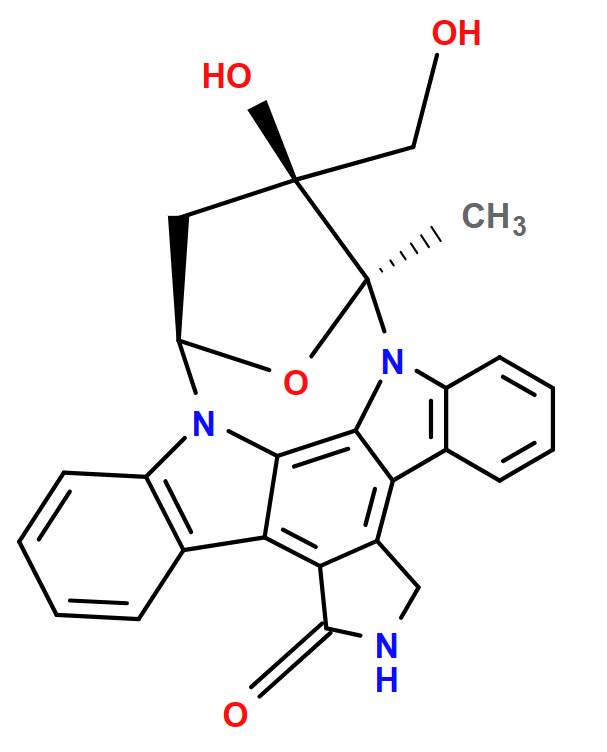
\includegraphics[width=.7\linewidth]{imagenes/estado_arte/Lestaurtinib_openbabel.png}
  \caption{OpenBabel}
  \label{fig:sub1}
\end{subfigure}%
\begin{subfigure}{.5\textwidth}
  \centering
  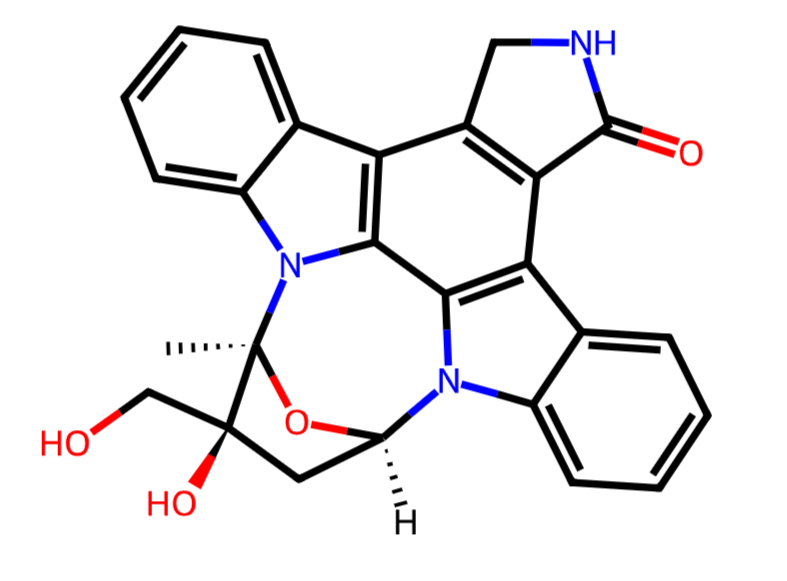
\includegraphics[width=.9\linewidth]{imagenes/estado_arte/Lestaurtinib_rdkit.png}
  \caption{RDKit}
  \label{fig:sub2}
\end{subfigure}
\caption{Representaciones 2D para el \emph{Lestaurtinib}, medicamento en estudio para el tratamiento de las leucemias agudas y algunos otros tipos de cáncer. \textbf{(a)} ha sido generado con OpenBabel; y \textbf{(b)} ha sido generado con RDKit.}
\label{fig:ejemplo_rdkit_vs_babel}
\end{figure}



OpenBabel por otro lado, ofrece más libertad en este sentido siendo capaz de leer todos los SMILES del set del que partimos. Pero en general, algo que hacen mal ambos paquetes es representar moléculas en 2D. Para moléculas convencionales, moléculas orgánicas o inorgánicas sencillas funciona bien, pero las organometálicas les supone un reto, y dada la escasa literatura en el tema (ver Sección \ref{revision_bib}), no dispongo de muchas referencias de las que partir.


En cuanto a los datos de partida contamos con 2 versiones de SMILES, los provenientes de SigmaAldrich y los de SciFinder. Siguiendo la comparación de la Sección \ref{motivacion} ambos SMILES son notablemente distintos, de hecho no se podrían considerar ni siquiera sinónimos ya que al de SigmaAldrich le faltan enlaces, y no llegan a codificar la misma molécula. Tanto es así que las cadenas SMILES que contienen desconexiones (representadas por el punto '.') no nos son para nada útiles. Al fragmentar la molécula estamos perdiendo los enlaces entre los átomos, una información muy valiosa para la mayoría de operaciones. Como se dijo antes (\textbf{me falta mencionar esto en los fundamentos teoricos}), una molécula se suele almacenar principalmente identificando sus átomos y los enlaces entre sus átomos. Podríamos decir que se está perdiendo casi la mitad de la información acerca de la molécula, y dado que uno mismo no puede inventarse los enlaces, no es un buen SMILES para nuestros objetivos, ni para la canonización ni para el dibujado. En la Figura \ref{fig:dotted_smiles_vs_complete} vemos la diferencia entre la representación de un SMILES inconexo frente a uno con buena conectividad.


\begin{figure}[h!]
\centering
\begin{subfigure}{.5\textwidth}
  \centering
  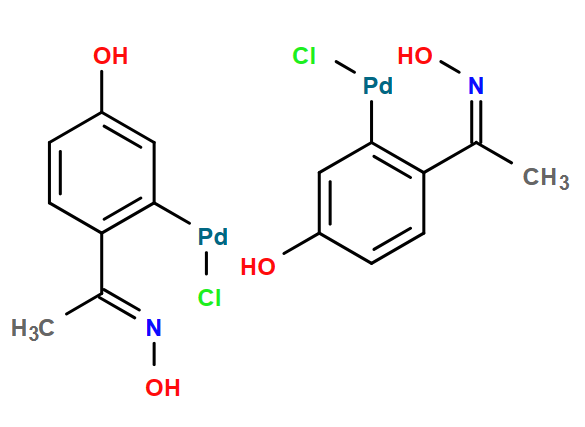
\includegraphics[width=.9\linewidth, frame]{imagenes/estado_arte/dotted_SA.png}
  \caption{}
  \label{fig:sub1}
\end{subfigure}%
\begin{subfigure}{.5\textwidth}
  \centering
  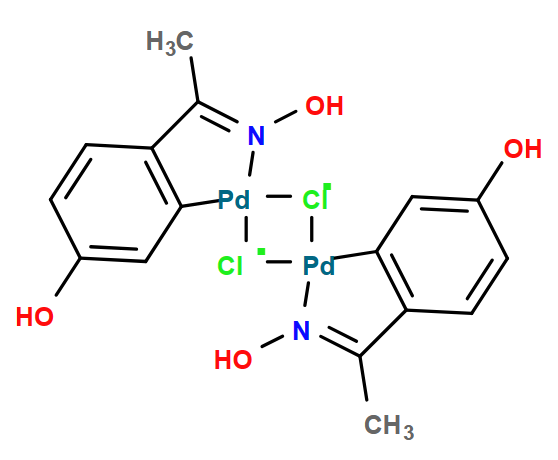
\includegraphics[width=.8\linewidth, frame]{imagenes/estado_arte/not_dotted_SF.png}
  \caption{}
  \label{fig:sub2}
\end{subfigure}
\caption{Representaciones 2D generadas con OpenBabel para el \emph{'Nájera Catalyst II'}. \textbf{(a)} SMILES con desconexiones extraído de SigmaAldrich; y \textbf{(b)} SMILES conectado extraído de SciFinder.}
\label{fig:dotted_smiles_vs_complete}
\end{figure}


\subsection{Herramientas de bocetado}
Existen herramientas tipo ChemDraw \cite{chemdraw_page}, que son las que los químicos e investigadores utilizan para dibujar manualmente las moléculas que luego añaden a sus publicaciones. Son este tipo de dibujos también los que probablemente podemos ver en algunas bases de datos como SigmaAldrich. En la Figura \ref{fig:chemdraw} se muestra su interfaz y algunas moléculas bocetadas.

\begin{figure}[h!]
    \centering
    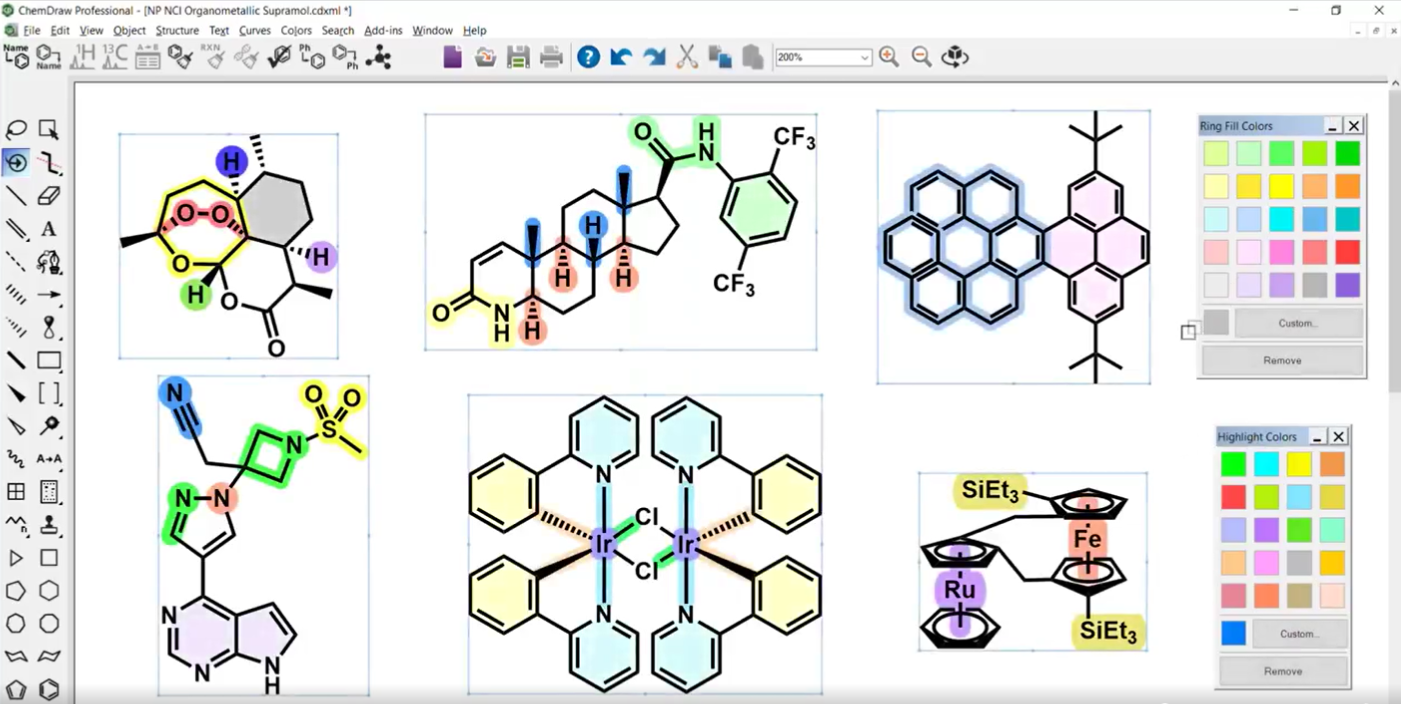
\includegraphics[scale=0.34]{imagenes/estado_arte/chemdraw.png}
    \caption{Interfaz de ChemDraw con algunas moléculas de prueba bocetadas. Imagen extraída de su página oficial \cite{chemdraw_page}}
    \label{fig:chemdraw}
\end{figure}

\subsection{Nomenclatura canónica}
Como ya se ha visto, InChI proporciona una representación canónica para las moléculas, lo que permite una vinculación directa y unívoca entre las bases de datos. SMILES por otro lado complica este proceso. SMILES fue desarrollado en su momento como un software propietario por Daylight Chemical Information Systems (Daylight) \cite{daylight}, y desde su introducción a finales de los 80 se ha extendido como una norma de facto para representar estructuras moleculares. En base a esto y con el tiempo, se han escrito en varios lenguajes de programación muchos paquetes de software independientes que trabajan con SMILES\cite{opensmiles}.

Bien es cierto que hay cada vez más propuestas de cómo alcanzar una nomenclatura única \cite{weininger_smiles_1989, inchi1, nextmove_software_facto_nodate, baoilleach_we_nodate, universal_smiles} y ya existen algunas reglas definidas para la química orgánica a la hora de establecer prioridades entre los átomos y ordenar la molécula. Véase por ejemplo las \emph{'Reglas de Cahn-Ingold-Prelog'} aplicadas a enantiómeros \cite{cahn_specification_1966, prelog_basic_1982, NOMENCLATURA_R_S} para definir órdenes levógiros o dextrógiros (no abordaremos esto, excede el alcance del proyecto). Pero trasladar estas reglas a compuestos organometálicos es complicado, además de haber multitud de excepciones, en la mayoría de casos un mismo fragmento está enlazado por varios sitios al metal y hay que definir el átomo inicial por el que empezar a recorrer la molécula. Al final, cada paquete software implementa esta decisión de una manera diferente usando un algoritmo propio, obteniendo así lo que cada uno de ellos nombra como 'canonical SMILES', pero siguen siendo distintos entre ellos, por lo que no es canónico.

\subsection{Conclusiones}
Dicho todo lo anterior, durante las pruebas realizadas se ha podido comprobar y extraer las siguientes conclusiones:

\begin{itemize}
    \item Al representar la misma molécula con herramientas distintas, lo normal es que generen dibujos diferentes, en donde uno será mejor o más correcto que el otro.
    \item Para una misma molécula es probable que cada base de datos muestre una cadena SMILES diferente y una representación 2D distinta. De hecho, la imagen puede ni siquiera concordar con el SMILES que ofrecen, apareciendo en multitud de casos por ejemplo, un SMILES desconectado y una imagen con la molécula al completo (lo más seguro es que estén hechos a mano)
    \item Vistos los resultados de los SMILES de SigmaAldrich, para el resto del proyecto se asumirá que se trabaja con los SMILES de SciFinder, ya que dotan de mejor conectividad. 
    \item Debido a lo anterior, y como RDKit no soporta los datos de entrada, se utilizará la librería de OpenBabel para el proyecto.
    \item Hay diversos tipos de compuestos que no se describen bien mediante la representación de su grafo molecular, como los compuestos de coordinación. Su sistema de enlaces no se ajusta a la teoría de los enlaces de valencia, por lo que es complejo describir sus enlaces mediante relaciones 1 a 1 entre los átomos \cite{david_molecular_2020}.
    \item Moléculas complejas con multitud de ciclos o muchos enlaces al mismo átomo (generalmente un metal), Openbabel genera unas representaciones 2D muy agrupadas, con los enlaces superpuestos y partes del dibujo unas encima de las otras, dificultando su entendimiento.
    \item Hasta el mommento, no hay ningún sistema de canonizado que trabaje de manera eficiente con moléculas organometálicas.
    
\end{itemize}


Teniendo esto en cuenta y lo mencionado en la Sección \ref{motivacion}, en las siguientes secciones se dará pie a la implementación de una propuesta de nomenclatura canónica para moléculas organometálicas y la mejora del dibujado de las mismas con OpenBabel.







\chapter{Gestión y Planificación del proyecto}


\section{Metodología}

En el pasado, el desarrollo de software seguía un enfoque \textit{ad hoc} (software a medida) y poco estructurado, lo que llevaba a problemas como retrasos, presupuestos desbordados, productos finales que no cumplían con las expectativas o proyectos inmanejables y difíciles de mantener. Era frecuente por tanto proyectos fallidos o de mala calidad. Como resultado, surgió la necesidad de establecer un marco de trabajo más formal y disciplinado para el desarrollo de software. Las metodologías de desarrollo proporcionan pues, un marco de trabajo y un conjunto de métodos que guían a los equipos de desarrollo a lo largo del ciclo de vida del proyecto. Es por tanto, a día de hoy, fundamental elegir una metodología que se adapte bien al proyecto.
Por lo general, las metodologías de desarrollo se clasifican en dos grandes grupos, tradicionales y ágiles. Se resume en la Tabla \ref{tabla:resumen_trad_agil}, las diferencias entre ambas metodologías. 


\begin{table}[h!]
    \centering
    \begin{tabular}[t]{lll}
        \toprule
         & \textbf{Tradicionales} & \textbf{Ágiles} \\
        \midrule
        \textbf{Enfoque} & Secuencial & Iterativo e incremental   \\
        \midrule
        \textbf{Planificación} & Detallada y exhaustiva & Adaptativa y flexible   \\
        \midrule
        \textbf{Gestión cambios} & Difícil de manejar & Fomenta la adaptabilidad   \\
        \midrule
        \textbf{Requisitos} & Definidos desde el inicio & Evolucionan con el tiempo     \\
        \midrule
       \textbf{Entrega software} & Al final del proyecto & Continua, en incrementos      \\
        \midrule
        \textbf{Colaboración} & Menos énfasis & Fomenta la colaboración      \\
        \midrule
        \textbf{Equipos} & Mejor en equipos grandes & Mejor en equipos pequeños      \\
        \midrule
        \textbf{Adaptabilidad} & Menor flexibilidad & Mayor flexibilidad      \\
        \midrule
        \textbf{Retroalimentación} & Al final del proyecto & Constante y temprana      \\
        \bottomrule
    \end{tabular}
    \caption{Tabla comparativa de las principales características entre las metodologías tradicionales y ágiles}
    \label{tabla:resumen_trad_agil}
\end{table}


Para este proyecto hay varias razones por las cuales elegir una metodología ágil:
\begin{itemize}
    \item Se trata de un proyecto de investigación, donde se intentarán desarrollar varios algoritmos para la resolución de un problema. Por lo que, a priori no se conoce la calidad de los resultados que se obtendrán. Se deberán realizan experimentos iniciales para detectar los problemas, desarrollar una posible solución y volver a realizar experimentos para evaluar los resultados hasta alcanzar unos que cumplan con los objetivos o sean lo suficientemente satisfactorios.
    \item Se hará uso de herramientas en las que no se posee experiencia previa, lo que podrá originar retrasos en la planificación o modificaciones frecuentes.
    \item Las metodologías ágiles se ajustan mejor en equipos pequeños como indico en la Tabla \ref{tabla:resumen_trad_agil}. En este caso el equipo de trabajo solo tiene una persona.
    \item La figura del tutor y la experta en química del ICIQ serán importantes para dar feedback continuo durante el proyecto y opinar sobre la calidad de los resultados.
\end{itemize}

Por las anteriores razones, una metodolgía clásica no se adaptaría bien al proyecto, prefiriendo una ágil. Permite una mayor flexibilidad con las tareas, y un desarrollo incremental en base a los resultados intermedios que se vayan obteniendo.


Dentro de las ágiles existen varias metodologías como Scrum, eXtreme Programming, Lean Development, Kanban, Crystal, DSDM, etc. Las más comunes hoy día son Scrum y XP, al ser las que mejores resultados obtienen en proyectos de desarrollo software \cite{15_agile_report, fuior_key_2019, despa_comparative_2014, mishra_organizational_2021}. Hay que tener en cuenta que la mayoría de metodologías imponen una serie de prácticas y principios para guiar al equipo de desarrollo durante el proyecto. A algunos autores como Mike Cohn (fundador de la Scrum Alliance) les gusta tratar las metodologías como marcos de trabajo y no como una serie de métodos y reglas estrictas que haya que seguir al pie de la letra \cite{cohn_differences_2007}. 

El perfil del proyecto no terminaba de encajar con ninguna metodología al completo, por lo que se ha aplicado un híbrido entre Scrum y XP, mezclando aspectos y técnicas de ambas según se ajustaban al proyecto. Scrum maneja la parte administrativa del proyecto, definiendo cómo se especifica el trabajo y el proceso de entrega de características, mientras se aplican algunas prácticas propias de XP para la parte de codificación\cite{salazar_scrum_2018, linkedin_hybrid_xp_scrum}

\subsection{Scrum}

\begin{figure}[H]
    \centering{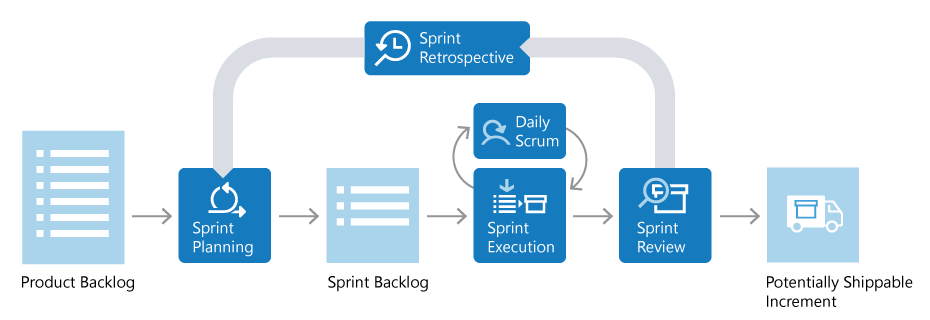
\includegraphics[scale=0.64]{imagenes/planificacion/agile-scrum-lifecycle-diagram.png}}
    \caption{Ciclo de vida iterativo de Scrum.}
    \label{fig:scrum_ciclo_vida}
\end{figure}
El ciclo de vida de Scrum (Figura \ref{fig:scrum_ciclo_vida}, extraída de Microsoft learn\footnote{\url{https://www.scrum.org/}}) se basa en un enfoque iterativo e incremental que permite a los equipos adaptarse a los cambios y entregar productos de alta calidad en un tiempo reducido. Los principios de transparencia, inspección y adaptación son fundamentales para alcanzar los valores centrales de Scrum, la calidad, flexibilidad, mejora continua, compromiso, coraje, ritmo y responsabilidad. 
Una de las características principales de Scrum es su enfoque en ciclos de desarrollo cortos llamados \emph{sprints}. Estos sprints suelen tener una duración de una a cuatro semanas, durante los cuales se planifican, desarrollan, prueban y entregan incrementos de software funcionales. Cada sprint comienza con una reunión de planificación en la que el equipo selecciona un conjunto de tareas para ser completados durante el sprint. Podemos definir Scrum según los elementos que lo componen:

\begin{itemize}
    \item \textbf{Artefactos}
    \begin{itemize}
        \item \textbf{Product Backlog (Pila del producto)}: es una lista ordenada y priorizada de todas las funcionalidades, características y mejoras que podrían ser necesarias para el producto. Es responsabilidad del Product Owner y se actualiza constantemente a medida que se obtiene nueva información o se generan cambios en los requisitos.
        \item \textbf{Sprint Backlog (Pila del sprint)}: es un conjunto de elementos seleccionado del Product Backlog para el sprint. Se descomponen en tareas de desarrollo más pequeñas junto con estimaciones de tiempo, expresando los requisitos en lenguaje técnico.
    \end{itemize}
        

    \item \textbf{Reuniones}
    \begin{itemize}
        \item \textbf{Sprint Planning}: marca el inicio de cada sprint y se realiza con el propósito de identificar el objetivo principal del sprint y las tareas concretas que se van a desarrollar en él. Como resultado, se genera el Sprint Backlog.
        \item \textbf{Daily Meetings}: reunión diaria de unos 15 minutos donde participan los miembros del Equipo de Desarrollo y el Scrum Master. Es una manera de estar al tanto del trabajo realizado y cuáles son los siguientes pasos. Es una oportunidad de identificar rápidamente obstáculos o problemas.
        \item \textbf{Sprint Review}: al final del sprint se pone en común todo el trabajo realizado durante el Sprint. Sirve para recoger información o feedback sobre el estado del proyecto.
        \item \textbf{Sprint Retrospective}: el equipo dedica tiempo a reflexionar sobre los aspectos positivos y las áreas que requieren mejoras. Como resultado de la retrospectiva, se generan acciones específicas para implementar en el siguiente sprint.
    \end{itemize}

    \item \textbf{Roles}: representan responsabilidades dentro del proyecto.
    \begin{itemize}
        \item \textbf{Stakeholders}: son todos aquellos interesados en el proyecto, tanto personas como organizaciones (gente de marketing, comerciales, usuarios, etc).
        \item \textbf{Product Owner (PO, propietario)}: debe conocer perfectamente el entorno de negocio del cliente, las necesidades y el objetivo que se persigue con el sistema que se está construyendo. Debe conocer también como funciona Scrum para desempeñar bien su rol. Su responsabilidad principal es la de crear, administrar, y priorizar el P.Backlog, así como validar o rechazar el incremento resultado de cada iteración.
        \item \textbf{Scrum Master (director del proyecto)}: garantiza el correcto funcionamiento de los procesos y metodologías que se empleen en el equipo. Gestiona el proceso e intenta mejorar la productividad del equipo. Promueve los valores y prácticas de Scrum, elimina impedimentos, facilita la colaboración entre los roles, actúa como escudo ante cosas externas. Se asegura de que el PO sepa cómo ordenar la pila de producto para maximizar el valor generado en cada sprint.
        \item \textbf{Equipo de desarrollo}: es el que se encarga de desarrollar el producto y hacer los entregables en incrementos. Los miembros del equipo necesitan ser auto-organizados, multidisciplinares, multifuncionales, con un alto compromiso y sin jerarquías internas. Son los verdaderos responsables de que el producto salga adelante y se completen los incrementos. Se encargan de estimar el tamaño de los ítems del backlog. Es importante que el equipo de desarrollo comprenda bien la visión que tiene el PO acerca del producto. Suelen estar formados de entre 5 a 9 personas.
    \end{itemize}
\end{itemize}

\subsection{XP}
La programación extrema (XP) es una metodología ágil que se centra en la velocidad y la simplicidad con ciclos de desarrollo muy cortos. En XP se promueven una serie de valores: comunicación, simplicidad, retroalimentación, coraje y respeto \cite{salazar_scrum_2018}. Diseñada para entornos dinámicos con requisitos cambiantes y orientado fuertemente hacia la codificación, reduciendo considerablemente la documentación. En XP, las tareas que se terminan son susceptibles de ser modificadas durante el transcurso del proyecto, incluso después de que funcionen correctamente, por lo que son importantes las siguientes prácticas.

\begin{itemize}
    \item \textbf{Prácticas}: XP propone una serie de prácticas a nivel técnico que se deberían adoptar para el desarrollo del proyecto \cite{extremeXP_Page}. Las más importantes a mi parecer son:
    \begin{itemize}
        \item \textbf{Programación a pares}: los programadores trabajan en parejas, mientras uno escribe el código, el otro proporciona comentarios y realiza revisiones en tiempo real. Esto promueve el intercambio de conocimientos, la revisión de código constante y la minimización de errores.
        \item \textbf{Propiedad colectiva del código}: la propiedad colectiva anima a todos a aportar nuevas ideas sobre todos los segmentos del proyecto. Cualquier desarrollador puede cambiar cualquier línea de código para añadir funcionalidad, corregir errores, mejorar diseños o refactorizar.
        \item \textbf{Estándares de codificación}: el código ajustarse a las normas de codificación acordadas. Estas hacen que el código sea consistente y fácil de leer y refactorizar para todo el equipo. Un código con el mismo aspecto o que sigue unas normas fomenta la propiedad colectiva.
        \item \textbf{Marcha sostenible}: encontrar un ritmo de trabajo para el equipo de desarrollo donde todos los miembros se sientan cómodos. Las horas extra acaban con el espíritu y la motivación del equipo. A veces, menos es más.
        \item \textbf{Integración continua}: los equipos de XP no esperan a que se completen las iteraciones, sino que se integran constantemente. Se cuenta con un repositorio de código donde los desarrolladores envían el código cada poco tiempo.
        \item \textbf{Refactorización}: reescribir ciertas partes del código para aumentar su legibilidad y mantenibilidad pero sin modificar su comportamiento. Las pruebas han de garantizar que en la refactorización no se ha introducido ningún fallo. Evita la complejidad innecesaria.
        \item \textbf{Desarrollo orientado a pruebas}: las pruebas son frecuentemente repetidas y automatizadas cada vez que se haga un cambio, por pequeño que sea, antes de desplegar la nueva versión. Se suelen escribir antes que el propio código.
    \end{itemize}
    
    \item \textbf{Roles}
    \begin{itemize}
        \item \textbf{Programador}: encargados de escribir y probar el código.
        \item \textbf{Cliente}: representa los intereses del usuario y es responsable de proporcionar las necesidades, requisitos del software y establecer prioridades. 
        \item \textbf{Entrenador (Coach)}: es el líder del equipo, actúa como facilitador y promotor de las prácticas y valores de XP, y ayuda al equipo a mejorar y adaptarse.
        \item \textbf{Consultor}: miembro externo al equipo de desarrollo con conocimiento específico en un tema necesario.
        \item \textbf{Rastreador (Tracker)}: se encarga de gestionar la planificación y llevar un seguimiento del proyecto detectando los problemas en él.
    \end{itemize}
\end{itemize}

\subsection{Aplicación de Scrum/XP al proyecto} \label{aplicacion_metod}

Algunas de las características y prácticas mencionadas de cada una de las metodologías no son aplicables al proyecto dada su naturaleza e integrantes, como por ejemplo, la programación por parejas propia de XP. Se describe ahora, el enfoque que se le ha dado del híbrido Scrum/XP al proyecto.

Se lleva a cabo una planificación por \emph{Sprints} de entre 2 a 4 semanas, dependiendo de las tareas a realizar. Entre medias y al final de cada sprint, se agendará una \emph{reunión con la tutora} en la que se hará retrospectiva del mismo, para comprobar el estado y avance del proyecto. Se revisará qué se ha hecho durante el sprint y cómo se ha hecho, repasando las novedades desde la última iteración y puntos a mejorar o pulir, priorizando las siguientes tareas a realizar en base a los resultados. Igualmente, se mantendrá el contacto con el tutor de manera constante vía correo electrónico.


Mediante la \emph{integración continua}, los cambios se envían con frecuencia a un repositorio compartido con un sistema de control de versiones. Cada vez que se realiza un cambio o se desarrolla una nueva funcionalidad, se ejecutan \emph{pruebas} en el dataset completo de moléculas, comprobando rápidamente si los resultados son los esperados (parcial o totalmente), y detectar cualquier error antes de que se convierta en un problema más grave. Se sigue por tanto un \emph{desarrollo incremental}, añadiendo pequeñas funcionalidades o porciones de código funcional, centrándome en un aspecto específico en cada commit subido a github.

Se asignarán los roles propios de Scrum. El papel de \emph{Equipo de desarrollo} recae sobre el estudiante, y al ser únicamente una persona, también actuará como \emph{Scrum Master} siendo responsable de la correcta aplicación de la metodología y prácticas al proyecto. La tutora actuará como \emph{Product Owner}, conoce las necesidades del proyecto y el dominio del problema, hace de intermediaria con el cliente y ayuda al equipo de desarrollo a priorizar las tareas. Como posibles clientes o personas interesadas (\emph{stakeholders}) podemos incluir al grupo de investigación del ICIQ, con el que se mantiene el contacto frecuentemente a través del Product Owner.

Al ser OpenBabel una librería existente es importante mantener unos \emph{estándares de codificación} y un estilo consistente. Teniendo eso en mente, y usando el \emph{Refactoring}, se realizan cambios manteniendo el código limpio y legible. Se han usado las guías propias de OpenBabel y la documentación oficial orientada a desarrolladores para añadir nuevas funcionalidades\footnote{\url{https://openbabel.org/docs/current/OpenBabel.pdf}}\footnotecomma \footnote{\url{https://acortar.link/Openbabel_Adding_Plugins}}. Además, se busca ante todo la simplicidad a la hora de programar, evitando añadir funcionalidades extremadamente complejas o innecesarias y la adopción de soluciones sencillas.

\section{Planificación}
Inicialmente se elaboró una planificación estimada general, dividida en bloques grandes de trabajo, para establecer marcos de tiempo y controlar el ritmo del proyecto. Se puede ver en la Figura \ref{fig:gantt_incial_estimado}
\begin{figure}[h!]
    \centering
    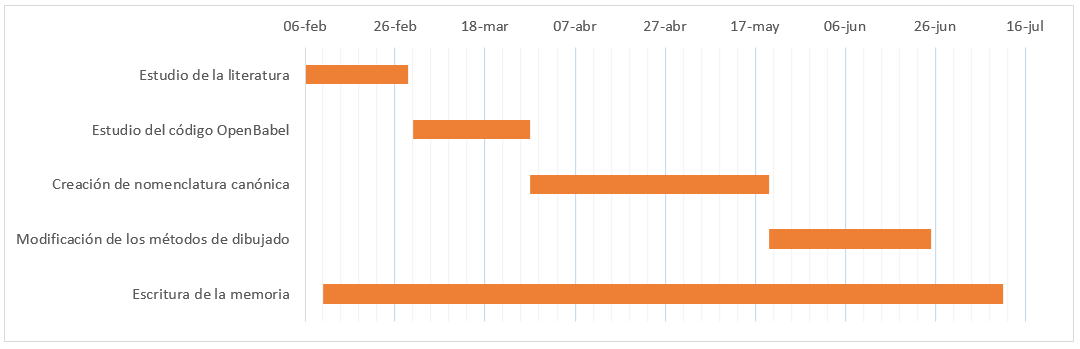
\includegraphics[scale=0.43]{imagenes/planificacion/planificacion_estimada.png}
    \caption{Diagrama de Gantt sobre la planificación inicial estimada}
    \label{fig:gantt_incial_estimado}
\end{figure}

Conforme se iba profundizando en el dominio del problema y entendiendo más sobre la problemática, se fueron subdividiendo y priorizando las tareas. A continuación, se desglosan las tareas definidas para el proyecto, separados en sprints: 

\begin{itemize}
    \item \textbf{Bloque 1}: Investigación y aprendizaje previo. Estudio del estado del arte.
    \begin{itemize}
        \item Lectura artículos y publicaciones sobre Chemoinformatics
        \item Repaso de química general y estudio de química organometálica
        \item Experimentación y pruebas iniciales con distintas herramientas
    \end{itemize}

    \item \textbf{Bloque 2}: Estudio del paquete OpenBabel
    \begin{itemize}
        \item Lectura detallada del código OpenBabel
        \item Experimentación moléculas usando el dibujado de OpenBabel
    \end{itemize}

    \item \textbf{Bloque 3}: Proceso de mejora del sistema de dibujado
    \begin{itemize}
        \item Detección de estructuras de ciclopentadienilo (Cp)
        \item Modificación dibujado moléculas con Cp individuales
        \item Detección de múltiples Cp en la misma molécula usando bloques
    \end{itemize}

    \item \textbf{Bloque 4}: Creación de nomenclatura canónica
    \begin{itemize}
        \item Detección de bloques en el SMILES y creación del árbol genérico
        \item Desarrollo del algoritmo canónico para moléculas con 1 metal
        \item Algoritmo canónico para moléculas con 2 o más metales
    \end{itemize}

    \item \textbf{Bloque 5}: Documentación del proyecto
    \begin{itemize}
        \item Redacción de la memoria
    \end{itemize}
\end{itemize}


\begin{landscape}

En el siguiente Diagrama de Gantt (Figura \ref{fig:gantt_real}) se presenta la planificación real del proyecto:

    \begin{figure}[h!]
        \centering
        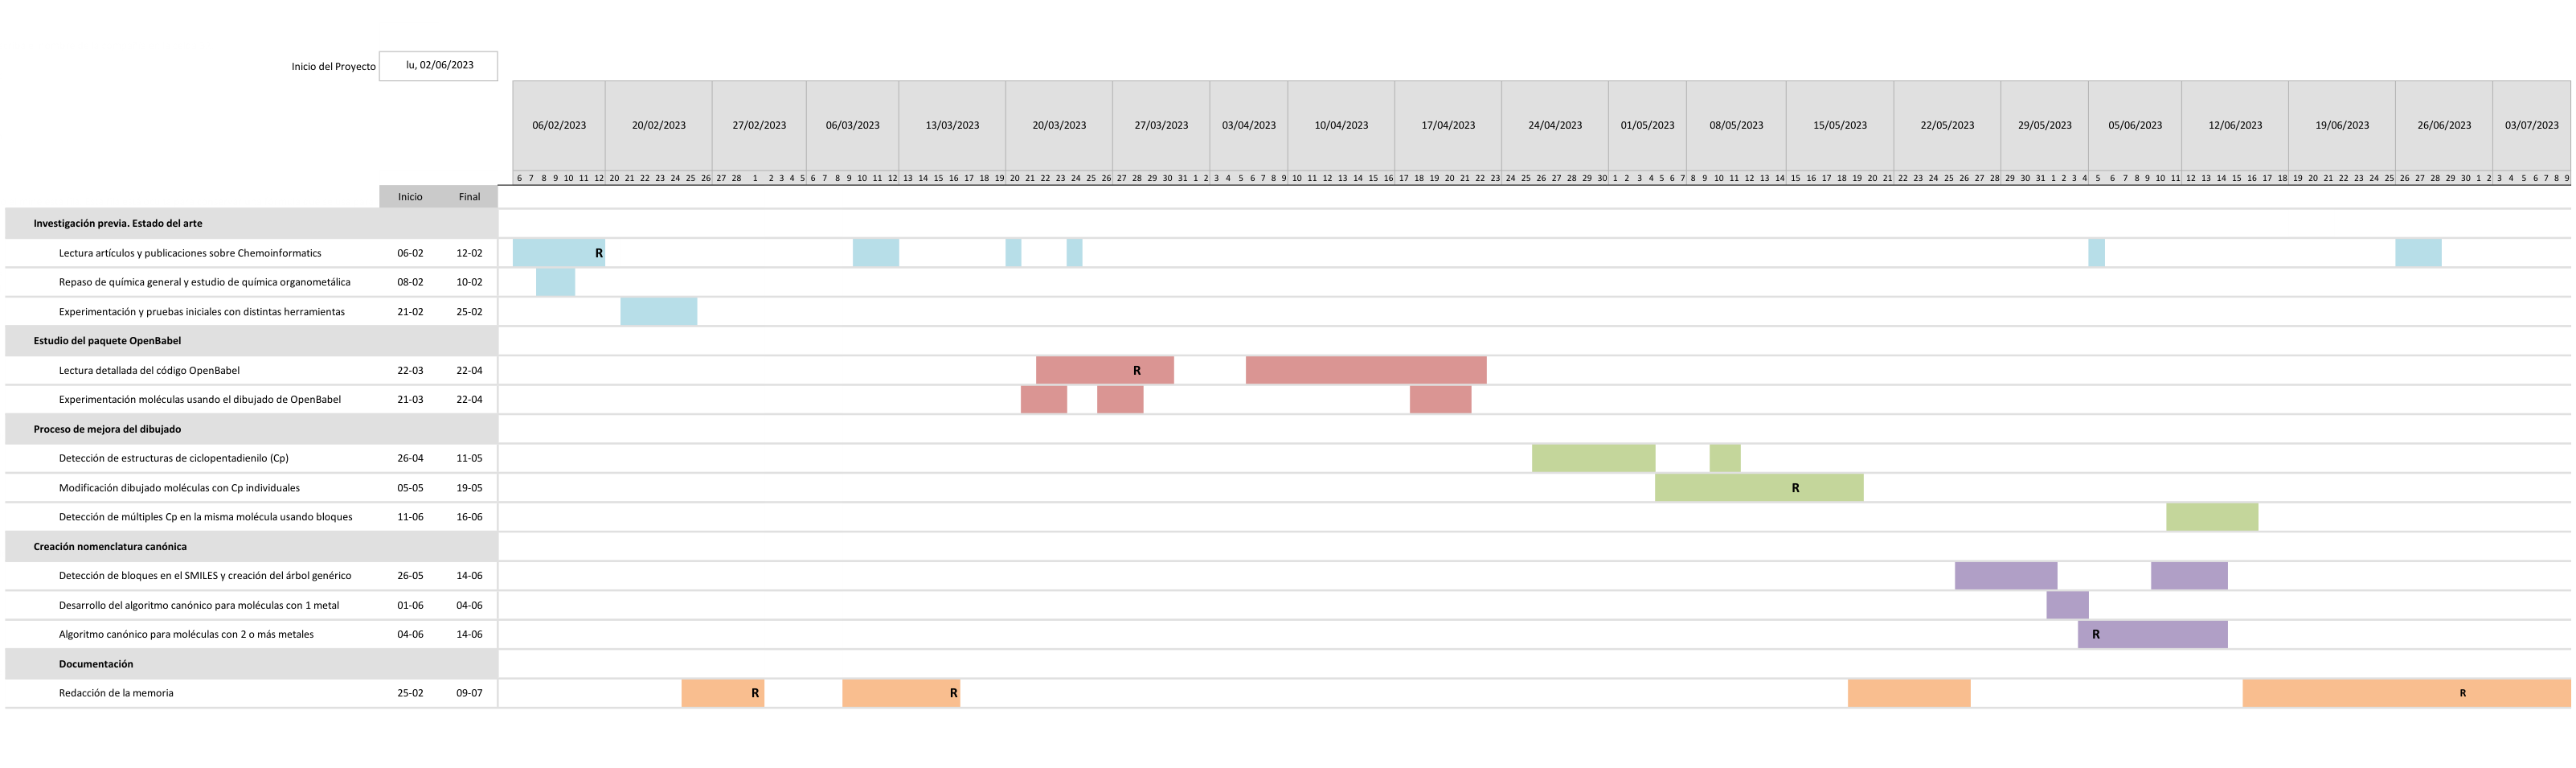
\includegraphics[scale=0.9]{imagenes/planificacion/planificacion_real.png}
        \caption{Diagrama de Gantt sobre la planificación temporal real}
        \label{fig:gantt_real}
    \end{figure}
\end{landscape}

% 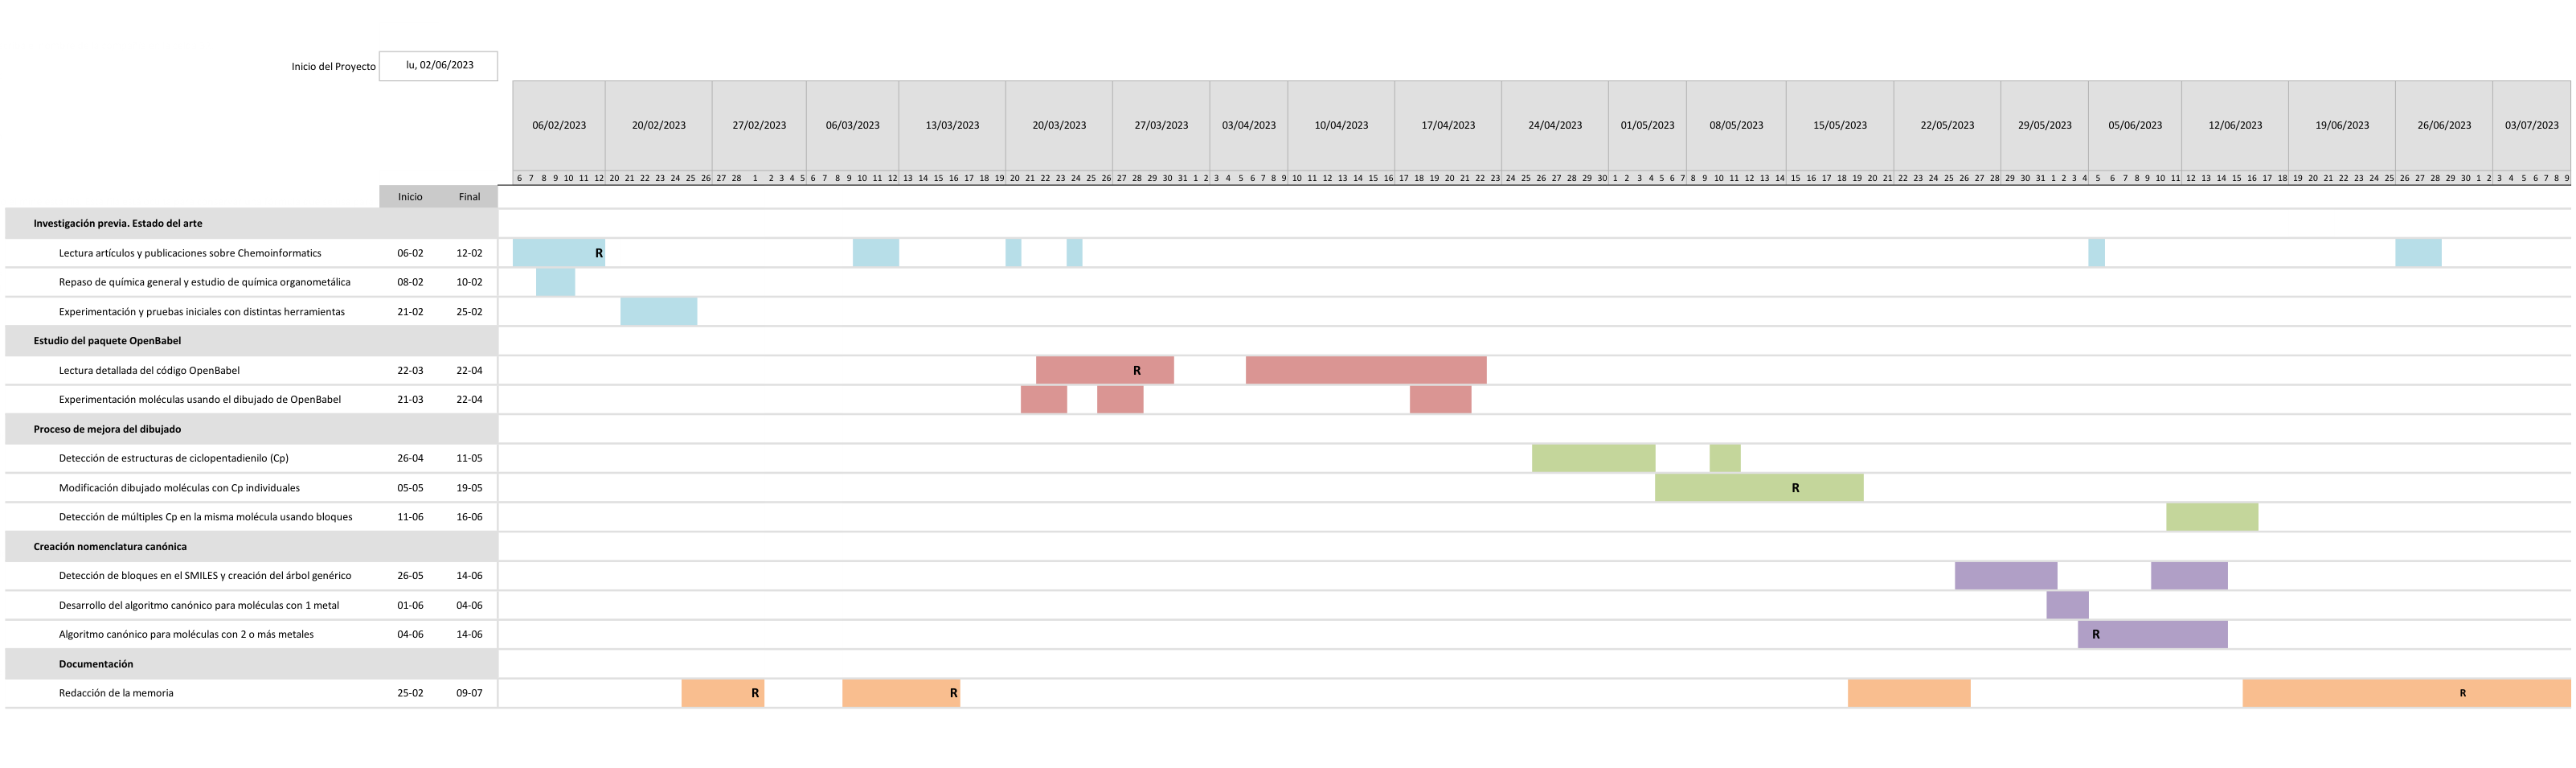
\includepdf[pages=-, offset=0 0,landscape=true,]{imagenes/planificacion/planificacion_real.png}


Como describo en la Sección \ref{riesgos_materializados}, el proceso de compresión del código base se alargó más de lo esperado, retrasando un poco el resto de tareas. En contraparte, la canonización y dibujado de las moléculas me llevó menos tiempo del estimado. Además, se invirtió el orden entre la modificación del sistema de dibujado y la creación del algoritmo de canonización con respecto a la planificación inicial. A priori era más sencillo alterar esa parte del código, y se podían obtener resultados más visuales.

\section{Gestión de la configuración}
En este apartado se describirá cómo se ha llevado a cabo la gestión de los activos de este proyecto, es decir, el código desarrollado y la documentación generada. Dado que son partes fundamentales del trabajo, atendiendo al análisis de riesgos descrito en la Sección \ref{riesgos} y el plan de actuación frente a la pérdida de información, se detalla a continuación la gestión de ambas.

\subsection{Gestión del código}
Para la gestión del código se ha usado un control de versiones a través de Git y Github. Ambas herramientas en conjunto permiten ir creando versiones intermedias del código conforme se va desarrollando y hacer copias de seguridad en la nube. También son muy útiles para proyectos colaborativos, donde varias personas del equipo pueden combinar fácilmente su parte del código desarrollado y revisar el progreso subido hasta el momento.
El procedimiento a seguir en la mayoría de casos es bastante similar. Se creará un repositorio remoto en la plataforma de GitHub con el nombre de \emph{TFG} —o el que uno prefiera— donde se irán almacenando los cambios\footnote{\url{https://github.com/Jesnm01/TFG}}. En la carpeta de trabajo local de nuestro computador, carpeta que contendrá en mi caso todos los elementos de los que quiera llevar un control, se creará un repositorio local usando Git, que habrá que vincular con el remoto para poder ir sincronizando los cambios. 


\subsection{Gestión de la documentación}
En lo relativo a la documentación, el proceso de gestión será similar ya que también se ha usado GitHub para su control de versiones. Esta se ha redactado en LaTeX usando el servicio online Overleaf. Overleaf cuenta con una opción para sincronizar el proyecto con un repositorio de GitHub, pero es una opción de pago. En su lugar, descargo el proyecto en el repositorio local y desde ahí ya realizo dicha sincronización para subir los cambios en el remoto.

Además, dada la naturaleza del proyecto y de la metodología de desarrollo utilizada, se ha llevado un registro de las reuniones con la tutora que también se ha ido actualizando periódicamente. Este documento pretende recoger los contenidos más relevantes de las reuniones: preguntas, comentarios, anotaciones, tareas que hacer, cosas pendientes de una reunión a otra, revisiones, y puntos a mejorar, entre otras cosas.



\section{Gestión de recursos} \label{gestion_recursos}

\subsection{Recursos humanos}
\begin{itemize}
    \item \textbf{Dña. Rocío Celeste Romero Zaliz}, profesora del Departamento de Ciencias de la Computación e Inteligencia Artificial de la Universidad de Granada en calidad de tutora del proyecto. A cargo de la supervisión y guía del alumno durante su desarrollo del trabajo.
    \item \textbf{Jesús Navarro Merino}, estudiante del grado en Ingeniería Informática en la Escuela Técnica Superior de Ingenierías Informática y Telecomunicación.
\end{itemize}


\subsection{Recursos materiales}
Para este proyecto no se han necesitado recursos adicionales, habiéndose usado únicamente los siguientes recursos materiales, ya existentes: 
\begin{itemize}
    \item \textbf{Portátil personal}: Portátil ACER Aspire A515-51G-8907 con un procesador Intel Core i7 8550U 1.8GHz, 20GB de memoria RAM y una arquitectura de 64 bits. Se ha usado durante todo el proyecto, para labores de programación y redacción de la memoria.
    \item \textbf{Pantalla}. Monitor utilizado de apoyo a la pantalla propia del portátil. De la marca AOC, de 24 pulgadas con una resolución de 1920x1080.
\end{itemize}


\subsection{Recursos software} \label{recursos_software}
En esta sección describiré todas aquellas herramientas software empleadas durante la realización del proyecto. Todas y cada una de ellas son herramientas de software libre, gratuitas o disponibles a través de licencias de estudiantado. A continuación se lista el software usado:
\begin{itemize}
    \item \textbf{Sistema operativo}: Windows 10 Home. Aunque por lo general Windows no es gratuito, al estar utilizando la típica licencia OEM que trae preinstalada el ordenador al comprarlo, la considero como tal.
    
    \item \textbf{Visual Studio C++}: es un IDE muy potente de Microsoft orientado a crear aplicaciones .NET y C++ para Windows. Se ha usado su versión gratuita Visual Studio Community 2022. Permite editar, depurar, realizar pruebas de testing, además de tener control de versiones integrado, entre otras cosas. Aquí se ha llevado a cabo todo el desarrollo del código.
    
    \item \textbf{OpenBabel}: Open Babel es una biblioteca de código abierto multiplataforma utilizada en química computacional y ciencias relacionadas para la conversión y manipulación de estructuras químicas en varios formatos. He trabajado con la versión 3.1.1 disponible en su repositorio de GitHub oficial\footnote{\url{https://github.com/openbabel/openbabel}}.

    \item \textbf{CMake}: es una herramienta de generación de archivos de compilación que simplifica el proceso de compilación y construcción de proyectos, permitiendo una configuración flexible e independiente de la plataforma. CMake utiliza archivos de configuración llamados CMakeLists.txt para describir la estructura del proyecto y las dependencias necesarias. Se ha usado en su versión 3.25.2 para la compilación y creación de soluciones de OpenBabel.

    \item \textbf{Git}: software de código abierto para el control de versiones de un proyecto.
    \item \textbf{Github}: es una plataforma donde se alojará el código y la documentación del proyecto. Utiliza Git por debajo y es una de las plataformas gratuitas para alojamiento de código mas empleadas a nivel mundial.

    \item \textbf{Google Colab}: es una plataforma en línea gratuita ofrecida por Google que permite a cualquier usuario escribir y ejecutar código en el navegador. Es una herramienta basada en la nube que proporciona un entorno de ejecución como si fueran notebooks de Jupyter, es decir, se puede escribir, editar y ejecutar código en bloques/celdas interactivos. Se ha usado durante las etapas iniciales del proyecto para la experimentación con diversas moléculas.
    
    \item \textbf{Zotero}: software de gestión de referencias bibliográficas que permite recopilar, organizar, citar y generar fácilmente una bibliografía en varios estilos de formato estándares según los documentos, páginas webs, artículos o archivos PDF guardados. Facilita la creación de referencias y citas en documentos académicos, ahorrando tiempo y asegurando un uso correcto de las fuentes consultadas.
    
    \item \textbf{Google Meet}: servicio de videoconferencias de Google. Plataforma utilizada para las reuniones con la tutora.

    \item \textbf{Google Drive Sync}: ahora llamada Google Drive para PC, es una aplicación de Google que permite sincronizar los archivos y carpetas de la computadora con la cuenta de Drive. Usado para realizar copias de seguridad —adicionales a lo almacenado en GitHub— de algunos archivos importantes. 

    \item \textbf{Overleaf}: herramienta online para la redacción de documentos en LaTeX usada para la documentación de este proyecto.

    \item \textbf{Scopus}: base de datos de referencias bibliográficas y citas de la empresa Elsevier.

    \item \textbf{Clockify}: herramienta online que te permite registrar las horas dedicadas a un proyecto.

    \item \textbf{Umbrello}: herramienta que combina funciones de modelado y generación de código para el lenguaje unificado de modelado (UML). Usado para la elaboración de los diagramas de clases.

    \item \textbf{Draw.io}: herramienta online para la creación de diagramas variados, esquemas y bocetos.

    \item \textbf{Correo UGR}: servicio de correo electrónico institucional de la UGR.

    \item \textbf{Microsoft Word}: procesador de textos de Microsoft usado para apuntes personales y documentación en sucio. Disponible a través de la cuenta de Microsoft Office 365 que ofrece la universidad.

    \item \textbf{Microsoft Excel}: utilizado para la creación de algunas tablas y gráficos incluidos en la memoria. Disponible a través de la cuenta de Microsoft Office 365 que ofrece la universidad.

    \item \textbf{Visual Studio Code y LaTeX}: VSCode es un editor de texto, que a través de algunas extensiones, permite editar, compilar y visualizar ficheros LaTeX. Es la alternativa a Overleaf según lo descrito en la Sección \ref{riesgos}. 

    
    
\end{itemize}

\section{Gestión de costes}
\textbf{TERMINAR esto cuando vaya acabando el trabajo}

En esta sección se realizará una estimación de los costes asociados al proyecto, atendiendo a los recursos descritos en la Sección \ref{gestion_recursos}. La elaboración de un presupuesto preciso en muchos casos puede suponer un desafío, ya que los proyectos software a menudo están sujetos a cambios y variables imprevistas, pero es una tarea importante para estudiar su viabilidad. 

\subsection{Coste de recursos humanos}
Si actuáramos como una empresa en un proyecto software al uso, existen muchos componentes que tener en cuenta para montar esta sección del presupuesto. Aspectos como el salario de los trabajadores y compensaciones varias, el coste de los procesos de selección y contratación, formación y desarrollo del personal, costes laborales adicionales (seguros, vacaciones, etc), o costes de personal externo (consultores o subcontratistas) entre otras cosas.
Dada la naturaleza de este proyecto, en relación a los gastos asociados a recursos humanos contamos con un equipo de desarrollo formado por una persona que tendrá el papel de Ingeniero Informático. Para estimar el costo de su trabajo, se indica el número total de horas dedicadas.

El intervalo de tiempo que está pensado para el proyecto son 5 meses, desde febrero hasta junio. 

\begin{center}
    $Dias\ totales\ =\ 5\ meses\ *\ 30\ dias / mes\ =\ 150\ dias$    
\end{center}

A este tiempo hay que descontarle los días no laborables de fines de semana más los días de vacaciones correspondientes por mes trabajado:

\begin{equation*}
    \textit{Dias no laborables} = \left( \frac{8 \textit{dias}}{mes} + \frac{22 \textit{ dias vacaciones}}{12 \textit{ meses}}\right) * 5 \textit{ meses} \approx 50 \textit{ dias}
\end{equation*}

Eso nos deja un total de 100 días aproximadamente de trabajo. Teniendo en cuenta una media semanal de 30 horas trabajadas repartidas en 6 horas diarias, tendríamos el siguiente total de horas trabajadas:
\begin{equation*}
    \textit{Horas trabajadas} = 100 \textit{dias} * 6 \textit{ horas/dia} = 600 \textit{ horas}
\end{equation*}

Esta cifra duplicaría la cantidad de horas que le corresponderían a un TFG según sus créditos asignados por la universidad. Estos cálculos como tal serían una estimación, pero se ha utilizado durante el desarrollo del proyecto la herramienta Clockify para el registro real de las horas dedicadas. Como se ve en la figura \ref{fig:clockify}, han sido \textbf{XXXXX} horas en total,
por lo que usaré ese dato para calcular el coste.

\begin{figure}[h!]
    \centering{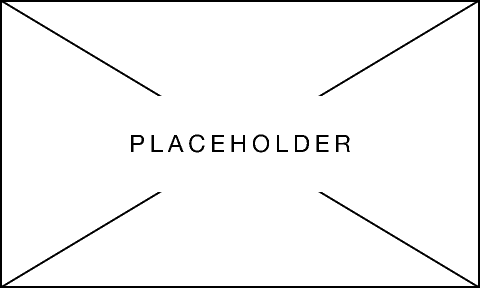
\includegraphics[scale=0.4]{imagenes/placeholder.png}}
    \caption{Registro de horas dedicadas al proyecto a través de Clockify}
    \label{fig:clockify}
\end{figure}

Según varias fuentes\footnote{\url{https://www.jobted.es/salario/ingeniero-informático}}\footnotecomma\footnote{\url{https://acortar.link/infojobs_salario}}\footnotecomma\footnote{\url{https://acortar.link/uax_salario}}, el salario medio de un ingeniero informático recién graduado está en torno a 21.000€. Siendo equivalente, unos 1750€ mensuales, que son 13,46€/hora. Con todo eso, tenemos que:
\begin{equation*}
    \textit{Coste total recursos humanos} = XXXX \textit{horas} * 13,46\EUR{}/hora = XXX \EUR{}
\end{equation*}


\subsection{Costes de recursos materiales}

Dado que no se han adquirido expresamente para este proyecto, ya que se poseían con anterioridad, no se valora su precio de compra como tal sino su valor de depreciación. Los productos electrónicos experimentan un proceso llamado depreciación, que conlleva una devaluación gradual a lo largo de su vida útil. Es importante tener esto en cuenta para estimar su valor actual y el coste del recurso. Esta estimación refleja el valor de un activo desde un punto de vista contable.

Al referirnos a la depreciación de un activo a lo largo de su vida útil, no se incluyen situaciones en las que sufra daños debido a accidentes, desastres naturales u otros eventos similares. En cambio, estamos hablando del desgaste del uso cotidiano, así como los impactos derivados de las innovaciones tecnológicas que surgen durante ese período que puedan dejar obsoleto el dispositivo.

Para calcular el valor actual de los activos utilizaré el método de depreciación lineal, que considera un desgaste uniforme durante su uso, mostrando el resultado del gasto anual de depreciación\cite{depreciacion_pcs}. Necesitamos lo primero, hallar el valor residual del activo, es decir, el valor que se estima que tendrá cuando llegue al final de su vida útil. Usaré para los dispositivos electrónicos una vida útil de 8 años. Haré un ejemplo con el coste del portátil.

\begin{equation*}
    \textit{Valor residual} = {\frac{\textit{Coste inicial}}{\textit{Vida util (años)}}} = \frac{689 \EUR{}} {8 \textit{ años}} = 86,125 \EUR{}
\end{equation*}

Con el valor residual estimado, se puede calcular la depreciación lineal anual con la siguiente fórmula.

\begin{equation*}
    \textit{Depreciación} = {\frac{\textit{Coste inicial} - \textit{Valor residual}}{\textit{Vida util (años)}}} = \frac{689\EUR{}-86,125\EUR{}} {8 \textit{ años}} = 75,36 \EUR{}
\end{equation*}

Teniendo estos 2 datos, se puede calcular el valor actual del activo teniendo en cuenta sus años de antigüedad. Se muestran todos los datos relativos a los costes materiales en la Tabla \ref{tabla:costes_materiales}.


\begin{table}[ht]
\small
    \begin{tabular}{lllll}
    \toprule 
    % Al parecer tengo que hacer esto asi tan extraño (meter una tabla de 1 celda dentro de la propia celda para poder meter un salto de linea...)
    \textbf{Recurso} & \textbf{\begin{tabular}[c]{@{}l@{}}Valor\\ inicial (€)\end{tabular}} & \textbf{\begin{tabular}[c]{@{}l@{}}Depreciación\\ anual (€)\end{tabular}} & \textbf{\begin{tabular}[c]{@{}l@{}}Antigüedad\\ (años)\end{tabular}} & \textbf{\begin{tabular}[c]{@{}l@{}}Valor\\ actual (€)\end{tabular}} \\ 
    \midrule
    Portátil personal           & 689 & 75,36 & 5 & 312,2         \\ 
    Pantalla AOC                & ~230 & 25,15 & 2 & 179,69         \\ 
    \midrule
    \multicolumn{4}{r}{\textbf{Total:} } & 491,89 \\
    \bottomrule
\end{tabular}
\caption{Tabla de los costes materiales}
\label{tabla:costes_materiales}
\end{table}

\subsection{Costes software}
Los costes relacionados con los recursos software son nulos. Como indico en el listado de recursos de la Sección \ref{recursos_software}, son herramientas de software libre, utilizadas mediante licencias gratuitas o mediante acceso vía instituciones autorizadas como la UGR, por lo que no suponen coste alguno en el desarrollo de este proyecto.

\subsection{Otros costes}
Aquí se incluyen todos los demás gastos que han sido necesarios para el desarrollo del proyecto y que no pertenecen a los apartados anteriores. Principalmente son los gastos vinculados a las facturas de la luz e Internet. El coste de la tarifa de Internet contratada es de 40€/mes, que a lo largo de los 5 meses el total asciende a 200€. Para la luz, una estimación posible serían 19,58€, teniendo en cuenta el gasto que suponen los recursos materiales en base a una factura trimestral de 11,80€.

\begin{table}[ht]
    \centering
    \begin{tabular}[t]{lc}
        \toprule
        \textbf{Recursos} & \textbf{Importe (€)}  \\
        \midrule
        Luz         &   19,58   \\
        Internet    &   200      \\
        \bottomrule
    \end{tabular}
    \caption{Tabla de costes adicionales}
    \label{tabla:costes_adicionales}
\end{table}




\subsection{Presupuesto final}
Se presenta por tanto el presupuesto completo asociado al proyecto, dividido en cada una de las secciones tratadas anteriormente. Se ve el desglose en la Tabla \ref{tabla:presupuesto_total}.
\begin{longtable}[c]{lm{2cm}r}
\toprule
\textbf{Detalle}                        && \textbf{Importe} \\
\endfirsthead
%
\endhead
%
% \hline
\endfoot
%
\endlastfoot
%
\midrule
                                        % &                 \\\hline
\textbf{Costes de recursos humanos}     && \textbf{X €} \\
Trabajo autónomo                        && X €          \\
\midrule
\textbf{Costes de recursos materiales}  && \textbf{491,89 €} \\
Portátil personal                       && 312,2 €            \\ %Esto para darle un tabulado al elemento
Pantalla de apoyo                       && 179,69 €             \\ 
\midrule
\textbf{Costes de recursos software}    && \textbf{0,00 €}    \\
                                        % & \multicolumn{1}{l}{}    \\
Windows 10                              && 0,00 €             \\
Visual Studio C++                       && 0,00 €             \\
OpenBabel                               && 0,00 €             \\
CMake                                   && 0,00 €             \\
Git                                     && 0,00 €             \\
GitHub                                  && 0,00 €             \\
Google Colab                            && 0,00 €             \\
Zotero                                  && 0,00 €             \\
Google Meet                             && 0,00 €             \\
Google Drive Sync                       && 0,00 €             \\
Overleaf                                && 0,00 €             \\
Scopus                                  && 0,00 €             \\
Clockify                                && 0,00 €             \\
Draw.io                                 && 0,00 €             \\
Correo UGR                              && 0,00 €             \\
Microsoft Word                          && 0,00 €             \\
Microsoft Excel                         && 0,00 €             \\
Visual Studio Code y LaTeX              && 0,00 €             \\
\midrule
\textbf{Costes adicionales}             && \textbf{219,58 €}  \\
                                        % & \multicolumn{1}{l}{}                   \\
Internet                                && 40€ x 5 meses = 200€           \\
Factura de la luz                       && 19,58 €            \\
                                        % & \multicolumn{1}{l}{}                   \\
\midrule
  &   \multicolumn{1}{r}{\textbf{Total:}} & \textbf{X €} \\
\bottomrule
\caption{Presupuesto total del proyecto}
\label{tabla:presupuesto_total}
\end{longtable}


\section{Análisis de riesgos} \label{riesgos}
El análisis de riesgos desempeña un papel fundamental en la planificación y ejecución exitosa de proyectos. A veces surgen imprevistos que pueden afectar en mayor o menor medida a la correcta evolución de estos. Por ello, la aplicación de este proceso resulta esencial para minimizar la incertidumbre, intentar evitar la aparición de esos riesgos, y en caso de que se materialicen, paliarlos o mitigarlos de manera efectiva mediante unos planes de actuación.

En este aparatado por tanto, se analizarán los riesgos potenciales del proyecto, incluyendo sus causas y el plan de acción para resolverlos o mitigar su impacto al máximo (Figura \ref{tabla:tabla_riesgos}). Además, se realizará una evaluación de la probabilidad de ocurrencia y del impacto asociado a cada riesgo, que se puede ver en la Figura \ref{tabla:riesgos_matriz_probabilidad}. Esto se basa en una matriz con 2 dimensiones: la probabilidad de ocurrencia de un riesgo y el impacto que tendría en el proyecto si se materializa. Se valorarán los riesgos según aspectos técnicos, de recursos humanos o complejidad y naturaleza del proyecto, y preguntas del tipo, ¿qué tan difícil sería recuperarse del riesgo?, ¿cuál es el resultado más negativo que podría originarse como consecuencia? o ¿ha sucedido este riesgo o alguno similar anteriormente?

\begin{figure}
    \centering
    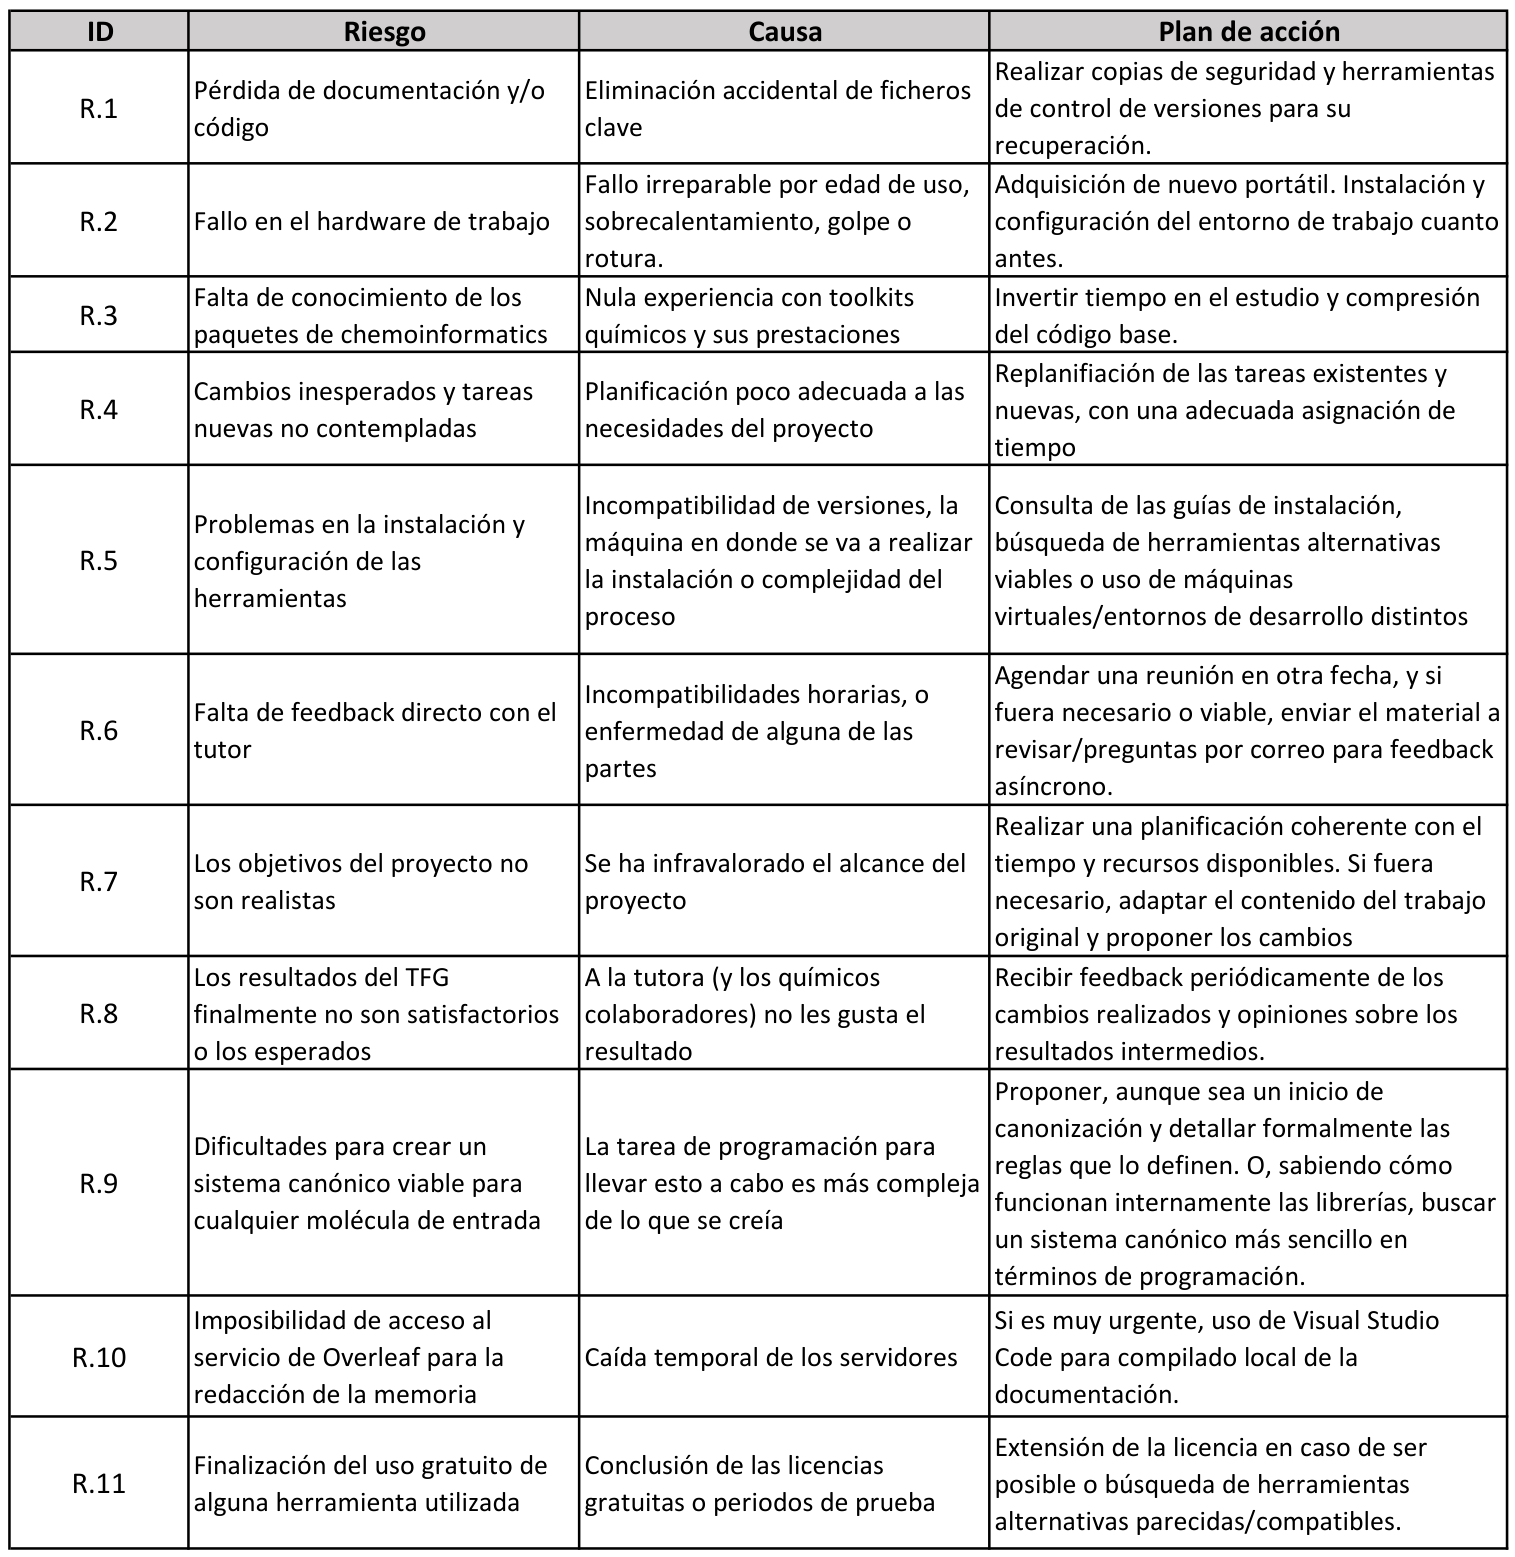
\includegraphics[scale=1]{imagenes/planificacion/riesgos-1_cropped.png}
    \caption{Riesgos del proyecto, causas, y planes de actuación}
    \label{tabla:tabla_riesgos}
\end{figure}

\begin{figure}
    \centering
    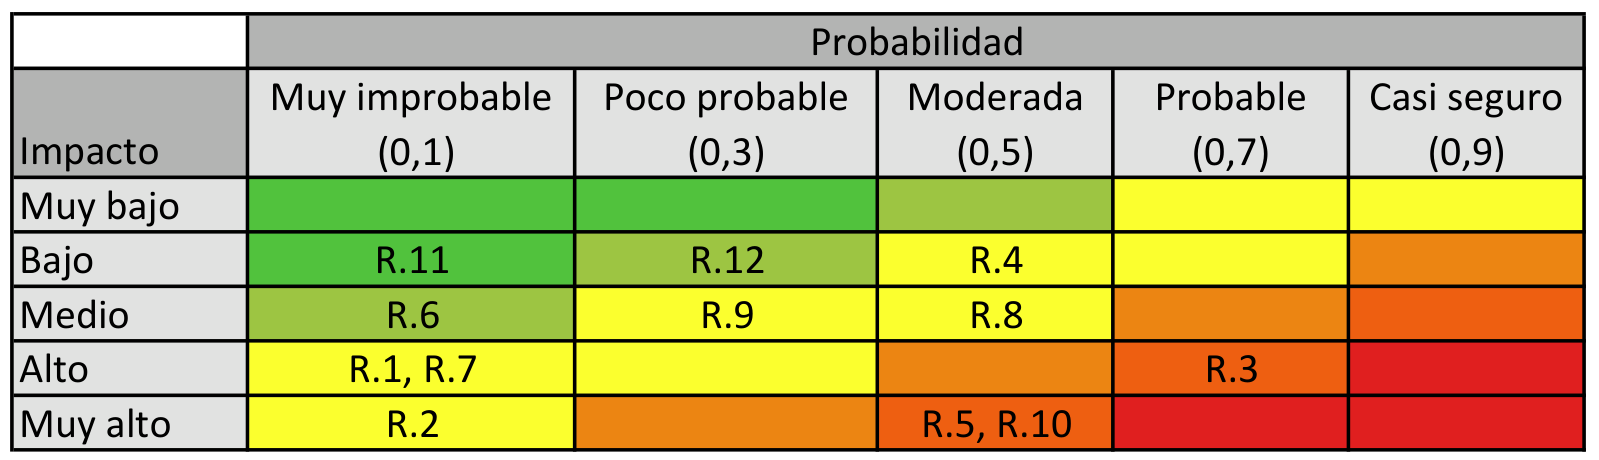
\includegraphics[scale=0.95]{imagenes/planificacion/matriz_riesgos.png}
    \caption{Matriz de probabilidad-impacto de riesgos}
    \label{tabla:riesgos_matriz_probabilidad}
\end{figure}

\subsection{Riesgos materializados}\label{riesgos_materializados}

\textbf{completar esto al final del trabajo, o conforme se vayan ocurriendo}


Los riesgos materializados han estado relacionados principalmente con aspectos técnicos. Primeramente, el R.5. Tuve problemas para instalar OpenBabel en mi máquina por problemas de versiones, por lo que acabé utilizando Google Colab como entorno virtual e instalar ahí algunas librerías necesarias para las primeras experimentaciones con moléculas. Esto tampoco era muy útil a largo plazo puesto que tenía que poder acceder al código fuente para modificarlo, añadir las funcionalidades y compilarlo manualmente para probar los cambios. Por lo que finalmente con ayuda de las guías, se pudo ejecutar localmente. Instantáneamente después, se materializó el riesgo R.3. La falta de conocimiento ante una librería tan grande ya existente retrasó considerablemente el proceso de modificación del código. 
\textbf{Añadir mas riesgos conforme se vayan materializando}

Finalmente, se consiguieron solventar los riesgos manifestados mediante los planes de actuación descritos en cada uno de ellos.


\chapter{Diseño e implementación}

En este capítulo se describirán las clases y todos los métodos que se han añadido y modificado durante el proceso de implementación a partir del código base de OpenBabel en su versión 3.1.1 (disponible en su repositorio oficial de GitHub\footnote{\url{https://github.com/openbabel/openbabel/releases}}). OpenBabel está escrito en C++, por lo que el proceso de desarrollo se ha llevado a cabo exclusivamente en este lenguaje, usando para ello el IDE \textit{Visual Studio C++} para Windows.


\section{Diseño}

\subsection{Estructura de OpenBabel}

A partir del código fuente de OpenBabel, al compilar los archivos fuente y generar el proyecto, los archivos de configuración de CMake generan una serie de \emph{soluciones}. Hay soluciones que consisten únicamente en el archivo `\textit{main}', que representa el ejecutable al que llamamos por línea de órdenes desde la terminal. El resto de soluciones forman la propia API de OpenBabel, siendo las clases más importantes `\textit{OBMol}', `\textit{OBAtom}', y `\textit{OBBond}', que permiten almacenar la información de una molécula, un átomo, o un enlace entre átomos respectivamente; y otras clases más orientadas a la conversión entre formatos como `\textit{OBConversion}' u `\textit{OBFormat}'. De entre ellas la clase central es OBMol, que almacena toda la información básica relacionada con una molécula, incluyendo la lista de átomos, la lista completa de enlaces entre átomos, identificadores de cada átomo y enlaces y entre otras variables, el vector de coordenadas 2D de todos los átomos para su representación gráfica.

A continuación se muestra la estructura general de directorios de OpenBabel:
\vspace{0.5cm}
\dirtree{%
.1 openbabel-3-1-1/.
    .2 cmake/\DTcomment{\textit{algunos ficheros de configuración para cmake}}.
    .2 data/\DTcomment{}.
    .2 doc/\DTcomment{\textit{documentación del proyecto y ficheros para su generación automática}}.
    .2 include/\DTcomment{\textit{ficheros .h}}.
        .3 openbabel/.
            .4 depict/\DTcomment{\textit{representación de moléculas}}.
            .4 math/.
            .4 stereo/.
            .4 tree/.
            .4 clases principales de Openbabel.
                .5 ....
    .2 src/\DTcomment{\textit{ficheros .cpp}}.
        .3 charges/.
        .3 depict/\DTcomment{\textit{representación de moléculas}}.
        .3 descriptors/.
        .3 fingerprints/.
        .3 formats/\DTcomment{\textit{soporte para distintos formatos de conversión}}.
        .3 math/.
        .3 ops/\DTcomment{\textit{plugins de la comunidad}}.
        .3 stereo/.
        .3 clases principales de Openbabel.
            .4 ....
    .2 scripts/\DTcomment{\textit{bindings para usar la interfaz en otros lenguajes}}.
    .2 test/\DTcomment{\textit{ficheros de ejecución de tests y datos de prueba}}.
    .2 tools/\DTcomment{\textit{\textit{`mains'} para ejecución por línea de órdenes}}.
    .2 CMakeLists.txt\DTcomment{\textit{archivo principal de configuración de cmake}}.
    .2 INSTALL\DTcomment{\textit{instrucciones breves de instalación de openbabel}}.
    .2 ficheros propios de .git\DTcomment{}.
}


\subsection{Diagrama de Clases}

 En el siguiente Diagrama de clases (Figura \ref{fig:diagrama_clases}) se muestran tanto las clases que se han visto modificadas (en color anaranjado), las creadas desde cero (en color más verdoso) y las demás clases importantes que interactúan con las anteriores pero no se han visto alteradas (en amarillo). 

\begin{landscape}

    \begin{figure}[]
        \centering
        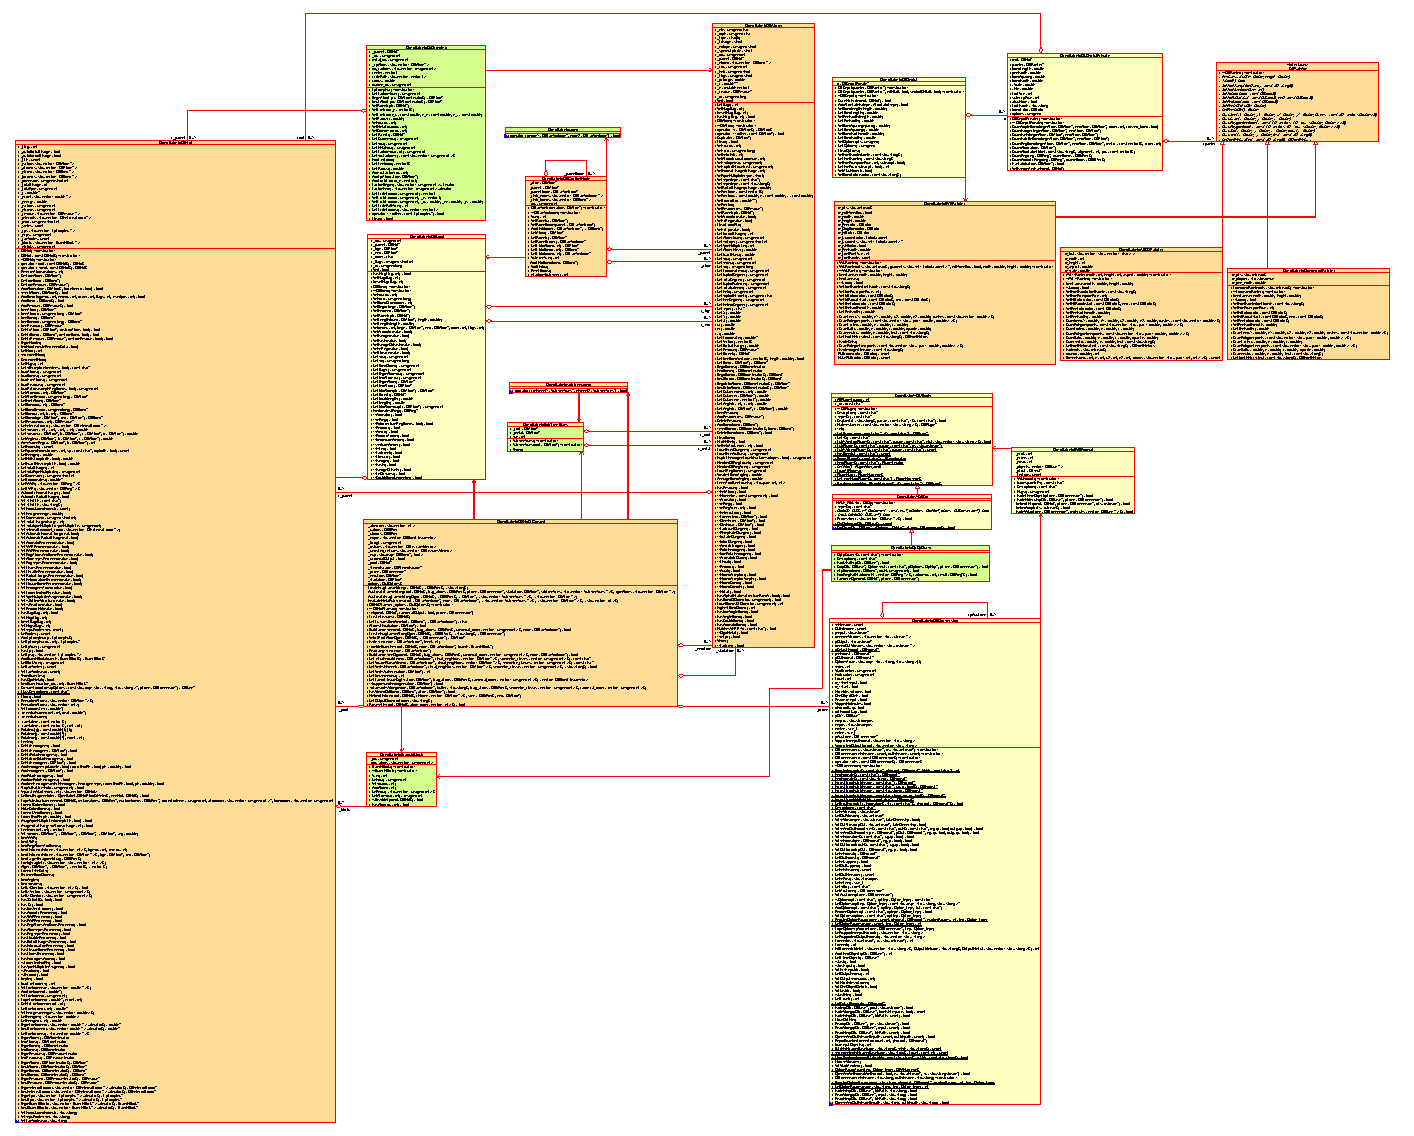
\includegraphics[scale=0.7]{imagenes/diseno/diagramaClasesHorizontal_cropped.pdf}
        \caption{Diagrama de clases}
        \label{fig:diagrama_clases}
    \end{figure}
\end{landscape}

% 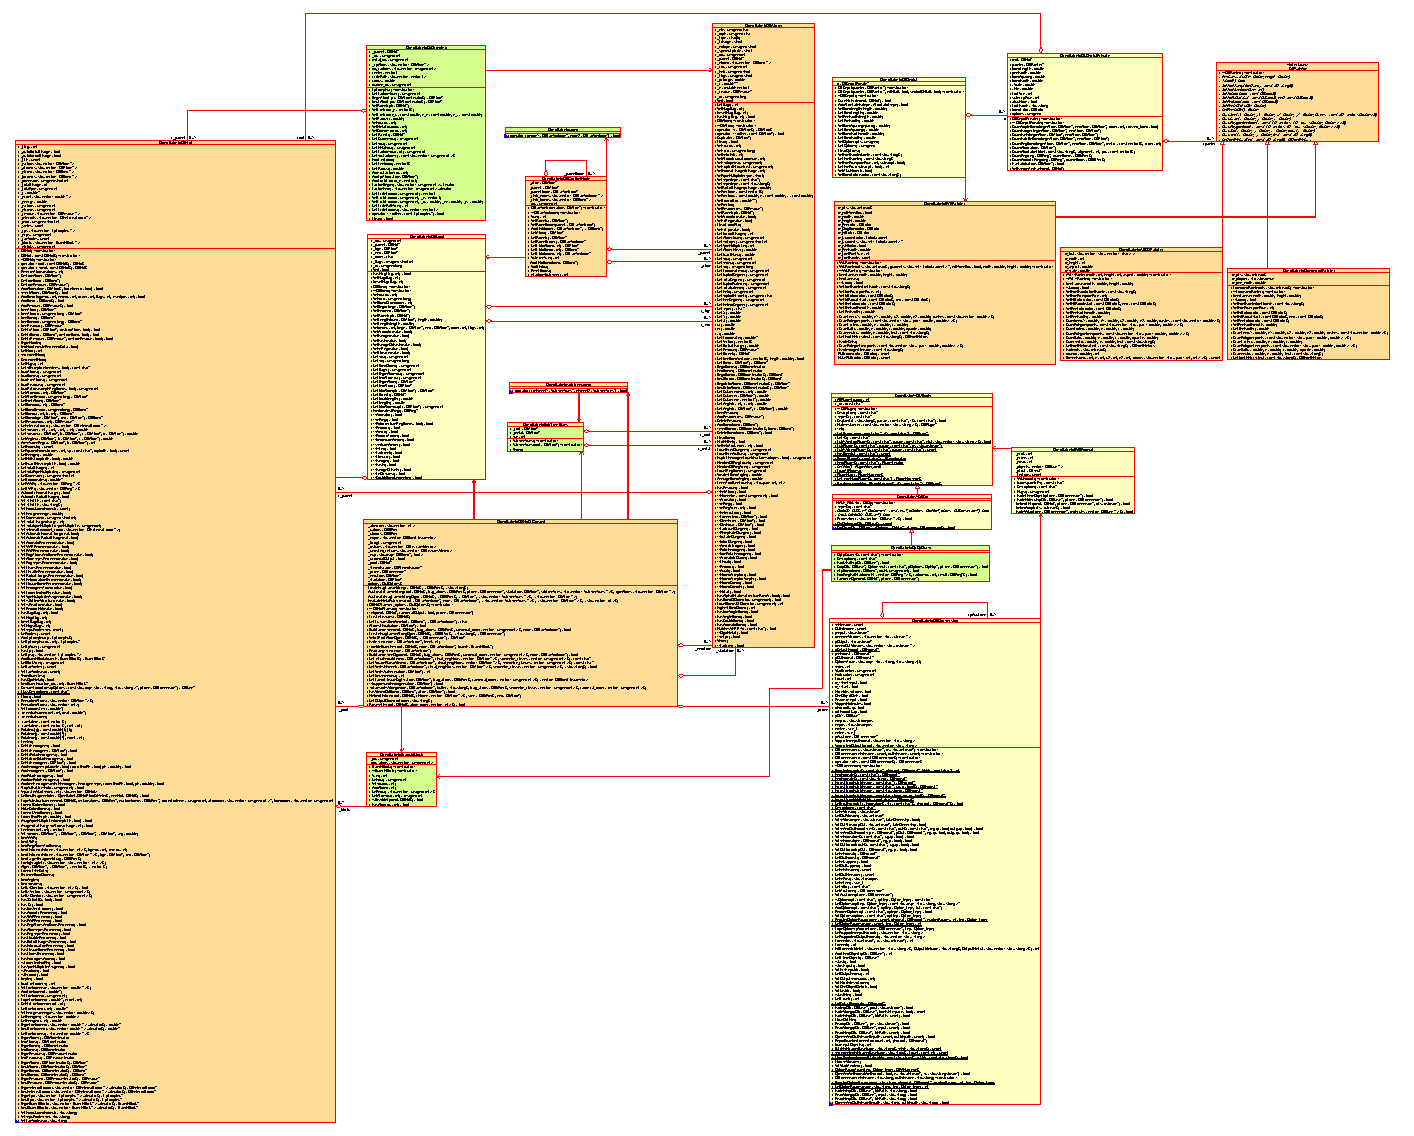
\includepdf[pages=-, offset=0 0,landscape=true,]{imagenes/diseno/diagramaClasesHorizontal_cropped.pdf}


Se pasa a detallar ahora cada una de las clases, tanto las modificadas como las nuevas, para qué sirven, y en qué consisten sus métodos. Las clases que no se han alterado, al igual que el resto de clases que no se incluyen en el diagrama se puede consultar su documentación en la página oficial\footnotemark. Puntualizar que existe una enorme cantidad de clases en la librería de OpenBabel, no tendería sentido añadirlas todas en el diagrama. Además, no todas poseen de documentación, por lo que la mayoría no aparecerán en\footnote[1]{\url{https://openbabel.github.io/api/3.0/index.shtml}}.


%  ------------------------- Cabeceras -------------------------
\subsection{Clases modificadas}
\begin{itemize}
    \item \textbf{OBPainter}: clase base abstracta para las clases de representación gráfica 2D (en \textit{/depict/painter.h}). Se ha añadido el siguiente método para poder utilizarlo en las clases que implementan esta interfaz:
    \begin{lstlisting}[language=C++]
        public: 
    
virtual void DrawPolygonLine(const std::vector<std::pair<double, double> >& points) = 0;
    \end{lstlisting}

    \item \textbf{SVGPainter}: clase que hereda de OBPainter y genera representaciones 2D en el formato de gráficos vectoriales SVG (en \textit{/depict/svgpainter.h}).
    \begin{lstlisting}[language=C++]
        public: 
    
//Inserts the necessary xml code in the .svg output file to draw a polygon according to the vector of points specified by @p points
void DrawPolygonLine(const std::vector<std::pair<double, double> >& points);
    \end{lstlisting}

    \item \textbf{ASCIIPainter}: clase que hereda de OBPainter (en \textit{/depict/asciipainter.h}).
    \begin{lstlisting}[language=C++]
        public: 
    
//The method is declared empty to avoid compilation errors due to interface implementation. It has no use 
void DrawPolygonLine(const std::vector<std::pair<double, double> >& points);
    \end{lstlisting}

    \item \textbf{CommandPainter}: clase que hereda de OBPainter (en \textit{/depict/commandpainter.h}).
    \begin{lstlisting}[language=C++]
        public: 
    
//The method is declared empty to avoid compilation errors due to interface implementation. It has no use 
void DrawPolygonLine(const std::vector<std::pair<double, double> >& points);
    \end{lstlisting}

    % -------------------------- Atom ---------------------------
    \item \textbf{OBAtom}: clase principal, contiene la información relativa a un átomo, guardando su número atómico, cantidad de hidrógenos implícitos, una lista de los enlaces de este átomo con los demás y el vector de coordenadas 2D para su representación, entre otras variables (en \textit{/openbabel/atom.h}). Se han añadido los siguientes métodos:
    \begin{lstlisting}[language=C++]
class OBAPI OBAtom: public OBBase{
    public: 
    
//\return Is this a metal commonnly present in organometallic compounds?
bool IsOgmMetal();

//\return Is atom part of a Cp ring?
bool IsInCp() const;

//\return Is this atom a Carbon (atomic number == 6)?
bool IsCarbon();

//Debug method. Displays on basic output simple data to identify the atom
void Show();

//Mark an atom as part of a Cp ring
void SetInCp(bool value = true);

//! \return A pair<bool, idx> whether this atom has a bond with a metal atom. If true, also returns metal idx
std::pair<bool, int> HasOgmMetalBond();
};//class
    \end{lstlisting}


    % -------------------------- Mol ---------------------------
    \item \textbf{OBMol}: clase principal, almacena toda la información básica relacionada con una molécula. Esto incluye la lista de átomos, la lista completa de enlaces entre átomos, identificadores de los átomos y enlaces, y el vector de coordenadas 2D de todos los átomos para su representación entre otras variables (en \textit{/openbabel/mol.h}). Se han añadido las siguientes variables y métodos:
    \begin{lstlisting}[language=C++]
class OBAPI OBMol: public OBBase {
    private: 
    
std::string _smiles;                //!< Input smiles string for the molecule
std::vector<CpComplex*> _cps;       //!< Cp information
unsigned int _ncps;                 //!< Number of cps complexes detected
std::string  _canSmiles;            //!< Canonical smiles based on Ogm canonicalization
std::vector<BranchBlock*> _blocks;  //!< Branches information
unsigned int _nblocks;              //!< Number of blocks


    public: 
    
//! Set the input smiles string of this molecule to @p smi
void SetInputSmiles(std::string smi);

//! \return the input smiles string of this molecule
std::string GetSmiles();

//! Add a new CpComplex specified by @p cp
void AddCpComplex(CpComplex& cp);

//! \return the cp at index @p idx or NULL if none exists.
CpComplex* GetCpComplex(int idx);

//! \return number of cp in the molecule
unsigned int GetCpSize();

//! \return whether the molecule has cps or not
bool HasCp();

//! \return the whole container of cps of this molecule
std::vector<CpComplex*> GetCps();

//! Add a new block to the molecule, specified by @p branch
BranchBlock* AddBranchBlock(BranchBlock& branch);

//! \return the number of blocks in the molecule
unsigned int GetBlockSize();

//! \return the canonical smiles string generated by the ogm canonicalization methods
std::string GetCanSmiles();

//! Set the canonical smiles string of this molecule to @p smi
void   SetCanSmiles(std::string smi);

//! Debug method. Displays on basic output all molecule blocks with basic information of the atoms.
void ShowBranches();

//! \return If this molecule has any Ogm metal or not
bool HasOgmMetal();

//! \return the block of which the carbon at index @p carbon_idx is part, or NULL if no such block exists
BranchBlock* FindBranch(int carbon_idx);

//! Set the iterator to the beginning of the Cp list
//! \return the first Cp structure, or NULL if none exist
CpComplex* BeginCp(std::vector<CpComplex*>::iterator & i);

//! Advance the iterator to the next Cp record
//! \return the next first Cp record, or NULL if none exist
CpComplex* NextCp(std::vector<CpComplex*>::iterator& i);

//! Set the iterator to the beginning of the BranchBlock list
//! \return the first BranchBlock structure, or NULL if none exist
BranchBlock* BeginBranchBlock(std::vector<BranchBlock*>::iterator& i);

//! Advance the iterator to the next BranchBlock record
//! \return the next first BranchBlock record, or NULL if none exist
BranchBlock* NextBranchBlock(std::vector<BranchBlock*>::iterator& i);
};//class
    \end{lstlisting}


    % -------------------------- OBMol2Cansmi ---------------------------
    \item \textbf{OBMol2Cansmi}: clase que maneja la conversión del smiles de entrada a un smiles canónico (en \textit{src/formats/smilesformat.h}). Se han añadido los siguientes métodos:
    \begin{lstlisting}[language=C++]
class OBMol2Cansmi{
        private: 
    
//Only changed visibility to private, since CreateFragCansmiStringOgm was created. Selects the "root" atom, which will be first in the SMILES, then builds a tree in canonical order, and finally generates the SMILES.
void CreateFragCansmiString(OBMol&, OBBitVec&, std::string&);

    
//Auxiliary private methods for SelectRootAtomOgm

//Shortened version of the CreateCansmiString method. Create the necessary variables to call AuxCreateFragCansmiStringOgm.
void AuxCreateCansmiString(OBMol& mol, OBBitVec& frag_atoms, OBConversion* pConv, OBAtom* startatom, std::vector<SubTreeSizes*>& subtreeSizes, std::vector<OBAtom*> ogmAtoms);

//Shortened version of the CreateFragCansmiStringOgm method. Create the necessary variables to build a new canonical tree using as root @p startAtom
void AuxCreateFragCansmiStringOgm(OBMol&, OBBitVec&, OBAtom*, std::vector<SubTreeSizes*>&, std::vector<OBAtom*>);

//Once the tree is built, this method runs through it in DFS evaluating the subtrees hanging from the other ogm metals. Use the auxiliary struct SubTreeSizes for this. 
void EvaluateMetalSubTrees(OBCanSmiNode* root, OBCanSmiNode* node, std::vector<SubTreeSizes*>&, std::vector<OBAtom*>&, std::vector<int>&);

        public: 
//Method based on CreateFragCansmiString. Share much of the code, with some additional methods specifically for my own canonical form designed for organometallic molecules.
void CreateFragCansmiStringOgm(OBMol&, OBBitVec&, std::string&, OBConversion*);

//If more than 1 Ogm metal is present in the molecule, this method chooses one of them, based on some rules and the conectivity of the metal within the molecule and the rest of the atoms
OBAtom* SelectRootAtomOgm(OBMol&, OBConversion*);

//Debug method for writing in basic output the tree with hierarchy formating
void WriteTree(OBCanSmiNode* node, int level = 0);

//Adds information to the molecule of the blocks that form it. Being a block, each set of atoms that, due to their bonds, are within the same parenthesis in the original input Smiles. Or, according to the OBMol2Cansmi::BuildCanonTree method, the parent-child relationship between atoms.
void IdentifyBranches(OBMol& mol,OBCanSmiNode* node, BranchBlock* branch = nullptr);

//Modifies the tree built by BuildCanonTree based on the length of the branches identified in IdentifyBranches. This is a canonical rule designed for a little more consistency in the output canon smiles.
void RearrangeTree(OBCanSmiNode* node);

//Builds the SMILES tree, in canonical order, for the specified molecular fragment. Based on the BuildCanonTree method. Shares much of the code, with some changes in the neighbour selection algorithm.
bool BuildCanonTreeOgm(OBMol& mol, OBBitVec& frag_atoms, vector<unsigned int>& canonical_order, OBCanSmiNode* node);
};//class
    \end{lstlisting}


    % -------------------------- OBCanSmiNode ---------------------------
    \item \textbf{OBCanSmiNode}: clase que representa un nodo. En conjunto se forma una estructura de árbol, cada nodo es un átomo del árbol para luego escribir el SMILES canónico (en \textit{src/formats/smilesformat.h}). Se han añadido los elementos:
    \begin{lstlisting}[language=C++]
class OBMol2Cansmi{
        private: 
    
OBCanSmiNode* _parentNode;      //!< Pointer to the parent node

//! Add a child bond to the node, specified by @p bond. Should only be used in the ResetBonds method as a part of the OBMol2Cansmi::RearrangeTree algorithm.
//! Otherwise, use addChildnode to add both the child node and its respective bonds
void AddChildBond(OBBond* bond);

        public: 

//! Set the parent node to @p parent
void SetParentNode(OBCanSmiNode* parent);

//! \return the parent node
OBCanSmiNode* GetParentNode();

//! Traverses the tree in dfs from the node calling the method
//! \return the number of total children (counting himself) 
int SubTreeSize();

//! Sort a node's child_nodes using a std::sort operation an a custom comparator 'mycomp'
void SortChilds();

//! When added at the same time in the addchildnode method, the child with its bond have a 1 to 1 index correspondence. When reordering the children, in OBMol2Cansmi::RearrangeTree, the indices of the bonds are lost. This method clears and adds the bonds back in order.
void ResetBonds();

//! \return the total number of carbons in this node subtree
int nCarbonsSubTree();
};//class
    \end{lstlisting}

\end{itemize}





\subsection{Clases nuevas}
\begin{itemize}
    % -------------------------- CpComplex ---------------------------
    \item \textbf{CpComplex}: nueva clase principal que maneja y permite almacenar estructuras de ciclopentadienilo (en \textit{/openbabel/cpcomplex.h}). Se han creado las siguientes variables y métodos:
    \begin{lstlisting}[language=C++]
class CpComplex {
	protected:
  
OBMol* _parent;                         //!< Parent molecule
unsigned int _idx;                      //!< Cp identifier within the molecule
unsigned int metal_idx;                 //!< Atom idx of central metal
std::vector<OBAtom*> _cpAtoms;          //!< Atoms for the carbons of the Cp structure
std::vector<unsigned int> idx_carbons;  //!< Atom indexes for the carbons of the Cp structure
vector3 center;                         //!< Cp center, for normal bond connection with metal atom, and aromatic circle position
std::vector<vector3> circlePath;        //!< Coordinates for the cp circle (needed to achieve a perspective circunference)
double radius;                          //!< Cp's aromatic circle radius
unsigned int dummy_idx;                 //!< Dummy central atom idx


        public:

//! Default constructor 
CpComplex();

//! \name Methods to modify internal information
//@{
//! Attach an OBMol @p ptr as the parent container for this Cp
void SetParent(OBMol* ptr);
//! Set the center point of the Cp, sprecified by @p _v. It is equidistant to every carbon in th Cp, as they are disposed in a regular polygon
void SetCentroid(vector3& _v);
//! Set the center point of the Cp, sprecified by @p v_x, v_y, v_z. It is equidistant to every carbon in th Cp, as they are disposed in a regular polygon
void SetCentroid(const double v_x, const double v_y, const double v_z);
//! Set the radius of the Cp circle
void SetRadius(double r);
//! Set the Cp identifier
void SetIdx(int idx);
//! Set the idx of the central metal to which this Cp is attached
void SetMetalIdx(int midx);
//! Dummy atom is created to make a perpendicular bond between the metal and the Cp drawing
//! Set the atom idx of the dummy atom created for this Cp 
void SetDummyIdx(int idx);
//! Set the point of the Cp circle at index @p i to the coordinates specified by @p _v
void SetCircleCoord(unsigned int i, vector3 _v);
//! Set the point of the Cp circle at index @p i to the coordinates specified by @p _vx, _vy, _vz
void SetCircleCoord(unsigned int i, double _vx, double _vy, double _vz = 0.0);
//@}


//! \name Methods to retrieve information
//@{
//! \return number of carbon atoms in the cp
unsigned int GetCarbonsSize();
//! \return the molecule which contains this Cp, or NULL if none exists
OBMol* GetParent();
//! \return dummy atom idx for this Cp structure, or 0 if none exists
unsigned int GetDummyIdx() const;
//! \return Cp identifier
unsigned int GetIdx() const;
//! \return Central metal identifier
unsigned int GetMetalIdx() const;
//! \return carbon idx at position @p i in tha container. Zero based access method to vector
unsigned int GetCarbonIdx(int i) const;
//! \return the whole contanier of carbon idx
const std::vector<unsigned int>& GetIdxCarbons();
//! \return the centroid of this Cp in a coordinate vector
vector3& GetCentroid();
//! \return the radius of the Cp circle
double GetRadius();
//! \return the coordinate vector for the Cp circle point at position @p i in the container. Zero based access method to vector
vector3 GetCircleCoord(unsigned int i);
//! \return the number of points of the Cp circle
int GetCirclePathSize() const;
//! \return the whole container of coordinates of the Cp circle
std::vector<vector3> GetCircleCoords() const;
//@}


//! \name Addition of data for a Cp
//@{
//! Adds a new atom idx to this Cp
void AddIdxCarbon(int idx);
//! Adds a new atom to this Cp
void AddCpAtom(OBAtom* atom);
//! Adds a new point to the coordinate vector that forms the Cp circle
void AddCircleCoord(vector3 _v);
//@}


//! \name Iteration methods
//@{
//! Set the iterator to the beginning of the Cp atom list
//! \return the first atom, or NULL if none exist
OBAtom* CpComplex::BeginAtomCp(OBAtomIterator& i);
//! Advance the iterator to the next atom in the Cp
//! \return the next first atom record, or NULL if none exist
OBAtom* CpComplex::NextAtomCp(OBAtomIterator& i);
//@}


//! \name Other operations
//@{
//! Calculate and set the centroid of this Cp, taking into consideration all atoms stored in _cpAtoms
void FindCentroid();
//! Equivalence operator
bool operator==(const CpComplex* other) const;
//@}
};//class
    \end{lstlisting}


    % -------------------------- BranchBlock ---------------------------
    \item \textbf{BranchBlock}: clase que representa un grupo funcional aislado dentro de la molécula, p.ej. un ciclo de benceno, un Cp, o toda una rama de un átomo (en \textit{/openbabel/cpcomplex.h}). Se han añadido las siguientes variables y métodos:
    \begin{lstlisting}[language=C++]
class BranchBlock {
        private: 
    
unsigned int _idx;                          //!< Block identifier
std::vector<unsigned int> vidx_atoms;       //!< Vector idx of the atoms that are part of the block.

        public: 

//! Default constructor
BranchBlock();

//! Destructor
~BranchBlock();

//! \return the size of the block (number of atoms in the block)
int Size();

//! \return the block identifier
unsigned int GetIdx();

//! Set the block identifier
void SetIdx(int idx);

//! Add an atom's idx to the block
void AddAtom(int i);

//! \return the idx of the atom at position @p i. Zero based access.
unsigned int GetAtomIdx(int i);

//! \return Whether the @p idx exists within the atoms already inserted in the block
bool HasAtom(int idx);

//! Cp will be possible if all the elements in the block are carbons up to that point and have a bond with an ogm metal.
//! \return whether or not it appears to be a Cp block
bool IsPossibleCp(OBMol &mol)
}; //class
    \end{lstlisting}


    % -------------------------- OpCpDraw ---------------------------
    \item \textbf{OpCpDraw}: clase plugin que hereda de OBOp (en \textit{/ops/cpdraw.cpp}). Contiene el algoritmo de detección, identificación, y almacenamiento en la molécula de estructuras tipo Cp.
    \begin{lstlisting}[language=C++]
class class OpCpDraw : public OBOp {
//! Default constructor
OpCpDraw(const char* ID);

//! Inherited method. 
//! Display through the output stream a brief description of the plugin.
const char* Description();

//! Inherited method. 
//! \return true if this op (plugin operation) is designed to work with the class of @p pOb, e.g. OBMol
virtual bool WorksWith(OBBase* pOb) const;

//! Inherited method. Required function that does the work. Normally return true, unless object is not to be output. 
virtual bool Do(OBBase* pOb, const char* OptionText = nullptr, OpMap* pOptions = nullptr, OBConversion* pConv = nullptr);

//! \return If @p bond is likely to be a cp-bond like
bool isCpBond(OBBond* bond, unsigned int idxM);

//! Finds the ring of which the carbon with idx @p carbonIdx is a part of, among the rings of @p rlist (obtained from a SSSR perspective), and stores it in @p result.
//! \returns whether it was found or not
bool FindRingWithCarbon(vector<OBRing*>& rlist, int carbonIdx, OBRing*& result);

//! Canonize the input SMILES and identify blocks
void CanonizeOgm(OBMol* mol, OBConversion* pConv); 
}; //class
    \end{lstlisting}


    
    % -------------------------- SubTreeSizes ---------------------------
    \item \textbf{SubTreeSizes}: struct auxiliar creado para la selección del primer metal durante la canonización (se profundiza sobre esto en la Sección \ref{canonizacion}). Contiene las siguientes variables y métodos (en \textit{src/formats/smilesformat.h}):
    \begin{lstlisting}[language=C++]
struct SubTreeSizes {

OBAtom* _root;      //!< Tree root
OBAtom* _metal;     //!< Metal to evaluate
int size;           //!< Size of the subtree for the _metal to evaluate
int nCarbons;       //!< Number of carbon atoms

//! Default constructor
SubTreeSizes();

//! Parameter constructor. Creates a new object with _root as @p root
SubTreeSizes(OBAtom* root);

//! Debug method. Displays through basic output the struct information.
void Show();
};//struct
    \end{lstlisting}


    % -------------------------- subtreecomp ---------------------------
    \item \textbf{subtreecomp}: objeto comparador que prioriza unos metales sobre otros en el proceso de selección del átomo raíz para el árbol (en \textit{src/formats/smilesformat.h}).
    \begin{lstlisting}[language=C++]
struct subtreecomp {
bool operator() (SubTreeSizes* element1, SubTreeSizes* element2) const;
}subtreecomp;
    \end{lstlisting}


    % -------------------------- mycomp ---------------------------
    \item \textbf{mycomp}: objeto comparador que prioriza las ramas del árbol canónico durante el proceso de reordenación (en \textit{src/formats/smilesformat.h}).
    \begin{lstlisting}[language=C++]
struct comp{
bool operator() (OBCanSmiNode* node1, OBCanSmiNode* node2);
}mycomp;
    \end{lstlisting}
    
\end{itemize}


En resumen, se han modificado 8 clases existentes, sufriendo los cambios más importantes las clases OBMol, OBAtom, OBCanSmiNode y OBMol2Cansmi; y se han añadido 6 clases nuevas. En total, se han agregado 94 métodos y 22 variables nuevas (el código completo se encuentra disponible en el GitHub del proyecto). Con todo esto, en la siguiente sección se describen los algoritmos implementados.

\section{Implementación}

\subsection{Nomenclatura canónica} \label{canonizacion} \label{implementacion:canonizado}

La idea detrás de una canonización, como ya se ha comentado, es obtener una representación única para una molécula independientemente de su forma inicial. Para ello se suelen emplear estructuras de tipo árbol y realizar un recorrido de los nodos de una forma concreta. La información de la que disponemos para una molécula tras un proceso de parsing de la cadena SMILES de entrada, es una lista de átomos y una lista de enlaces entre átomos. Estas estructuras de datos lineales se utilizan para generar el árbol, donde los nodos serán los átomos y las aristas los enlaces. OpenBabel almacena esta estructura de datos a través de la clase \textit{OBCanSmiNode}, que representa cada nodo individual y contiene: el átomo del nodo, el átomo del nodo padre, un vector con los nodos hijos y un vector con los enlaces a los hijos.

El SMILES de salida dependerá por tanto de 2 factores. Primero, el orden en el que se recorra el árbol, que dado nuestro objetivo de obtener un canónico, el recorrido será siempre el mismo. En este caso OpenBabel utiliza un recorrido en profundidad de preorden (DFS, Depth First Search en inglés). Y segundo, aunque el recorrido sea el mismo, si el árbol cambia, el resultado será distinto. Por lo que se debe ser capaz de generar consistentemente el mismo árbol si la molécula es la misma. Con ese propósito se le asigna a cada nodo una etiqueta (label) única, independientemente de su orden de entrada, para luego a la hora de generar el árbol saber qué átomos tienen preferencia sobre otros. Este algoritmo de asignación de etiquetas es lo que suele diferenciar unos toolkits de otros.

En el estado actual, OpenBabel cuenta con su propio algoritmo de canonización en 2 versiones. Ambas por defecto realizan un tratamiento de ciclos, colocándolos en su forma aromática y reutilizando los números de apertura y cierre, pero se diferencian en la asignación de las etiquetas. Hay una versión canónica simple (\textit{standard labels}) en la que se asignan las etiquetas en orden ascendente de llegada, del 0 al $n$ siendo $n$ el número total de átomos en la molécula. Por tanto, el SMILES canónico resultado no varía en nada respecto al SMILES de entrada excepto por el tratamiento de los ciclos. 

La segunda versión es una versión canónica completa (\textit{canonical labels}) basada en el algoritmo de Morgan y en el uso de los invariantes de un átomo \cite{vogt_powerpoint, apodaca_computing_2019}. Estos invariantes son características únicas que clasifican a cada átomo en base a: su topología con respecto a los demás átomos en el grafo molecular, el número de conexiones, cantidad de hidrógenos enlazados, número atómico, carga eléctrica, etc. El algoritmo en sí mismo es bastante complejo, por lo que no se tratará más en profundidad. Para más detalles de su implementación y trasfondo ver \cite{weininger_smiles_1989, canonical_coding_algorithm, jochum_canonical_1977, vogt_powerpoint}. 

Para el objetivo del proyecto nos sirve con saber que dicho algoritmo proporciona buenos resultados y el uso de las \textit{canonical labels} funciona adecuadamente para todas las moléculas, en el sentido de que las hace canónicas. Es efectivo también para moléculas organometálicas, pero no le da la suficiente importancia al metal entre otras cosas. El sistema de canonización propuesto en este proyecto está basado en las peticiones de los expertos. Siguiendo sus recomendaciones, les sería útil que en compuestos organometálicos el SMILES comenzara por el metal. En la Figura \ref{fig:canonicos_mal_implementacion}, se muestran algunos ejemplos de moléculas organometálicas canonizadas usando los \textit{canonical labels}. Vemos que el metal se encuentra siempre enmarañado por medio del SMILES rodeado de otros enlaces que pueden ser o no ser suyos, entorpeciendo el ver qué conectividad tiene dicho metal. 

\begin{figure}[h!]
    \centering
    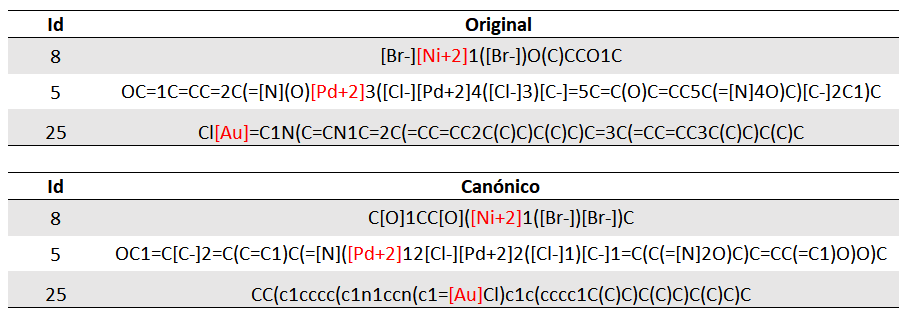
\includegraphics[scale=0.5]{imagenes/diseno/canonizado/canonicos_mal_implementacion.png}
    \caption{SMILES canónicos pertenecientes a la organometálica según el algoritmo propio de OpenBabel. Los metales están marcados en rojo. Son 3 moléculas del dataset mostrado en el Apéndice \ref{apend:pagina_tabla_intro_grande}, identificadas por su Id.} 
    \label{fig:canonicos_mal_implementacion}
\end{figure}



\subsubsection{Reglas canonizado} \label{reglas_canonizado}

Se busca por tanto, lo primero de todo colocar el metal al inicio del SMILES y en base a esto ir colocando el resto de átomos vecinos. Esto también se cree que sería beneficioso a la hora de trabajar con modelos generativos. El tener una estructura legible y estricta en donde se fije el metal al principio de la cadena favorece la robustez de la representación \cite{SELFIES, krenn_self_referencing_2020}.
En base a la premisa de colocar el metal lo primero, se ha desarrollado un sistema canónico con las siguientes reglas:
\begin{itemize}
    \item Tiene que haber un metal de interés para la organometálica (los metales de transición mencionados en la Sección \ref{teoria:ogm}) en el SMILES de entrada para aplicar el algoritmo de canonizado propio. En caso negativo, se aplicaría el original de OpenBabel. 
    \item Si el SMILES está desconectado (por fragmentos) se aplicará el algoritmo original. El SMILES resultado es la concatenación de cada fragmento canonizado por separado.
    \item Para escoger el metal que da inicio al SMILES se siguen las siguientes prioridades:
        \begin{enumerate}
            \item Si solamente hay un metal, se escoge dicho átomo directamente.
            \item Si hay más de 1 metal, se selecciona el que tiene mayor cantidad de subhijos (mayor tamaño de su subárbol) con respecto a los demás metales. Se considera que el metal más importante es del cuál dependen más átomos.
            \item Si la condición anterior resulta en empate, se toma el metal con mayor número atómico.
            \item Si la condición anterior resulta en empate, es decir, es el mismo elemento con la misma cantidad de subhijos, se toma el metal que de entre sus subhijos aparezcan menos carbonos. Ya que los carbonos son esenciales, son muy frecuentes. Por lo que se da prioridad a cualquier otro elemento antes.
            \item Si lo anterior también resulta en empate, todo indica que se trata de una molécula simétrica, por lo que no importa qué metal se escoja.
        \end{enumerate}
\end{itemize}

Se esboza a continuación un pseudo código en lenguaje natural que muestra el flujo de ejecución del método principal, \textit{CreateFragCanSmiStringOgm}, durante la canonización. 
\begin{algorithm}[h!]
   \caption{CreateFragCanSmiStringOgm}
   \If{no tiene metal $||$ está fragmentado}{aplicar algoritmo original}
   \textit{startAtom} $\longleftarrow$ Seleccionar el metal inicial \\
   \textit{canonicalLabels} $\longleftarrow$ Calcular los \textit{canonical labels}\\
   \textit{root} $\longleftarrow$ Generar el nodo raíz(starAtom)\\
   BuildCanonTree(\textit{root}, \textit{canonicalLabels})\\
   RearrangeTree(\textit{root})\\
   IdentifyBranches(\textit{root})\\
   ToCansmilesString(\textit{root}, \textit{buffer}, \textit{canonicalLabels})\\
   \textit{delete root} \\
   \label{tab:CreateFragCanSmiStringOgm}
\end{algorithm}

Mencionar del código anterior el método \textit{RearrangeTree}. Una vez se monta el árbol a través del método \textit{BuildCanonTree} usando el orden canónico calculado por OpenBabel, se realiza un post-procesado a dicho árbol para reordenar cada uno de los hijos en función de la longitud de sus subárboles, de menor a mayor. Esto se ejemplifica con la Figura \ref{fig:rearrangeTree}. Partimos del SMILES

\begin{center}
\small
\textit{O\#C[Fe+2]1234([I-])(C\#O)[CH]=5[CH]4=[CH]3[CH-]2[CH]51}    
\end{center}

que contiene un átomo de hierro central y 4 ramas: dos enlaces CO, un yodo, y un Cp. El primer árbol que se genera es el de la imagen izquierda, en donde las ramas hijas parecen no seguir ningún orden. El árbol de la derecha es el resultado de reordenar los hijos, colocando las ramificaciones de menor tamaño las primeras. De esta manera cuando el método \textit{ToCansmilesString} recorra el árbol para generar el SMILES canónico,  aparecerán antes. Podríamos decir que \textit{BuildCanonTree} se encarga de colocar los nodos verticalmente, asegurando una correcta relación padre-hijo entre los átomos; mientras que \textit{RearrangeTree} los ordena horizontalmente.

\begin{figure}[h!]
    \centering
    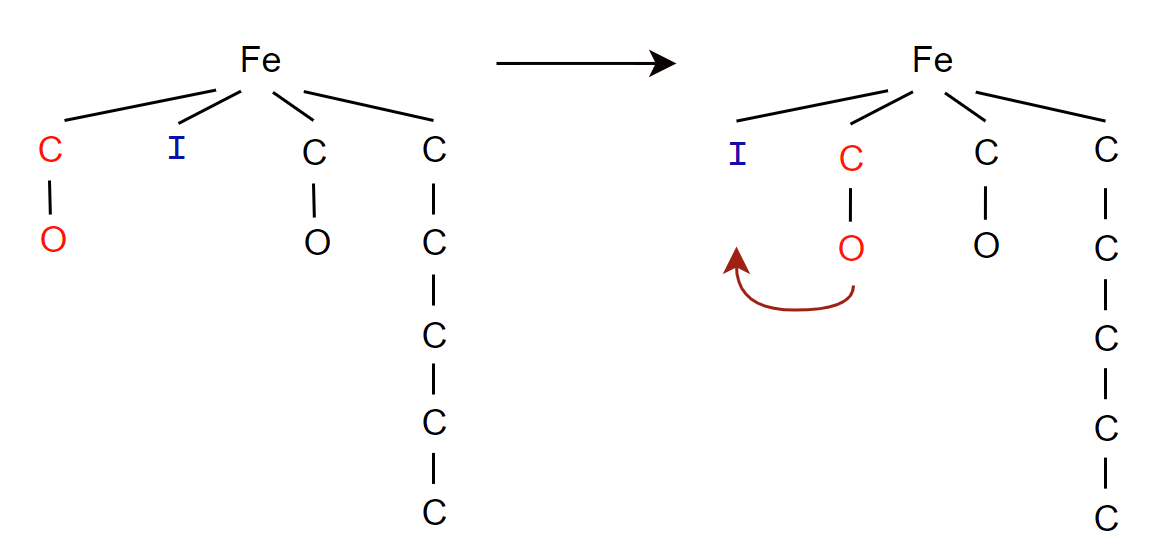
\includegraphics[scale=0.4]{imagenes/diseno/canonizado/rearrange.png}
    \caption{Reordenación de los hijos en función de la longitud de sus ramas. Imagen de elaboración propia. Molécula 28 del Apéndice \ref{apend:pagina_tabla_intro_grande}.}
    \label{fig:rearrangeTree}
\end{figure}

En la Figura \ref{fig:desempate_metales1} se muestra el caso para el SMILES 

\begin{center}
\textit{[Cl-][Au+][P](C=1C=CC=CC1)(C=2C=CC=CC2) [C-]34[CH]5=[CH]6[CH]7=[CH]3 [Fe+2]6789\%10\%1154[CH]=\%12[CH]\%11=[CH]\%10 [C-]9([CH]\%128)[P](C)C}
    
\end{center}

el cual tiene 2 metales: un átomo de hierro (Fe) y un átomo de oro (Au). Vemos los 2 árboles generados durante el proceso de selección: en el de la izquierda el hierro se coloca como nodo raíz y se evalúa el subárbol del oro, obteniendo 2 nodos (marcados en rojo); en el de la derecha el oro se coloca como nodo raíz y se evalúa el subárbol del hierro, obteniendo 22 nodos. Se escogerá por tanto el hierro como nodo raíz al tener más nodos que dependen de él. Notar que estos no son los árboles canónicos finales, sino árboles auxiliares cuyo único propósito es seleccionar el primer átomo. Observar también que a ninguno de los dos árboles se le ha aplicado el reordenamiento comentado antes.


\begin{figure}[h!]
\centering
\begin{subfigure}{.5\textwidth}
  \centering
  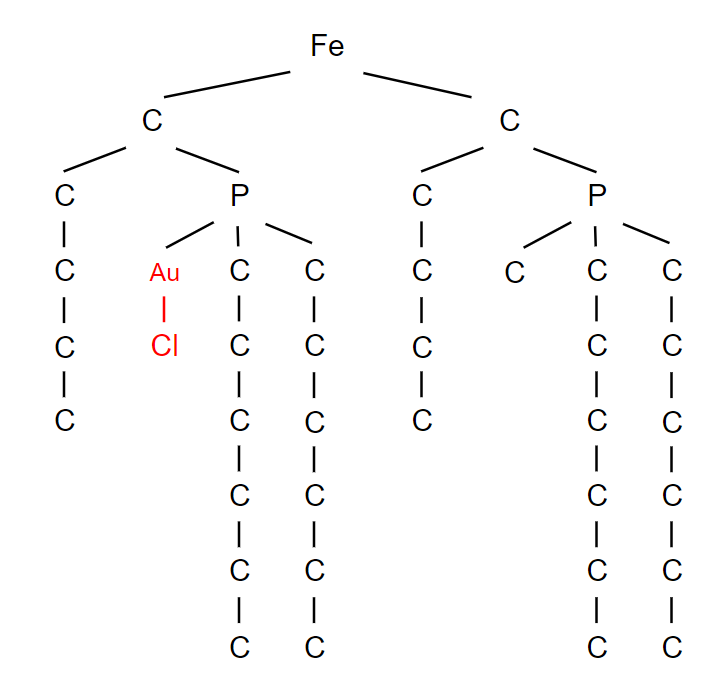
\includegraphics[width=.95\linewidth]{imagenes/diseno/canonizado/mol23Modified_Fe_raiz_resalte.png}
  \caption{}
\end{subfigure}%
\begin{subfigure}{.5\textwidth}
  \centering
  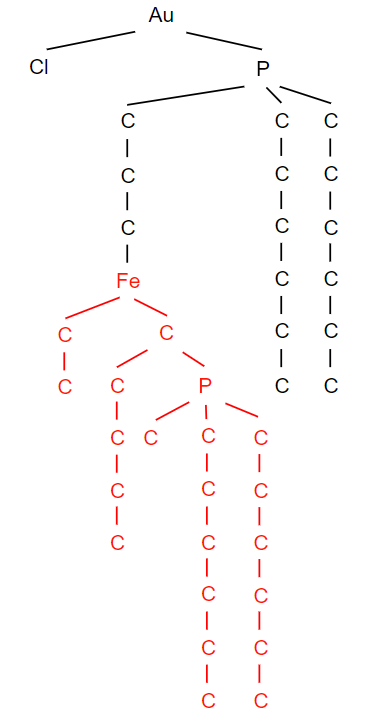
\includegraphics[width=.45\linewidth]{imagenes/diseno/canonizado/mol23Modified_Au_raiz_resalte.png}
  \caption{}
\end{subfigure}
\caption{Esquemas de los árboles generados para la selección del metal. Imagen de elaboración propia. \textbf{(a)} árbol con el hierro como raíz, el subárbol del oro solamente tiene 2 nodos; \textbf{(b)} árbol con el oro como raíz, el subárbol del hierro tiene 22 nodos. Imagen de elaboración propia.}
\label{fig:desempate_metales1}
\end{figure}



\subsection{Sistema de representación 2D} \label{implementacion:dibujado}

Al generar representaciones 2D de una molécula pueden surgir muchas dificultades relacionadas con la disposición de los átomos como su orientación o intentar evitar el solapamiento; y relacionadas con el texto, tipo y tamaño de letra, uso o no de abreviaturas, alineación y posición relativa de las etiquetas con respecto a los demás átomos, etc. Estos problemas se pueden superan de mejor o peor manera mediante una serie de algoritmos, pero por ahora, ninguno es tan versátil como para ajustarse a cualquier tipo de estructura química \cite{david_molecular_2020}. Para más detalles y ejemplos de algoritmos de representación 2D y sus limitaciones en diferentes toolkits (RDKit, OpenBabel, CDK, Avalon e Indigo), se recomienda ver la presentación de 2016 de John Mayfield \cite{comparative_depictions}.

En lo que respecta a este proyecto, se han llevado a cabo 2 modificaciones en el sistema de visualización de OpenBabel para representar moléculas:
\begin{enumerate}
    \item Se ha aumentado la longitud de los enlaces entre átomos para una mayor claridad y separación. Para moléculas organometálicas, en donde un mismo átomo normalmente tiene varios enlaces y existen muchos ciclos, el mero hecho de espaciar un poco los enlaces ya ayuda a que no se vea todo tan solapado.
    \item Se han centrado los esfuerzos en la detección y mejora de visualización de estructuras tipo Cp, muy comunes en organometálica (ver Sección \ref{teoria:ogm}).
\end{enumerate}


Para el segundo punto, se han visualizado una gran cantidad de moléculas que contienen Cp para averiguar las maneras más frecuentes en las que se suelen describir y visualizar. Existen varias maneras de representar compuestos de coordinación con ligandos Cp usando enlaces convencionales (Figura \ref{fig:ferrocene_options}), pero ninguna opción refleja correctamente las propiedades de este tipo de uniones.
\begin{figure}[h!]
    \centering
    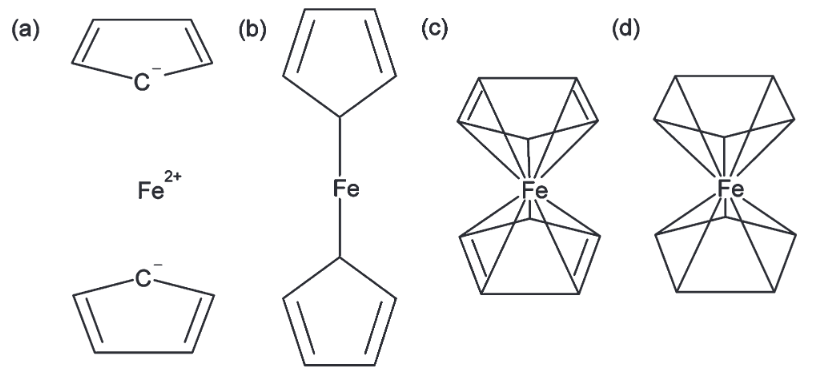
\includegraphics[scale=0.5]{imagenes/diseno/dibujo/varios_intentos_ferroceno.png}
    \caption{Intentos para representar el ferroceno usando enlaces convencionales. \textbf{(a)} ni si quiera representa los enlaces, dibujando varios fragmentos desconectados; \textbf{(b)} mantiene intactos los recuentos de valencia orgánica, desconectando los carbono de enlaces dobles; \textbf{(c)} Ignora las restricciones de valencia normales e incluye todos los enlaces átomo-átomo posibles; \textbf{(d)} representa todos los enlaces significativos a costa de los dobles enlaces. Imagen y descripción extraída y traducida de \cite{zero_order}.}
    \label{fig:ferrocene_options}
\end{figure}

Se han valorado otras opciones ya existentes en la literatura, como lo que propone Alex M. Clark en la publicación \textit{``Accurate Specification of Molecular Structures: The Case for Zero-Order Bonds and Explicit Hydrogen Counting"} \cite{zero_order}. Se puede ver en la Figura \ref{fig:zero_bond_ferrocene} el resultado de su propuesta usando lo que él llama enlaces de orden cero (zero-order bonds). 
\begin{figure}[h!]
    \centering
    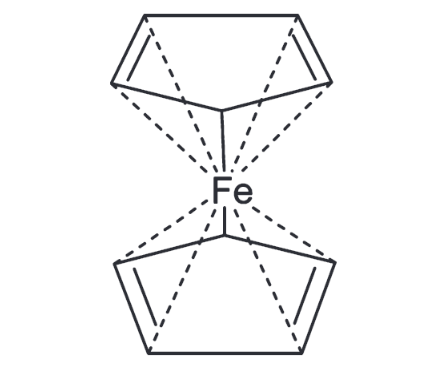
\includegraphics[scale=0.4]{imagenes/diseno/dibujo/zero_bond_orders_ferrocene.png}
    \caption{Ferroceno utilizando enlaces de orden cero según Alex M. Clark. Imagen extraída de \cite{zero_order}.}
    \label{fig:zero_bond_ferrocene}
\end{figure}

Aun así, no se diferencia mucho de la Figura \ref{fig:ferrocene_options}(c) y tampoco termina de ajustarse a cómo los químicos suelen representarlos. Se ha intentado seguir por tanto el manual de la IUPAC \textit{``Graphical representation standards for chemical structure diagrams (IUPAC Recommendations 2008)''} \cite{iupac_manual}, que alberga una gran cantidad de casuísticas con todos los aspectos relacionados a la representación gráfica de la estructura molecular, explicadas de manera detallada y rigurosa. Concretamente en las secciones GR-1.7.1 y GR-6 del manual hablan sobre los enlaces de coordinación, enlaces de ciclos aromáticos y electrones deslocalizados. Con lo anterior y atendiendo a las recomendaciones de los expertos, el objetivo es implementar la forma mostrada en la Figura \ref{fig:metalocenos_ejemplos}(a) ya que capta la aromaticidad y geometría de los enlaces del ligando.


A todo lo anterior se nos suma el concepto de percepción de anillos, una problemática para nada trivial y que ha estado siempre presente en en mundo de las chemoinformatics. Para entender esto, imaginemos que tenemos una molécula con un anillo de \textit{decalina} (10 carbonos). A la hora de identificar y almacenar la pertenencia a ciclos de cada uno de los átomos no podemos simplemente utilizar todas las combinaciones de ciclos existentes (Figura \ref{fig:decalina_all_ciclos}), ya que haría que un conjunto de átomos pertenezcan simultáneamente a varios anillos (en este caso los átomos 4 y 5). Ejemplo extraído de \cite{sssr_smallest_2020}. Esto según las necesidades de cada aplicación puede suponer un problema o no.

\begin{figure}[h!]
    \centering
    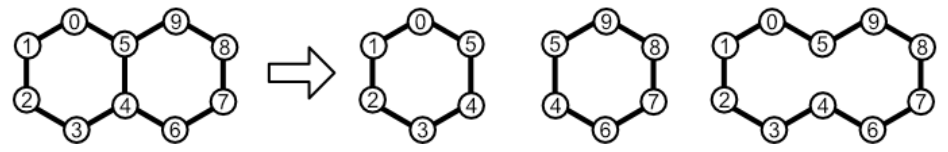
\includegraphics[scale=0.5]{imagenes/diseno/dibujo/decalina_all_cycles.png}
    \caption{Decalina y todo su subset de ciclos.}
    \label{fig:decalina_all_ciclos}
\end{figure}

Por lo general, los algoritmos en los toolkits de chemoinformatics requieren un set de ciclos filtrado, únicamente con los ciclos más pequeños y relevantes. Para el caso anterior, bastaría si nos quedáramos solamente con cualquier combinación de 2 de los 3 ciclos, teniendo así todo el espacio de ciclos cubierto. Esto se puede alcanzar con el algoritmo de SSSR (Smallest Set of Smallest Rings), siendo el que más se usa hoy día para la percepción de anillos \cite{sssr_smallest_2020, sssr_harmful,sssr_counterexamples_2004, sssr_review_1989}. 

La percepción SSSR es la que utiliza OpenBabel y por lo general funciona bien para cualquier tipo de molécula. Pero justamente a la hora de representar estructuras Cp, la forma en la que los átomos de carbono se unen con el metal hace que se genere un conjunto de ciclos que dificulta los algoritmos de detección. Se ilustra este problema con la Figura \ref{fig:sssr_iron(II)}. Supongamos que un hierro (Fe) se une con un ligando Cp. Vemos que cada par de carbonos forma un ciclo de tamaño 3 junto con el hierro, desapareciendo el ciclo original entre los propios carbonos, de manera que internamente tenemos los ciclos almacenados como ``3-1-2, 4-1-3, 5-1-6, 6-1-2 y 5-1-4". Por defecto OpenBabel trata los enlaces como en la Figura \ref{fig:ferrocene_options}(c) y teniendo en cuenta el tratamiento de los ciclos, en la mayoría de casos obtenemos resultados como los de la Figura \ref{fig:iron(II)Original}, ya que a la hora de colocar las líneas de los enlaces, los toma como anillos independientes.

\begin{figure}[h!]
    \centering
    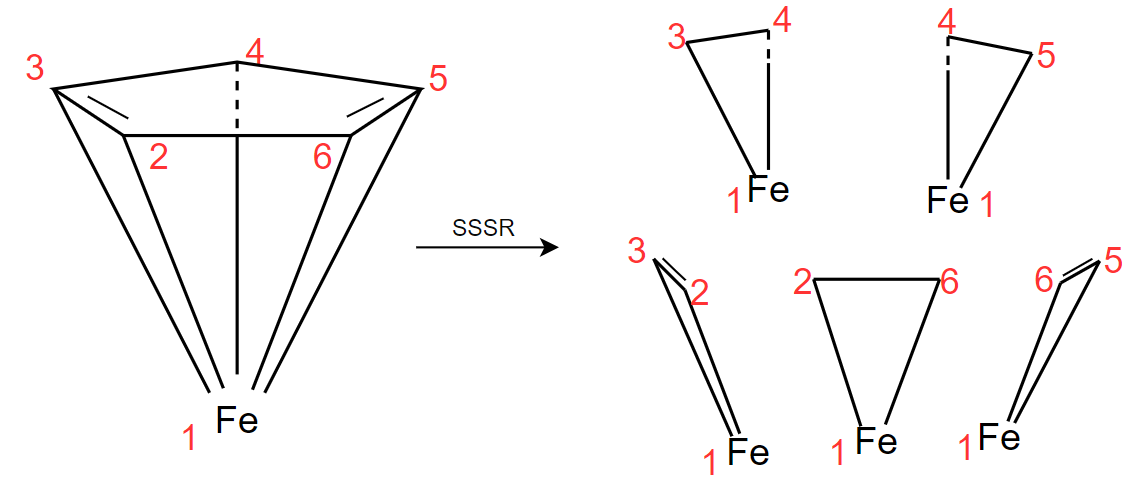
\includegraphics[scale=0.35]{imagenes/diseno/dibujo/sssr_iron.png}
    \caption{Conjunto de ciclos según la percepción SSSR para un hierro con un ligando Cp. Imagen de elaboración propia.}
    \label{fig:sssr_iron(II)}
\end{figure}


\begin{figure}[h!]
    \centering
    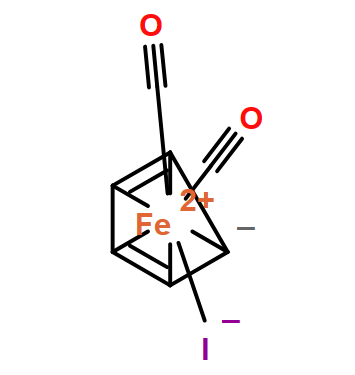
\includegraphics[scale=0.5]{imagenes/diseno/dibujo/iron(II)_Original.png}
    \caption{Representación 2D de la molécula \textit{Dicarbonylcyclopentadienyliodoiron(II)} generada con OpenBabel. Molécula 28 del Apéndice \ref{apend:pagina_tabla_intro_grande}.}
    \label{fig:iron(II)Original}
\end{figure}

\subsubsection{Reglas de detección} \label{reglas_deteccion_cp}

Además, hay que tener en cuenta otras situaciones a la hora de detectar Cps completos. Si en la misma molécula hay más de un Cp, cómo se detectan y diferencian cada uno de las estructuras o cómo sabemos qué carbonos forman parte de un Cp o de otro. A través de la cadena SMILES no se puede obtener esa información ya que todos los enlaces son iguales (un metal con un carbono) y la percepción SSSR complicaba más aun la identificación de pertenencia de los carbonos al mismo anillo. En base a esto, surge la identificación por bloques. Se utiliza para esto el árbol canónico explicado previamente con el objetivo identificar relaciones padre-hijo o relaciones de dependencia entre átomos, indicando la pertenencia a una misma subestructura, en este caso a un mismo Cp.

Por tanto, las reglas de detección para una estructura Cp se pueden resumir en:
\begin{itemize}
    \item Que exista un enlace Metal-Carbono (M-C)
    \item Que el carbono pertenezca a un bloque y que los demás carbonos del mismo bloque tengan también un enlace M-C con el mismo metal que el resto del bloque.
\end{itemize}

Una vez se identifiquen correctamente, se activa un flag especial para marcar qué átomos pertenecen o no a un Cp y darles un tratamiento distinto a la hora de dibujarlos. En concreto:  
\begin{enumerate}
    \item Se crea un único átomo nuevo a modo de señuelo (átomo especial en OpenBabel con número atómico 0, \textit{dummy}) para que enlace con el metal.
    \item En base a ese nuevo átomo dummy, se modifican las coordenadas 2D de los carbonos de interés y se disponen en forma de polígono.
    \item Se calcula el círculo central mediante una serie de coordenadas y tanto al círculo como al polígono se le da una perspectiva rotándolos sobre el eje X.
    \item Finalmente se eliminan todos los enlaces M-C para que OpenBabel no los dibuje automáticamente. El hecho de eliminar los enlaces no supone ningún problema ya que no se realizan más operaciones a posteriori que puedan necesitarlos.
\end{enumerate} 

Todo lo relacionado con cada Cp individual se almacena en la clase CpComplex, guardando información como la lista de carbonos que forman el Cp, el metal al que están asociados, el átomo dummy que lo posiciona y el centroide del polígono entre otras cosas.

En el siguiente capítulo se muestran los resultados alcanzados tras la implementación.
















\chapter{Resultados y pruebas}

En las siguientes secciones se expondrán los resultados que se han obtenido tras usar la nueva nomenclatura implementada y los cambios en el sistema de representación. Se describirán también las pruebas llevadas a cabo para validar todo este proceso.

\section{Nomenclatura canónica}

Para la canonización, se muestra en la siguiente Tabla \ref{tab:canon_smiles} una comparativa entre el SMILES original, el SMILES canónico obtenido utilizando únicamente el algoritmo de OpenBabel (\textit{canonicalLabels}), y el SMILES canónico obtenido utilizando el algoritmo implementado. Se agrupan en bloques de 3, siendo cada línea con separación cada uno de los SMILES en el orden comentado. No aparecen todas las moléculas del dataset en la tabla ya que se haría excesivamente grande; se han introducido algunas de manera aleatoria para ver los cambios entre las nomenclaturas. Las demás estarán disponibles para su consulta en GitHub en la carpeta \textit{`output/smiles'}.

\begin{longtable}{m{0.3cm}>{\arraybackslash}m{11.5cm}}
\caption{Se muestran los SMILES en este orden: original, openbabel, implementación propia. Los Id hacen referencia al Anexo \ref{apend:pagina_tabla_intro_grande}.}\\
\toprule
 \textbf{Id} & \textbf{SMILES} \\ \midrule
\endfirsthead

\multicolumn{2}{c}%
{{\bfseries \tablename\ \thetable{} -- Continuación de la página anterior}} \\
\toprule
\textbf{Id} & \textbf{SMILES} \\ \midrule
\endhead

\hline \multicolumn{2}{r}{{Continúa en la siguiente página}} \\
\endfoot

\hline
\endlastfoot

% Mol 3
 % \multirow{3}{*}{3} & %$\rightarrow$ &
 & [Cl-][Pd+2]123([Cl-])[CH]=4CC[CH]3=[CH]2CC[CH]41      \\ [0.3cm]
 3 & [Cl-][Pd+2]123([Cl-])[CH]4=[CH]3CC[CH]2=[CH]1CC4               \\ [0.3cm]
 & [Pd+2]123([Cl-])([Cl-])[CH]4=[CH]3CC[CH]1=[CH]2CC4               \\ 
\midrule

% Mol 4
 % \multirow{3}{*}{4} & %$\rightarrow$ &
 & [Cl-][Pd+2]1([C-]=2C=CC=CC2C=3C=CC=CC3[N]1(C)C)[PH](C4C C5CCC4C5)C6CC7CCC6C7      \\ [0.5cm]
 4 & [Cl-][Pd+2]1([C-]2=C(C=CC=C2)c2ccccc2[N]1(C)C)[PH](C1C C2CCC1C2)C1CC2CCC1C2               \\ [0.5cm]
 & [Pd+2]1([Cl-])([PH](C2CC3CC2CC3)C2CC3CC2CC3)[C$-$]2=C(C= CC=C2)c2c([N]1(C)C)cccc2              \\ 
\midrule

% Mol 5
 % \multirow{3}{*}{5} & %$\rightarrow$ &
 & OC=1C=CC=2C(=[N](O)[Pd+2]3([Cl-][Pd+2]4([Cl-]3)[C-]=5C=C (O)C=CC5C(=[N]4O)C)[C-]2C1)C      \\ [0.7cm]
 5 & OC1=C[C-]2=C(C=C1)C(=[N](O)[Pd+2]12[Cl$-$][Pd+2]2([Cl$-$]1)[C$-$] 1=C(C=CC(=C1)O)C(=[N]2O)C)C               \\ [0.7cm]
 & [Pd+2]12([C-]3=C(C(C)=[N]2O)C=CC(O)=C3)[Cl$-$][Pd+2]2([Cl$-$]1) [C$-$]1=C(C(C)=[N]2O)C=CC(O)=C1               \\ 
\midrule



% Mol 7
 % \multirow{3}{*}{7} & %$\rightarrow$ &
 & O=S(=O)([NH-][Pd+4]12([F-])([C-]=3C=CC=CC3C(C)(C)[CH2$-$]1) [N]=4C=CC=CC4C=5C=CC=C[N]52)C6=CC=C(C=C6)C      \\ [0.7cm]
 7 & O=S(=O)([NH-][Pd+4]12([F-])([C-]3=C(C=CC=C3)C(C)(C)[CH2$-$]1) [N]1=C(C=CC=C1)C1=[N]2C=CC=C1)c1ccc(cc1)C               \\ [0.7cm]
 & [Pd+4]12([F-])([CH2-]C(C)(C)C3=[C-]2C=CC=C3)([NH-]S(=O)(=O)c2 ccc(C)cc2)[N]2=C(C=CC=C2)C2=[N]1C=CC=C2               \\ 
\midrule



% Mol 15
 % \multirow{3}{*}{15} & %$\rightarrow$ &
 & [Cl-][Au+][P](C=1C=CC=CC1C=2C=CC=CC2)(C(C)(C)C)C(C)(C)C      \\ [0.5cm]
 15 & [Cl-][Au+][P](c1ccccc1c1ccccc1)(C(C)(C)C)C(C)(C)C               \\ [0.5cm]
 & [Au+]([Cl-])[P](C(C)(C)C)(C(C)(C)C)c1ccccc1c1ccccc1               \\ 
\midrule


% Mol 18
 % \multirow{3}{*}{18} & %$\rightarrow$ &
 & [Cl-][Au+][P](C=1C=CC=CC1C=2C(=CC(=CC2C(C)C)C(C)C)C(C) C)(C3CCCCC3)C4CCCCC4      \\ [0.5cm]
 18 & [Cl-][Au+][P](c1ccccc1c1c(cc(cc1C(C)C)C(C)C)C(C)C)(C1CCCC C1)C1CCCCC1               \\ [0.5cm]
 & [Au+]([Cl-])[P](C1CCCCC1)(C1CCCCC1)c1ccccc1c1c(C(C)C)cc(C (C)C)cc1C(C)C               \\ 
\midrule

% Mol 19
 % \multirow{3}{*}{19} & %$\rightarrow$ &
 & [Cl-][Au+][P](C=1C=CC=CC1C2=C(OC(C)C)C=CC=C2OC(C)C) (C=3C=CC=CC3C4=C(OC(C)C)C=CC=C4OC(C)C)C5CCCCC5     \\ [0.7cm]
 19 & [Cl-][Au+][P](c1ccccc1c1c(OC(C)C)cccc1OC(C)C)(c1c cccc1c1c(OC(C)C)cccc1OC(C)C)C1CCCCC1               \\ [0.7cm]
 & [Au+]([Cl-])[P](C1CCCCC1)(c1ccccc1c1c(OC(C)C)ccc c1OC(C)C)c1ccccc1c1c(OC(C)C)cccc1OC(C)C               \\ 
\midrule



% Mol 24
 % \multirow{3}{*}{24} & %$\rightarrow$ &
 & Cl[Au]=C1N(C=CN1C=2C(=CC(=CC2C)C)C)C=3C(=CC(=CC3C)C)C      \\ [0.3cm]
 24 & Cl[Au]=c1n(ccn1c1c(cc(cc1C)C)C)c1c(cc(cc1C)C)C               \\ [0.3cm]
 & [Au](Cl)=c1n(c2c(C)cc(C)cc2C)ccn1c1c(C)cc(C)cc1C               \\ 
\midrule


% Mol 28
 % \multirow{3}{*}{28} & %$\rightarrow$ &
 & O\#C[Fe+2]1234([I-])(C\#O)[CH]=5[CH]4=[CH]3[CH-]2[CH]51      \\ [0.3cm]
 28& [O]\#C[Fe+2]1234([I-])(C\#[O])[CH]5=[CH]4[CH-]3[CH]2=[CH]15               \\ [0.3cm]
 & [Fe+2]1234([I-])(C\#[O])(C\#[O])[CH-]5[CH]3=[CH]2[CH]1=[CH]45         \\      
\midrule

% Mol 30
 % \multirow{3}{*}{30} & %$\rightarrow$ &
 & [I-][Ir+3]12345([I-][Ir+3]6789([I-])([I-]1)C=\%10(C)C9(C)=C8(C)[C$-$] 7(C)C\%106C)C=\%11(C)C5(C)=C4(C)[C-]3(C)C\%112C      \\ [0.7cm]
 30 & [I-][Ir+3]12345([I-][Ir+3]6789([I-])([I-]1)[C]1(=[C]9([C$-$]8([C]7(=[C]61 C)C)C)C)C)[C]1(=[C]5([C-]4([C]3(=[C]21C)C)C)C)C               \\ [0.7cm]
 & [Ir+3]12345([I-])([C-]6(C)[C]1(C)=[C]3(C)[C]4(C)=[C]26C)[I$-$] [Ir+3]1234([I-]5)([I-])[C]5(C)=[C]3(C)[C]2(C)=[C]1(C)[C-]45C               
% \midrule

\label{tab:canon_smiles}
\end{longtable}

\pagebreak

Con esta solución en donde se organiza el SMILES según sus ramificaciones, se ha intentado también dar un enfoque al canonizado orientado a la representación 2D. De esta manera, podemos visualizar ambos e identificar claramente la correspondencia entre una porción contigua del SMILES con una sección de la representación gráfica. Así, se recorren primero todos los vecinos con menor longitud de un átomo hasta cerrar esa rama antes de pasar a la siguiente, obteniendo un SMILES más limpio y evitando que átomos individuales se queden al final de ramificaciones muy largas. Esto se puede ver en la Figura \ref{fig:smiles_vs_dibujo}.

\begin{figure}[h!]
\begin{subfigure}{.9\textwidth}
  \centering
  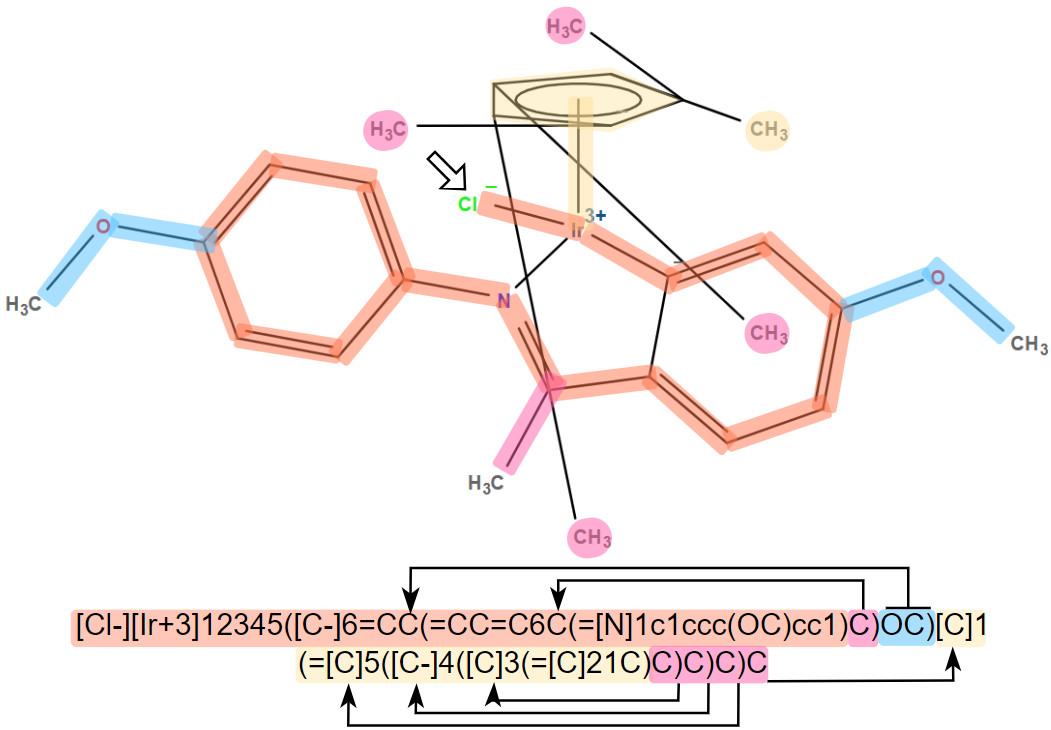
\includegraphics[width=.8\linewidth]{imagenes/resultados/moleculas/mol31_subrayao_malCanon.png}
  \caption{Canónico de OpenBabel}
\end{subfigure}%
\\
\\
\begin{subfigure}{.9\textwidth}
  \centering
  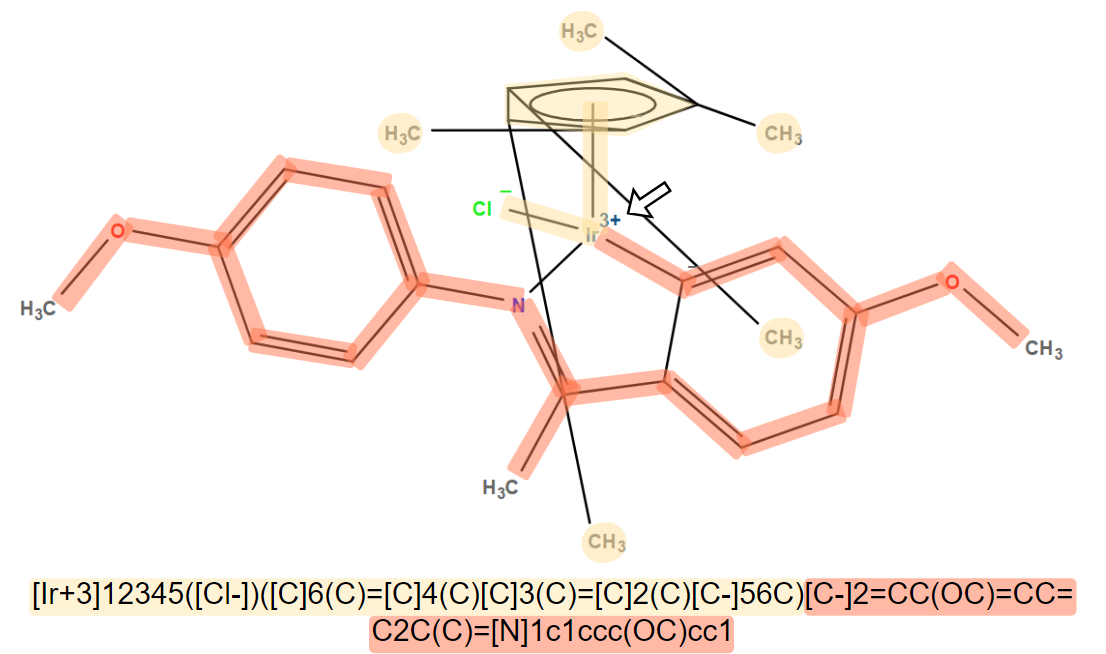
\includegraphics[width=.8\linewidth]{imagenes/resultados/moleculas/mol31_subrayao.png}
  \caption{Canónico propio}
\end{subfigure}
\caption{Correspondencia entre el SMILES canónico y la representación 2D de la molécula . \textbf{(a)} representación 2D usando solamente el algoritmo de OpenBabel; y \textbf{(b)} usando mi algoritmo de selección de metales y reordenación de ramas. La flecha indica el inicio del SMILES. Imagen de elaboración propia.}
\label{fig:smiles_vs_dibujo}
\end{figure}

\newpage

\section{Respresentación 2D}
Con respecto al cambio en la longitud de los enlaces, si bien no arregla el solapamiento de moléculas complejas, ya que esto requeriría de un cambio sustancial en el algoritmo de generación de coordenadas (si no, un rediseño completo), mejora en cierta medida la visibilidad de los enlaces. La diferencia es sutil, y las líneas tienen un trazado más fino. Pero para moléculas de este tipo donde todo aparece muy solapado y según las recomendaciones de los expertos, son preferibles estos resultados y que salga todo un poco más espaciado. En la Figura \ref{fig:bonds_longitud} se muestran los resultados para un par de moléculas del dataset.

\begin{figure}[h]
    \centering
    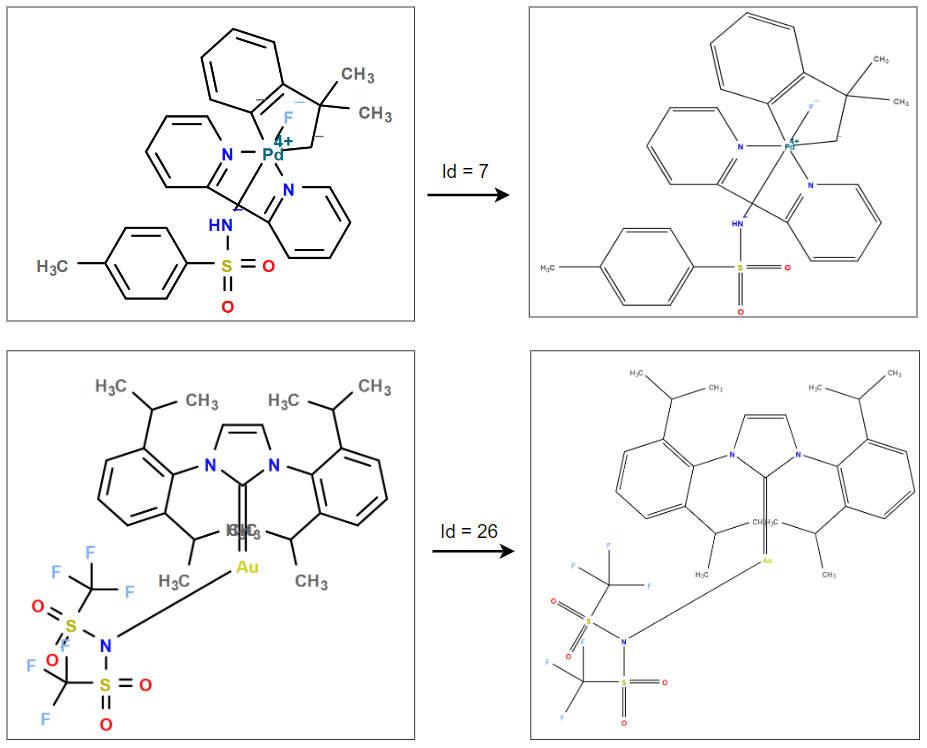
\includegraphics[scale=0.51]{imagenes/resultados/bond_longitud.png}
    \caption{Comparativa en la representación según la longitud de sus enlaces. A la izquierda las moléculas originales; a la derecha las moléculas con la longitud de enlaces aumentada.}
    \label{fig:bonds_longitud}
\end{figure}


En cuanto a la representación 2D de los Cp, se presenta en la Figura \ref{fig:evolucion_iron} la evolución en el proceso de dibujado mediante capturas intermedias. Según lo discutido en la Sección \ref{implementacion:dibujado}, finalmente obtenemos el resultado buscado con la Figura \ref{fig:evolucion_iron_d}. En la Tabla \ref{tab:cps_dibujado} se muestran los resultados para las moléculas con estructuras Cp en nuestro dataset. Podemos apreciar una mejora considerable en la representación, notando como todo el ligando Cp se detecta y transforma.

Aquellas moléculas cuya representación no varía no se incluyen en este documento. Los ficheros `.svg' completos con todas las moléculas del dataset con el antes y el después están disponibles para su consulta en GitHub (en la carpeta `\textit{output/depictions}'), por lo que se podrán inspeccionar y hacer zoom de manera detallada. Por su parte, los expertos han proporcionado las representaciones que ellos mismos harían a mano para algunas de las moléculas del dataset. En el Anexo \ref{apend:expertos_dibujos} se puede ver una comparativa entre los dibujos de los expertos, los resultados obtenidos y los de ambas bases de datos.

\begin{figure}[h]
\centering
\begin{subfigure}{.35\textwidth}
  \centering
  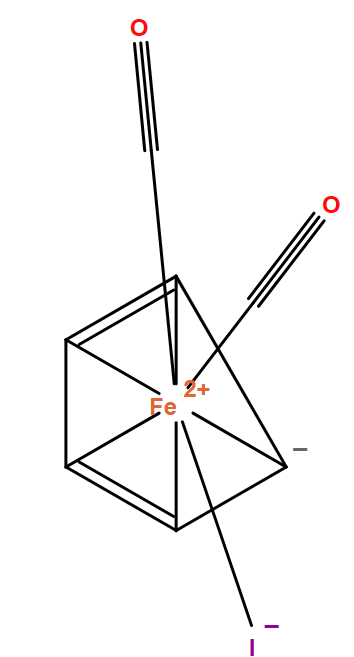
\includegraphics[width=.45\linewidth]{imagenes/resultados/evolucion_iron_a.png}
  \caption{}
\end{subfigure}%
\begin{subfigure}{.35\textwidth}
  \centering
  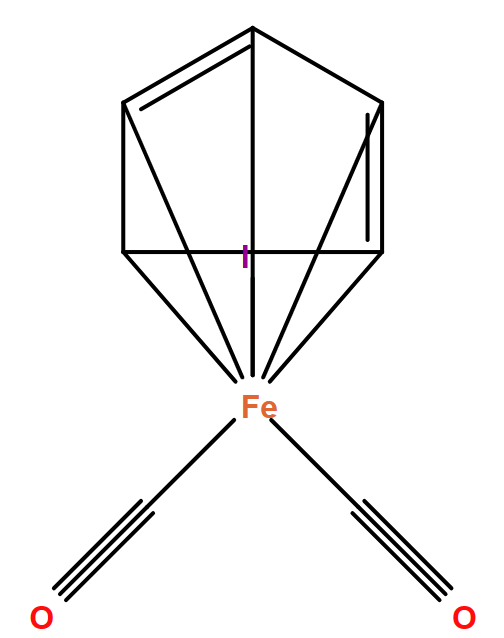
\includegraphics[width=.6\linewidth]{imagenes/resultados/evolucion_iron_b.png}
  \caption{}
\end{subfigure}%
\\
\begin{subfigure}{.35\textwidth}
  \centering
  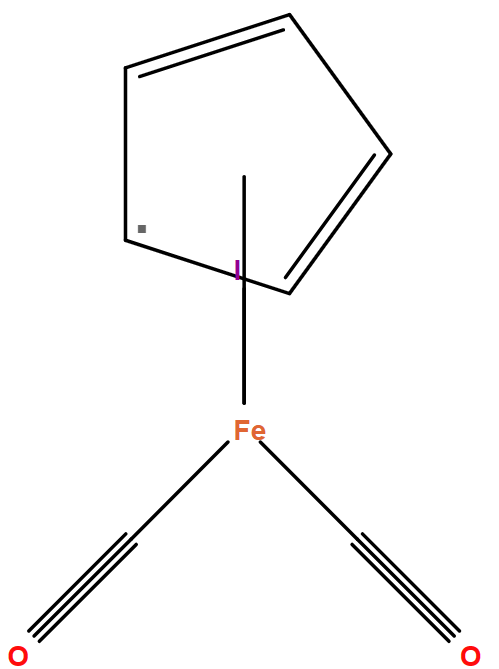
\includegraphics[width=.55\linewidth]{imagenes/resultados/evolucion_iron_c.png}
  \caption{}
\end{subfigure}%
\begin{subfigure}{.35\textwidth}
  \centering
  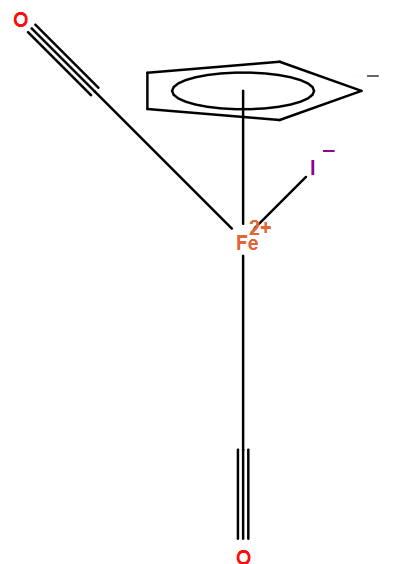
\includegraphics[width=.5\linewidth]{imagenes/resultados/moleculas/iron(II).png}
  \caption{}
  \label{fig:evolucion_iron_d}
\end{subfigure}%
\caption{Evolución durante la implementación del sistema de representación. Se muestra la molécula \textit{Dicarbonylcyclopentadienyliodoiron(II)} con Id 28 en el Anexo \ref{apend:pagina_tabla_intro_grande}. \textbf{(a)} original; \textbf{(b)} detección del Cp y modificación de la posición de los carbonos; \textbf{(c)} eliminación de enlaces y formación del polígono; y \textbf{(d)} polígono con perspectiva y curva central.}
\label{fig:evolucion_iron}
\end{figure}


% \newpage

\begin{longtable}{c>{\centering}m{5cm}>{\centering\arraybackslash}m{5.9cm}}
\caption{Resultados finales de los cambios en la representación para moléculas con Cp. Los Id hacen referencia al Anexo \ref{apend:pagina_tabla_intro_grande}.}\\

\toprule
 \textbf{Id} & \textbf{Original} & \textbf{Resultado} \\ \midrule
\endfirsthead

\multicolumn{3}{c}%
{{\bfseries \tablename\ \thetable{} -- Continuación de la página anterior}} \\
\toprule
\textbf{Id} & \textbf{Original} & \textbf{Resultado} \\ \midrule
\endhead

\hline \multicolumn{3}{r}{{Continúa en la siguiente página}} \\
\endfoot

\hline
\endlastfoot

% Mol 23
 23 & 
 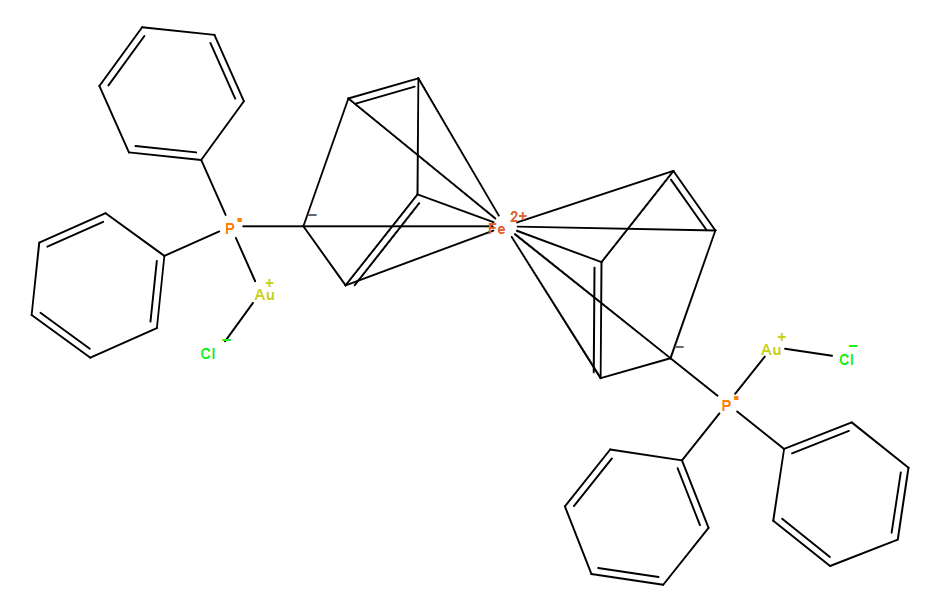
\includegraphics[width=4.3cm]{imagenes/resultados/cps/mol23_original.png} & 
 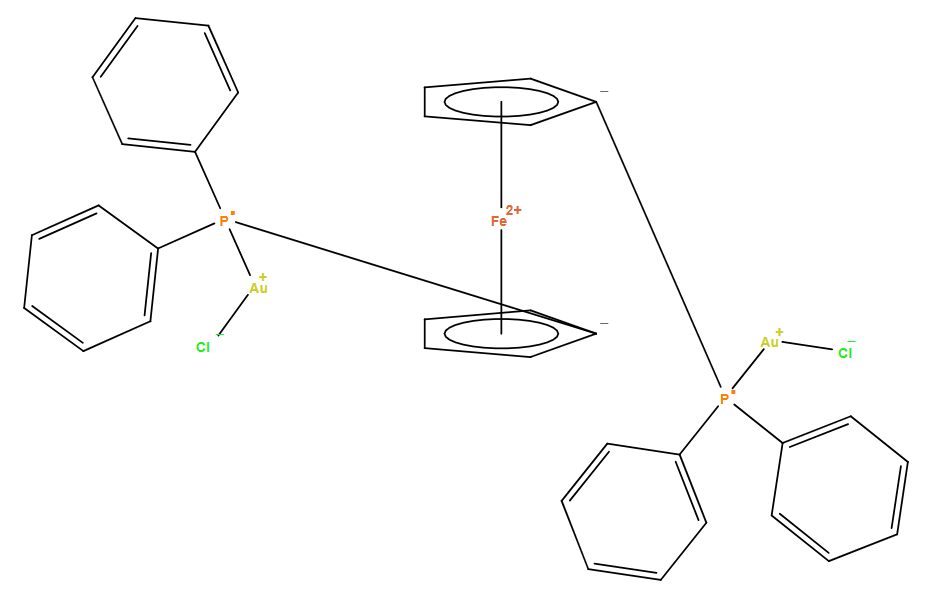
\includegraphics[width=4.3cm]{imagenes/resultados/cps/mol23_cp.png} \\
\midrule

% Mol 27
 27 &
 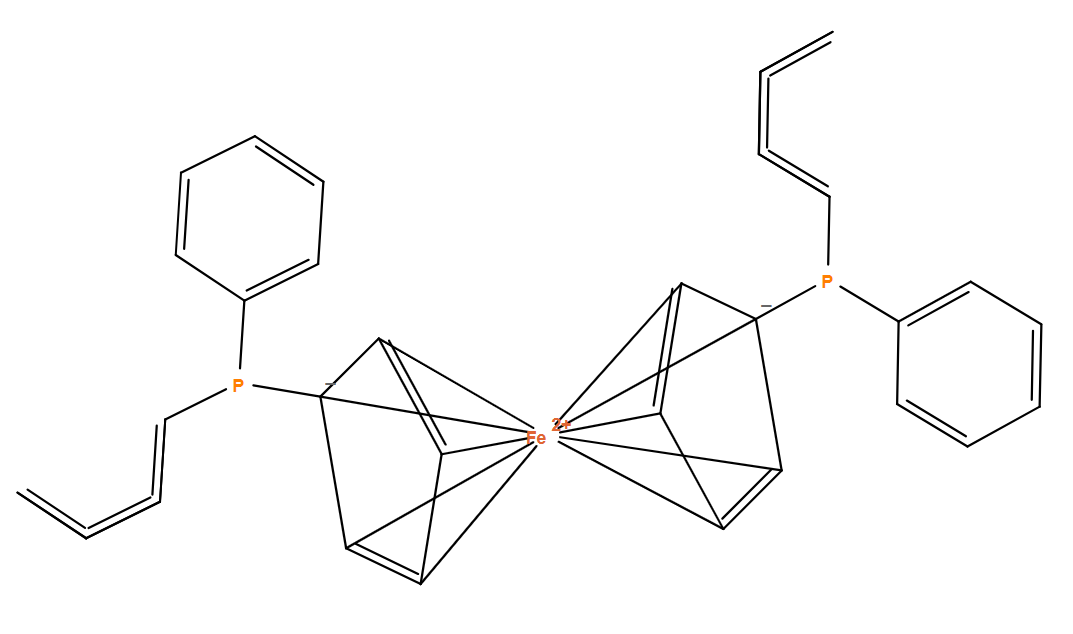
\includegraphics[width=4.3cm]{imagenes/resultados/cps/mol27_original.png} & 
 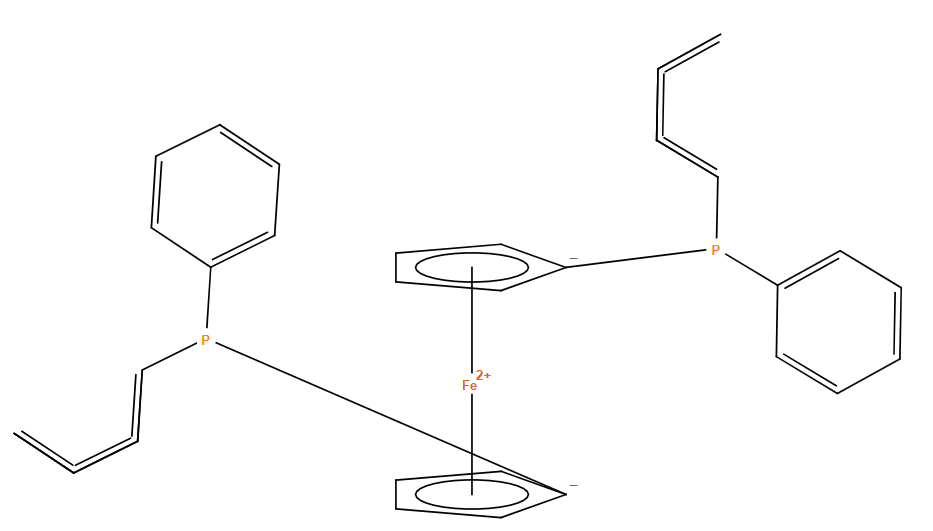
\includegraphics[width=4.3cm]{imagenes/resultados/cps/mol27_cp.png} \\
\midrule

% Mol 28
 28 &
 \includegraphics[width=2.5cm]{imagenes/resultados/cps/iron(II)_original.png} & 
 \includegraphics[width=2.5cm]{imagenes/resultados/moleculas/iron(II).png} \\
\midrule

% Mol 30
 30 &
 \includegraphics[width=4.3cm]{imagenes/resultados/cps/mol30_original.png} & 
 \includegraphics[width=4.3cm]{imagenes/resultados/cps/mol30_cp.png} \\
\midrule

% Mol 31
 31 &
 \includegraphics[width=4.3cm]{imagenes/resultados/cps/mol31_original.png} & 
 \includegraphics[width=4.3cm]{imagenes/resultados/cps/mol31_cp.png} 
% \midrule

\label{tab:cps_dibujado}
\end{longtable}




\subsection{Estructuras similares}
Destacar que la detección de estructuras Cp funciona de tal manera que no se limita estrictamente a enlaces de ligandos $\eta^{5}$-$C_{5}H_{5}$. Se es capaz de representar con el mismo estilo de dibujado ligandos de tipo $\eta^{x}$-$C_{x}H_{y}$, donde $[x \geq 3; 0 \leq y \leq x]$. Lo apreciamos en la siguiente Figura \ref{fig:n6_ligand_cp} con una estructura $\eta^{6}$-$C_{6}H_{4}$.

\begin{figure}[h!]
    \centering
    \includegraphics[scale=0.32]{imagenes/resultados/moleculas/Rutenio_n6_ligand_vs_original.png}
    \caption{Rutenio enlazado a un ligando `$\eta^{6}$-p-cyeme' junto con su cadena SMILES. Es una estructura que puede formar parte por ejemplo de moléculas experimentales bioactivas anti-cáncer \cite{rutenio_diimines_2018}.}
    \label{fig:n6_ligand_cp}
\end{figure}




% \newpage

\subsection{Alias o abreviaciones}
Finalmente, comentar una de las opciones de representación gráfica que tiene disponible OpenBabel. Se trata de la generación de alias o abreviaturas. Esto consiste en sustituir una estructura completa por una etiqueta en texto con su nombre abreviado. Se utiliza para ello un fichero de datos que contiene un conjunto de abreviaciones estándar conocidas junto con su cadena SMILES equivalente. OpenBabel almacena estos datos en `\textit{/openbabel-3.1.1/data/superatom.txt}', de manera que modificando dicho fichero se pueden incluir estructuras de interés para su abreviación.

De este modo se ahorra un poco de espacio en las representaciones gráficas y se favorece su legibilidad evitando algunos casos de solapamientos, sobre todo causados por ciclos de benceno que son los que más lugar ocupan. Esta funcionalidad se invoca con los parámetros por línea de órdenes `\textit{$--$genalias $-$xA}'. Se muestran algunas comparaciones, de las versiones sin alias y con alias en la Tabla \ref{tab:alias_vs_no_alias}.


\begin{longtable}{c>{\centering}m{5cm}>{\centering\arraybackslash}m{5.9cm}}
\caption{Comparativa de algunas representaciones 2D entre su versión normal y su alternativa usando abreviaciones. Los Id hacen referencia al Anexo \ref{apend:pagina_tabla_intro_grande}.}\\

\toprule
 \textbf{Id} & \textbf{Versión normal} & \textbf{Versión con abreviaciones}  \\ \midrule
\endfirsthead

\multicolumn{3}{c}%
{{\bfseries \tablename\ \thetable{} -- Continuación de la página anterior}} \\
\toprule
\textbf{Id} & \textbf{Versión normal} & \textbf{Versión con abreviaciones}  \\ \midrule
\endhead

\hline \multicolumn{3}{r}{{Continúa en la siguiente página}} \\
\endfoot

\hline
\endlastfoot


% \end{longtable}

% \begin{table}[h!]
    % \centering
    % \begin{tabular}{c>{\centering}m{5cm}>{\centering\arraybackslash}m{5.9cm}}
        % \toprule
        % \textbf{Id} & \textbf{Versión normal} & \textbf{Versión con abreviaciones} \\
        % \midrule
        6 &
        \includegraphics[width=4.7cm]{imagenes/resultados/moleculas/mol6.png} & \includegraphics[width=4.7cm]{imagenes/resultados/moleculas/mol6_ALIAS.png} \\
        \midrule
        9 &
       \includegraphics[width=4.2cm]{imagenes/resultados/moleculas/mol9.png} & \includegraphics[width=4.2cm]{imagenes/resultados/moleculas/mol9_alias.png} \\ 
        \midrule
        28 &
        \includegraphics[width=3cm]{imagenes/resultados/moleculas/iron(II).png} & \includegraphics[width=3.5cm]{imagenes/resultados/moleculas/iron(II)_alias.png} 
        % \\
        % \bottomrule
        % \end{tabular}
    
    \label{tab:alias_vs_no_alias}
% \end{table}
\end{longtable}



\newpage



% ------------------------------ Pruebas ----------------------------------
\section{Pruebas} \label{pruebas}
El propio proyecto de OpenBabel ya trae consigo un entorno de pruebas, que se gestiona a través del ejecutable `test\_runner.exe'. Según los parámetros que le pases al programa, se ejecutará un test u otro. Dichos tests pueden incluso albergar otros tests más específicos dentro. La ejecución de un test concreto sigue este esquema: 
\begin{center}
    \textit{test\textunderscore runner \textless nombreTest\textgreater  \textless numeroTest\textgreater}    
\end{center}

Un ejemplo de llamada al test `conversion', que es un test único sería: \textit{test\_runner.exe conversion}. Con la llamada \textit{test\_runner.exe regressiontest 225} se estaría ejecutando el test número 225 especificado en regressiontest.cpp. A la hora de añadir nuevos ficheros de testing hay que seguir una serie de indicaciones y utilizar una sintaxis especial para determinar si el test es correcto o no. Esto se describe en la guía para desarrolladores de la página oficial de OpenBabel\footnote{\url{https://openbabel.org/docs/current/Contributing/Testing.html}}\footnotecomma\footnote{\url{https://open-babel.readthedocs.io/en/latest/Contributing/Testing.html}}.

Dicho esto, la mayoría de tests que se han realizado son tests funcionales completos. El fichero de pruebas creado específicamente para el proyecto se llama ``canonogmtest.cpp'' y tiene la siguiente estructura:
\vspace{0.2cm}
\dirtree{%
    .1 test\_runner.cpp\DTcomment{fichero main gestor de pruebas}.
    .2 canonogmtest.cpp\DTcomment{fichero main de pruebas para el proyecto}.
    .3 SelectCanonMetal\DTcomment{prueba 1}.
    .3 RandomCanonStandardLabels\DTcomment{prueba 2}.
    .3 RandomCanonCanonicalLabels\DTcomment{prueba 3}.
    .3 CanonOverCanon\DTcomment{prueba 4}.
    .3 DrawDoubleCpTest\DTcomment{prueba 5}.
    .2 Otros .cpp de pruebas creados por OpenBabel.
    .3 regressiontest.cpp.
    .3 ringtest.cpp.
    .3 invalidsmiles.cpp.
    .3 conversion.cpp.
    .3 ....
    .3 ....
}

En el GitHub del proyecto se pueden consultar tanto los ficheros de datos de entrada como los ficheros de salida que resultaron de la ejecución de las pruebas (en la carpeta `\textit{tests}'). Este proceso de testing, tal como indico en la Sección \ref{aplicacion_metod}, se realizaba de manera frecuente para comprobar si los resultados iban siendo los esperados. A continuación se describen las pruebas llevadas a cabo:

\begin{itemize}
    \item \textbf{Test unitario}
    \begin{itemize}
        \item \textbf{SelectCanonMetal}: comprueba que el método \textit{OBMol2Cansmi:: SelectRootAtomOgm} funciona correctamente eligiendo el átomo adecuado de entre todos los átomos para moléculas que contengan algún metal. Los SMILES a comprobar se cargan de un fichero, junto con el identificador del átomo que se debería seleccionar. El test es válido si el identificador cargado y el que devuelve el método coinciden.
    \end{itemize}

    \item \textbf{Tests funcionales}
    \begin{itemize}
        \item \textbf{RandomCanonStandardLabels}: comprueba la consistencia de la nomenclatura canónica para la forma estándar. Se toman los SMILES de prueba desde un fichero y se obtienen unos SMILES sinónimos de manera aleatoria para la misma molécula. Tanto el SMILES original como el randomizado se canonizan a su forma estándar. El test es válido si ambos canónicos obtenidos coinciden. Por lo general, teniendo en cuenta lo discutido en la Sección \ref{implementacion:canonizado} es normal que el test falle.

        \item \textbf{RandomCanonCanonicalLabels}: comprueba la consistencia de la nomenclatura canónica para la forma canónica. Se toman los SMILES de prueba desde un fichero y se obtienen unos SMILES sinónimos de manera aleatoria para la misma molécula. Tanto el SMILES original como el randomizado se canonizan a su forma canónica. El test es válido si ambos canónicos obtenidos coinciden.
    
        \item \textbf{CanonOverCanon}: comprueba la consistencia de la nomenclatura canónica. Se toman los SMILES de prueba desde un fichero y se canonizan. A esos SMILES canonizados, se les vuelve a aplicar el algoritmo. Con este test se quiere verificar que sucesivas aplicaciones del algoritmo no degeneren el resultado o haya un vaivén de los átomos, como sería el caso de la Figura \ref{fig:canonOverCanon}. El test es válido si ambos resultados coinciden.

        \begin{figure}[h!]
            \centering
            \includegraphics[scale=0.3]{imagenes/resultados/pruebas/canonOverCanon.png}
            \caption{Ejemplo de una canonización imperfecta. Se muestra el SMILES original, y los SMILES canónicos tras haber aplicado 1, 2 y 3 veces el algoritmo sobre el anterior resultado respectivamente. Esto no ocurre con ninguna de las moléculas probadas.}
            \label{fig:canonOverCanon}
        \end{figure}
    
        \item \textbf{DrawDoubleCpTest}: comprueba si los algoritmos de dibujado para moléculas con múltiples Cp se aplican correctamente. Se introduce una molécula sabida de antemano que contiene varias de estas estructuras y se realiza la conversión. El test en sí es válido si el proceso de conversión tiene éxito. Dado que analizar de manera automática el resultado de una representación gráfica en formato .svg no es tarea fácil, hay que verificar si el resultado es el esperado de acuerdo a lo descrito en la Sección \ref{implementacion:dibujado} de manera manual.
    
    \end{itemize}
\end{itemize}

Se han ejecutado también otros tests útiles como el \textit{invalidsmiles} para comprobar que OpenBabel rechazaba SMILES incorrectos. Decir que para los tests \textit{RandomCanonStandardLabels}, \textit{RandomCanonCanonicalLabels} y \textit{CanonOverCanon} se han usado datasets relativamente grandes, de aproximadamente 1000 moléculas incluyendo química orgánica general y las moléculas nuestras propias de organometálica. Las otras dos pruebas son mucho más selectivas y específicas, por lo que se han aplicado a nuestro dataset simplemente.



\chapter{Conclusiones y trabajos futuros}

Blah blah \textbf{introduccion}

\section{Conclusiones}

blah blah \textbf{comparar los objetivos iniciales con los resultados obtenidos y cómo he alcanzado dichos objetivos}

En la actualidad, como exponía \textbf{en la Sección \ref{estadoArte}, } \textbf{cada software }
Se pretende por tanto con este trabajo, hacer una propuesta con el objetivo de resolver los conflictos entre las distintas bases de datos, usando una nueva nomenclatura canónica para moléculas organometálicas y mejoras en su dibujado.
Se aspira que en algún momento los cambios planteados se agreguen al software oficial, se desplieguen en un futuro release, y con el tiempo se extienda su uso y sea útil para los que utilizan esta herramienta. De hecho, ya se ha contactado con los administradores del repositorio oficial de GitHub para una posible contribución, quedando a la espera de la revisión del código y una respuesta por su parte.

En química, hay una serie de reglas establecidas y la mayoría de moléculas convencionales se ajustan a ellas. Existen también muchas excepciones y particularidades, macromoléculas, proteínas, o compuestos de coordinación y organometálicos, que se rigen por sus propias normas. En general, creemos se han alcanzado resultados satisfactorios para el conjunto de datos con el que se ha trabajado. Es un conjunto de datos relativamente pequeño, pero se ajusta bien al alcance de un proyecto de estas características. 



\section{Trabajos futuros}

Extender el estudio y realizar pruebas con un conjunto de moléculas mayor, adaptando poco a poco el sistema de dibujado para que se ajuste a las excepciones.

un punto a mejorar muy bueno sería el tema de la estereoquímica en la representación de las moléculas. A priori puede no parecer muy importante que se dibuje una línea plana o con cierta geometría (triangular, tetraédrica, cuadrada plana, octaédrica, etc), pero en ciertas áreas de la medicina y la bioquímica que trabajan con encimas y pequeñas proteínas, un determinado fármaco según su geometría o isomería puede tener efectos completamente distintos.
blah balh

% El nocite* es para que muestre todos los elementos de la bibliografia, aunque no se hayan usado para citar nada en el documento (usando \cite{})
% \nocite{*}
\printbibliography[title={Bibliografía}]
% \printbibliography{sample.bib}
% \printbibliography[type=online, title={Otras fuentes}]

% \printbibheading
% \printbibliography{nottype=misc, heading=subbibliography, title={Citas}}
% \printbibliography{type=misc, heading=subbibliography, title={Otras fuentes}}


% \nocite{*}
% \bibliography{sample}
% \bibliographystyle{ieeetr}
% \addcontentsline{toc}{chapter}{Bibliografía}
% \bibliographystyle{miunsrturl}
%


% ----------------------------------Apéndices-----------------------------
\appendix
% \chapter{Tabla comparativa del set completo de moléculas}
\label{apend:pagina_tabla_intro_grande}

Para no hacer la tabla comparativa más grande de lo que ya es, se indican aquí los nombres de las moléculas junto con un identificador. Este identificador se usa a lo largo del documento en varias ocasiones para hacer referencia a estos nombres.

\begingroup
\renewcommand{\arraystretch}{1.5}

\begin{longtable}{cp{11cm}}
\caption{Tabla de índices con los nombres de las moléculas de la Tabla \ref{tabla:tabla_grande_apendice}}\\
    \hline
\textbf{Id} & \textbf{Nombre del compuesto} \\ \hline
\endfirsthead

\multicolumn{2}{c}%
{{\bfseries \tablename\ \thetable{} -- Continuación de la página anterior}} \\
\hline
 \textbf{Id} & \textbf{Nombre del compuesto} \\ \hline
\endhead

\hline \multicolumn{2}{r}{{Continúa en la siguiente página}} \\
\endfoot

\hline
\endlastfoot

1 & Methyl(triphenylphosphine)gold(I)  \\
%\hline
 2 & trans-Dibromobis(triphenylphosphine)palladium(II) \\
%\hline
 3 & Dichloro(1,5-cyclooctadiene)palladium(II) \\
%\hline
 4 & SK-CC 01A \\
%\hline
 5 & Bis[\textmu-chloro[5-hydroxy-2-[1-(hydroxyimino)ethyl]phenyl]palladium] \\
%\hline
 6 & (SP-4-3)-(3,5-Dichloro-2,4,6-trifluorophenyl)iodobis (triphenylarsine)palladium \\
%\hline


 7 & Palladium,(2,2\textquotesingle-bipyridine-\textit{k}N1,\textit{k}N1\textquotesingle)[(2,2-dimethyl-1,2-ethanediyl)-1,2-phenylene]fluoro(4-methylbenzenesulfonamidato-\textit{k}N)-, (OC-6-35)  \\
%\hline
 8 & Dibromo(1,2-dimethoxyethane)nickel(II) \\
%\hline
 9 & Bis(triphenylphosphine)ruthenium(II) dicarbonyl chloride \\
%\hline
 10 & Chloro(trimethylphosphine)gold(I) \\
%\hline
 11 & Chloro[tris(para-trifluoromethylphenyl)phosphine]gold(I) \\
%\hline
 12 & Chloro(dimethylsulfide)gold(I) \\
%\hline

 13 & Chloro(methyldiphenylphosphine)gold(I)  \\
%\hline
 14 & Chloro[diphenyl(o-tolyl)phosphine]gold(I) \\
%\hline
 15 & Chloro[(1,1\textquotesingle-biphenyl-2-yl)di-tert-butylphosphine]gold(I) \\
%\hline
 16 & (Acetonitrile)[(2-biphenyl)di-tert-butylphosphine] gold(I)hexafluoroantimonate \\
%\hline
 17 & Chloro[2-di-tert-butyl(2\textquotesingle,4\textquotesingle,6\textquotesingle-triisopropylbiphenyl)phosphine] gold(I) \\
%\hline
 18 & Chloro[2-dicyclohexyl(2\textquotesingle,4\textquotesingle,6\textquotesingle-trisopropylbiphenyl)phosphine]gold(I) \\
%\hline

 19 & BisPhePhos XD gold(I) chloride  \\
%\hline
 20 & Chloro[di(1-adamantyl)-2-dimethylaminophenylphosphine]gold(I) \\
%\hline
 21 & Dichloro(DPPE)digold(I) \\
%\hline
 22 & Dichloro[($\pm$)-BINAP]digold(I) \\
%\hline
 23 & Bis(chlorogold(I)) [1,1\textquotesingle-bis(diphenylphosphino)ferrocene] \\
%\hline
 24 & [(IMes)AuCl] \\
%\hline

 25 & [(IPr)AuCl]  \\
%\hline
 26 & IPrAuNTf2 \\
%\hline
 27 & DPPF \\
%\hline
 28 & Dicarbonylcyclopentadienyliodoiron(II) \\
%\hline
 29 & (OC-6-11\textquotesingle)-Bis[2,6-di(2-pyridinyl-\textit{k}N)phenyl-\textit{k}C]iron\\
 %\hline
30 & Chloro[5-methoxy-2-[1-[(4-methoxyphenyl)imino-\textit{k}N]ethyl]phenyl-\textit{k}C][(1,2,3,4,5-$\eta$)-1,2,3,4,5-pentamethyl-2,4-cyclopentadien-1-yl]iridium \\
%\hline
31 & Diiodo(pentamethylcyclopentadienyl)iridium(III) dimer
 \label{tabla:tabla_indices_apendice}
\end{longtable}

\endgroup




\begin{landscape}

% \small
\begin{longtable}{m{0.3cm}m{6.7cm}m{7.7cm}m{2.3cm}m{2.3cm}}
\caption{Tabla extendida para el set de datos de 30 moléculas. Contiene la cadena SMILES extraída de Sigma-Aldrich (SA), la cadena SMILES extraída de SciFinder (SF), y las imágenes de las respectivas bases de datos (SA y SF)}\\
\hline
 \textbf{Id} & \textbf{SMILES SA} & \textbf{SMILES SF} & \textbf{Imagen SA} & \textbf{Imagen SF} \\ \hline
\endfirsthead

\multicolumn{5}{c}%
{{\bfseries \tablename\ \thetable{} -- Continuación de la página anterior}} \\
\hline
\textbf{Id} & \textbf{SMILES SA} & \textbf{SMILES SF} & \textbf{Imagen SA} & \textbf{Imagen SF} \\ \hline
\endhead

\hline \multicolumn{5}{r}{{Continúa en la siguiente página}} \\
\endfoot

\hline
\endlastfoot

% Compuesto 2 del excel
 1 &
 C[Au].c1ccc(cc1)P(c2ccccc2) c3ccccc3 & 
 [Au+]([CH3-])[P](C=1C=CC=CC1) (C=2C=CC=CC2)C=3C=CC=CC3 & 
 \includegraphics[width=2.2cm]{imagenes/sigmaAldrich/Methyl(triphenylphosphine)gold(I).png} & 
 \includegraphics[width=2.2cm]{imagenes/sciFinder/pdf/Methyl(triphenylphosphine)gold(I).pdf} \\
%\midrule

% Compuesto 3 del excel
 2 &
 Br[Pd]Br.c1ccc(cc1) P(c2ccccc2)c3ccccc3.c4ccc(cc4) P(c5ccccc5)c6ccccc6 & 
 [Br-][Pd+2]([Br-])([P](C=1C= CC=CC1)(C=2C=CC=CC2) C=3C=CC=CC3)[P](C=4C=CC=CC4) (C=5C=CC= CC5)C=6C=CC=CC6 & 
 \includegraphics[width=2.2cm]{imagenes/sigmaAldrich/trans-Dibromobis(triphenylphosphine)palladium(II).png} & 
 \includegraphics[width=2.2cm]{imagenes/sciFinder/pdf/trans-Dibromobis(triphenylphosphine)palladium(II).pdf} \\
%\midrule

% Compuesto 4 del excel
 3 &
 Cl[Pd]Cl.C1CC=CCCC=C1 & 
 [Cl-][Pd+2]123([Cl-]) [CH]=4CC[CH]3=[CH]2CC[CH]41 & 
 \includegraphics[width=2.2cm]{imagenes/sigmaAldrich/Dichloro(1,5-cyclooctadiene)palladium(II).png} & 
 \includegraphics[width=2.2cm]{imagenes/sciFinder/pdf/Dichloro(1,5-cyclooctadiene)palladium(II).pdf} \\
%\midrule

% Compuesto 5 del excel
 4 &
 C1C[C@@H]2C[C@H]1CC2PC3C [C@@H]4CC[C@H]3C4.CN(C)c5ccccc5-c6ccccc6[Pd]Cl & 
 [Cl-][Pd+2]1([C-]=2C=CC=CC2C=3C =CC=CC3[N]1(C)C)[PH] (C4CC5CCC4C5)C6CC7CCC6C7 & 
 \includegraphics[width=2.1cm]{imagenes/sigmaAldrich/SK-CC 01A.jpeg} & 
 \includegraphics[width=2.2cm, height=2.1cm]{imagenes/sciFinder/pdf/SK-CC 01A.pdf} \\
%\midrule

% Compuesto 6 del excel
 5 &
 C\textbackslash C(=N/O)c1ccc(O)cc1[Pd]Cl .C\textbackslash C(=N/O)c2ccc(O)cc2[Pd]Cl & 
 OC=1C=CC=2C(=[N](O)[Pd+2]3 ([Cl-][Pd+2]4([Cl-]3)[C-]=5 C=C(O)C=CC5C(=[N]4O)C)[C-]2C1)C & 
 \includegraphics[width=2.2cm]{imagenes/sigmaAldrich/Bis[µ-chloro[5-hydroxy-2-[1-(hydroxyimino)ethyl]phenyl]palladium].jpeg} & 
 \includegraphics[width=2.2cm]{imagenes/sciFinder/pdf/Bis[µ-chloro[5-hydroxy-2-[1-(hydroxyimino)ethyl]phenyl]palladium].pdf} \\
%\midrule

\\ %Filas vacias para dar mas espacio entre el texto


% Compuesto 7 del excel
 6 &
 No se encontró el compuesto en Sigma-Aldrich & 
 FC=1C(Cl)=C(F)[C-](=C(F)C1Cl)[Pd+2] ([I-])([As](C=2C=CC=CC2)(C=3C=CC=C C3)C=4C=CC=CC4)[As](C=5C=CC=CC5) (C=6C=CC=CC6)C=7C=CC=CC7 & 
 & 
 \includegraphics[width=2.5cm]{imagenes/sciFinder/pdf/(SP-4-3)-(3,5-Dichloro-2,4,6-trifluorophenyl)iodobis(triphenylarsine)palladium.pdf} \\
%\midrule

\\ %Filas vacias para dar mas espacio entre el texto

% Compuesto 8 del excel
 7 &
 No se encontró el compuesto en Sigma-Aldrich & 
 O=S(=O)([NH-][Pd+4]12([F-])([C-]=3C=CC=CC3C(C)(C)[CH2-]1) [N]=4C=CC=CC4C=5C=CC=C[N] 52)C6=CC=C(C=C6)C & 
 & 
 \includegraphics[width=2.2cm]{imagenes/sciFinder/pdf/Palladium, (2,2-bipyridine-κN1,κN1)[(2,2-dimethyl-1,2-ethanediyl)-1,2-phenylene]fluoro(4-methylbenzenesulfonamidato-κN)-, (OC-6-35).pdf} \\
%\midrule


% Compuesto 9 del excel
 8 &
 Br[Ni]Br.COCCOC & 
 [Br-][Ni+2]1([Br-])O(C)CCO1C & 
 \includegraphics[width=2.2cm]{imagenes/sigmaAldrich/Nickel(II) bromide ethylene glycol dimethyl ether complex.png} & 
 \includegraphics[width=2.2cm]{imagenes/sciFinder/pdf/Dibromo(1,2-dimethoxyethane)nickel(II).pdf} \\
%\midrule


% Compuesto 10 del excel
 9 &
 Cl[Ru](Cl)(C\#[O])(C\#[O])([PH](c1ccc cc1)(c2ccccc2)c3ccccc3)[PH](c4ccc cc4)(c5ccccc5)c6ccccc6 & 
 O\#C[Ru+2]([Cl-])([Cl-])(C\#O)([P](C=1C=CC=CC1) (C=2C=CC=CC2)C=3C=CC=CC3)[P] (C=4C=CC=CC4)(C=5C=CC=CC5) C=6C=CC=CC6 & 
 \includegraphics[width=2.2cm]{imagenes/sigmaAldrich/Bis(triphenylphosphine)ruthenium(II) dicarbonyl chloride.jpeg} & 
 \includegraphics[width=2.2cm]{imagenes/sciFinder/pdf/Bis(triphenylphosphine)ruthenium(II) dicarbonyl chloride.pdf} \\
%\midrule

% Compuesto 11 del excel
 10 &
 Cl[Au].CP(C)C & 
 [Cl-][Au+][P](C)(C)C & 
 \includegraphics[width=2.2cm]{imagenes/sigmaAldrich/Chloro(trimethylphosphine)gold(I).png} & 
 \includegraphics[width=2.2cm]{imagenes/sciFinder/pdf/Chloro(trimethylphosphine)gold(I).pdf} \\
%\midrule


% Compuesto 12 del excel
 11 &
 Cl[Au].FC(F)(F)c1ccc(cc1)P(c2ccc (cc2)C(F)(F)F)c3ccc(cc3)C(F)(F)F & 
 FC(F)(F)C1=CC=C(C=C1)[P] ([Au+][Cl-])(C2=CC=C(C=C2)C(F) (F)F)C3=CC=C(C=C3)C(F)(F)F & 
 \includegraphics[width=2.2cm]{imagenes/sigmaAldrich/Chloro[tris(para-trifluoromethylphenyl)phosphine]gold(I).png} & 
 \includegraphics[width=2.2cm]{imagenes/sciFinder/pdf/Chloro[tris(para-trifluoromethylphenyl)phosphine]gold(I).pdf} \\
%\midrule



% Compuesto 13 del excel
 12 &
 Cl[Au].CSC & 
 [Cl-][Au+][S](C)C & 
 \includegraphics[width=2.2cm]{imagenes/sigmaAldrich/Chloro(dimethylsulfide)gold(I).png} & 
 \includegraphics[width=2.2cm]{imagenes/sciFinder/pdf/Chloro(dimethylsulfide)gold(I).pdf} \\
%\midrule



% Compuesto 14 del excel
 13 &
 Cl[Au].CP(c1ccccc1)c2ccccc2 & 
 [Cl-][Au+][P](C=1C=CC=CC1) (C=2C=CC=CC2)C & 
 \includegraphics[width=2.1cm, height=1.5cm]{imagenes/sigmaAldrich/Chloro(methyldiphenylphosphine)gold(I).jpeg} & 
 \includegraphics[width=2.2cm]{imagenes/sciFinder/pdf/Chloro(methyldiphenylphosphine)gold(I).pdf} \\
%\midrule




% Compuesto 15 del excel
 14 &
 Cl[Au].Cc1ccccc1P(c2ccccc2)c3ccccc3 & 
 [Cl-][Au+][P](C=1C=CC=CC1) (C=2C=CC=CC2)C=3C=CC=CC3C & 
 \includegraphics[width=2.2cm]{imagenes/sigmaAldrich/Chloro[diphenyl(o-tolyl)phosphine]gold(I).jpeg} & 
 \includegraphics[width=2.2cm]{imagenes/sciFinder/pdf/Chloro[diphenyl(o-tolyl)phosphine]gold(I).pdf} \\
%\midrule


% Compuesto 16 del excel
 15 &
 Cl[Au].CC(C)(C)P(c1ccccc1-c2ccccc2)C(C)(C)C & 
 [Cl-][Au+][P](C=1C=CC=CC1C=2C =CC=CC2)(C(C)(C)C)C(C)(C)C & 
 \includegraphics[width=2.2cm]{imagenes/sigmaAldrich/Chloro[(1,1-biphenyl-2-yl)di-tert-butylphosphine]gold(I).png} & 
 \includegraphics[width=2.2cm]{imagenes/sciFinder/pdf/Chloro[(1,1-biphenyl-2-yl)di-tert-butylphosphine]gold(I).pdf} \\
%\midrule



% Compuesto 17 del excel
 16 &
 [Au+].CC\#N.F[Sb-](F)(F)(F)(F)F. CC(C)(C)P(c1ccccc1-c2ccccc2)C(C)(C)C & 
 [F-][Sb+5]([F-])([F-])([F-])([F-])[F-]. C(\#[N][Au+][P](C=1C=CC=CC1C= 2C=CC=CC2)(C(C)(C)C)C(C)(C)C)C & 
 \includegraphics[width=2.2cm]{imagenes/sigmaAldrich/(Acetonitrile)[(2-biphenyl)di-tert-butylphosphine]gold(I) hexafluoroantimonate.jpeg} & 
 \includegraphics[width=2.2cm]{imagenes/sciFinder/pdf/(Acetonitrile)[(2-biphenyl)di-tert-butylphosphine]gold(I) hexafluoroantimonate [1compuesto].pdf} \\
  &  &  &  &
 \includegraphics[width=2.2cm]{imagenes/sciFinder/pdf/(Acetonitrile)[(2-biphenyl)di-tert-butylphosphine]gold(I) hexafluoroantimonate [2compuesto].pdf} \\
%\midrule



% Compuesto 18 del excel
 17 &
 CC(C)c1cc(C(C)C)c(c(c1)C(C)C)-c2 ccccc2[PH]([Au]Cl)(C(C)(C)C)C(C)(C)C & 
 [Cl-][Au+][P](C=1C=CC=CC1C=2C (=CC(=CC2C(C)C)C(C)C)C(C)C)(C(C) (C)C)C(C)(C)C & 
 \includegraphics[width=2.2cm]{imagenes/sigmaAldrich/Chloro[2-di-tert-butyl(2,4,6-triisopropylbiphenyl)phosphine] gold(I).jpeg} & 
 \includegraphics[width=2.3cm]{imagenes/sciFinder/pdf/Chloro[2-di-tert-butyl(2,4,6-triisopropylbiphenyl)phosphine] gold(I).pdf} \\
%\midrule



% Compuesto 19 del excel
 18 &
 Cl[Au].CC(C)c1cc(C(C)C)c(c(c1)C(C) C)-c2ccccc2P(C3CCCCC3)C4CCCCC4 & 
 [Cl-][Au+][P](C=1C=CC=CC1C=2C (=CC(=CC2C(C)C)C(C)C)C(C)C)(C3C CCCC3)C4CCCCC4 & 
 \includegraphics[width=2.2cm]{imagenes/sigmaAldrich/Chloro[2-dicyclohexyl(2,4,6-trisopropylbiphenyl)phosphine]gold(I).png} & 
 \includegraphics[width=2.2cm]{imagenes/sciFinder/pdf/Chloro[2-dicyclohexyl(2,4,6-trisopropylbiphenyl)phosphine]gold(I).pdf} \\
%\midrule

\\ %Filas vacias para dar mas espacio entre el texto

% Compuesto 20 del excel
 19 &
 CC(C)OC(C=CC=C1OC(C)C)=C1C2 =CC(P(C3CCCCC3)C4=CC(C5=C(O C(C)C)C=CC=C5OC(C)C)=CC=C4) =CC=C2.[Au]Cl & 
 [Cl-][Au+][P](C=1C=CC=CC1C2=C(OC(C) C)C=CC=C2OC(C)C)(C=3C=CC=CC3C4 =C(OC(C)C)C=CC=C4OC(C)C)C5CCCCC5 & 
 \includegraphics[width=2.2cm]{imagenes/sigmaAldrich/pdf/BisPhePhos XD gold(I) chloride.pdf} & 
 \includegraphics[width=2.2cm]{imagenes/sciFinder/pdf/BisPhePhos XD gold(I) chloride.pdf} \\
%\midrule



% Compuesto 21 del excel
 20 &
 Cl[Au].CN(C)c1ccccc1P(C23C C4CC(CC(C4)C2)C3)C56CC7CC(C C(C7)C5)C6 & 
 [Cl-][Au+][P](C=1C=CC=CC1N (C)C)(C23CC4CC(CC(C4)C2)C3) C56CC7CC(CC(C7)C5)C6 & 
 \includegraphics[width=2.2cm]{imagenes/sigmaAldrich/Chloro[di(1-adamantyl)-2-dimethylaminophenylphosphine]gold(I).png} & 
 \includegraphics[width=2.2cm]{imagenes/sciFinder/pdf/Chloro[di(1-adamantyl)-2-dimethylaminophenylphosphine]gold(I).pdf} \\
%\midrule





% Compuesto 22 del excel
 21 &
 Cl[Au].Cl[Au].C(CP(c1ccccc1) c2ccccc2)P(c3ccccc3)c4ccccc4 & 
 [Cl-][Au+][P](C=1C=CC=CC1) (C=2C=CC=CC2)CC[P]([Au+][Cl-]) (C=3C=CC=CC3)C=4C=CC=CC4 & 
 \includegraphics[width=2.2cm]{imagenes/sigmaAldrich/Dichloro(DPPE)digold(I).jpeg} & 
 \includegraphics[width=2.2cm]{imagenes/sciFinder/pdf/Dichloro(DPPE)digold(I).pdf} \\
%\midrule


% Compuesto 23 del excel
 22 &
 Cl[Au].Cl[Au].P(C1=CC=CC=C1)(C2 =C(C3=C(C=CC4=C3C=CC=C4)P (C5=CC=CC=C5)C6=CC=CC=C6)C7 =C(C=CC=C7)C=C2)C8=CC=CC=C8 & 
 [Cl-][Au+][P](C=1C=CC=CC1)(C=2C =CC=CC2)C3=CC=C4C=CC=CC4=C3 C=5C=6C=CC=CC6C=CC5[P]([Au+] [Cl-])(C=7C=CC=CC7)C=8C=CC=CC8 & 
 \includegraphics[width=2.2cm]{imagenes/sigmaAldrich/Dichloro[(±)−BINAP]digold(I).png} & 
 \includegraphics[width=2.2cm]{imagenes/sciFinder/pdf/Dichloro[(±)−BINAP]digold(I).pdf} \\
%\midrule


% Compuesto 24 del excel
 23 &
 [Fe].Cl[Au].Cl[Au].[CH]1[CH] [CH][C]([CH]1)P(c2ccccc2)c3 ccccc3.[CH]4[CH][CH][C]([CH]4) P(c5ccccc5)c6ccccc6 & 
 [Cl-][Au+][P](C=1C=CC=CC1)(C=2C=CC =CC2)[C-]34[CH]5=[CH]6[CH]7=[CH]3[Fe+2] 6789\%10\%1154[CH]=\%12[CH]\%11=[CH]\%10 [C-]9([CH]\%128)[P]([Au+][Cl-])(C=\%13 C=CC=CC\%13)C=\%14C=CC=CC\%14 & 
 \includegraphics[width=2.5cm]{imagenes/sigmaAldrich/pdf/Bis(chlorogold(I)) [1,1-bis(diphenylphosphino)ferrocene.png} & 
 \includegraphics[width=2.2cm]{imagenes/sciFinder/pdf/Bis(chlorogold(I)) [1,1-bis(diphenylphosphino)ferrocene].pdf} \\
%\midrule


% Compuesto 25 del excel
 24 &
 Cl[Au].Cc1cc(C)c(N2[C]N(C=C2) c3c(C)cc(C)cc3C)c(C)c1 & 
 Cl[Au]=C1N(C=CN1C=2C(=CC(=CC2 C)C)C)C=3C(=CC(=CC3C)C)C & 
 \includegraphics[width=2.2cm]{imagenes/sigmaAldrich/pdf/[(IMes)AuCl].pdf} & 
 \includegraphics[width=2.2cm]{imagenes/sciFinder/pdf/[(IMes)AuCl].pdf} \\
%\midrule


% Compuesto 26 del excel
 25 &
 CC(C)c1cccc(C(C)C)c1N2C=CN(C2 [Au]Cl)c3c(cccc3C(C)C)C(C)C & 
 Cl[Au]=C1N(C=CN1C=2C(=CC=CC2C (C)C)C(C)C)C=3C(=CC=CC3C(C)C)C(C)C & 
 \includegraphics[width=2.2cm]{imagenes/sigmaAldrich/[(IPr)AuCl].png} & 
 \includegraphics[width=2.2cm]{imagenes/sciFinder/pdf/[(IPr)AuCl].pdf} \\
%\midrule

% Compuesto 27 del excel
 26 &
 CC(C)c1cccc(C(C)C)c1N2C=CN(C2= [Au]N(S(=O)(=O)C(F)(F)F)S(=O) (=O)C(F)(F)F)c3c(cccc3C(C)C)C(C)C & 
 O=S(=O)(N([Au]=C1N(C=CN1C=2C(= CC=CC2C(C)C)C(C)C)C=3C(=CC=CC3C (C)C)C(C)C)S(=O)(=O)C(F)(F)F)C(F)(F)F & 
 \includegraphics[width=2.1cm]{imagenes/sigmaAldrich/IPrAuNTf2.png} & 
 \includegraphics[width=2.2cm]{imagenes/sciFinder/pdf/IPrAuNTf2.pdf} \\
%\midrule

% Compuesto 29 del excel
 27 &
 [Fe].[CH]1[CH][CH][C]([CH]1)P (c2ccccc2)c3ccccc3.[CH]4[CH][CH] [C]([CH]4)P(c5ccccc5)c6ccccc6 & 
 C=1C=CC(=CC1)P(C=2C=CC=CC2) [C-]34[CH]5=[CH]6[CH]7=[CH]3[Fe+2] 6789\%10\%1154[CH]=\%12[CH]\%11= [CH]\%10[C-]9(P(C=\%13C=CC=CC\%13) C=\%14C=CC=CC\%14)[CH]\%128 & 
 \includegraphics[width=2.2cm]{imagenes/sigmaAldrich/DPPF.png} & 
 \includegraphics[width=2.2cm]{imagenes/sciFinder/pdf/DPPF.pdf} \\
%\midrule

% Compuesto 30 del excel
 28 &
 [Fe]I.[C-]\#[O+].[C-]\#[O+]. [CH]1[CH][CH][CH][CH]1 & 
 O\#C[Fe+2]1234([I-])(C\#O)[CH]= 5[CH]4=[CH]3[CH-]2[CH]51 & 
 \includegraphics[width=2.2cm]{imagenes/sigmaAldrich/Dicarbonylcyclopentadienyliodoiron(II).png} & 
 \includegraphics[width=2.2cm]{imagenes/sciFinder/pdf/Dicarbonylcyclopentadienyliodoiron(II).pdf} \\
%\midrule

% Compuesto 31 del excel
 29 &
 No se encontró el compuesto en Sigma-Aldrich & 
 C=1C=C[N]2=C(C1)C3=CC=CC=4C=5C= CC=C[N]5[Fe+2]672([C-]34)[C-]=8C(=CC=CC8C=9C=CC=C [N]96)C=\%10C=CC=C[N]\%107 & 
 & 
 \includegraphics[width=2.2cm]{imagenes/sciFinder/pdf/(OC-6-11)-Bis[2,6-di(2-pyridinyl-κN)phenyl-κC]iron.pdf}\\
%\midrule

% Compuesto 32 del excel
 30 &
 [CH]1[CH][CH][CH][CH]1.COc2ccc (cc2)\textbackslash N=C(/C)c3ccc(OC)cc3[Ir]Cl & 
 [Cl-][Ir+3]12345([C-]6=CC(OC)=C C=C6C(=[N]1C=7C=CC(OC)=C C7)C)C=8(C)C5(C)=C4(C)[C-]3(C)C82C & 
 \includegraphics[width=2.2cm]{imagenes/sigmaAldrich/iridio_solo.png} & 
 \includegraphics[width=2.2cm]{imagenes/sciFinder/iridio_solo.png}\\
%\midrule

% Compuesto 33 del excel
 31 &
 I[Ir]I.I[Ir]I.C[C]1[C](C)[C](C)[C](C) [C]1C.C[C]2[C](C)[C](C)[C](C)[C]2C & 
 [I-][Ir+3]12345([I-][Ir+3]6789([I-])([I-]1)C=\%10(C)C9(C)=C8(C)[C-]7(C)C \%106C)C=\%11(C)C5(C)=C4(C) [C-]3(C)C\%112C & 
 \includegraphics[width=2.2cm]{imagenes/sigmaAldrich/iridio_doble.png} & 
 \includegraphics[width=2.2cm]{imagenes/sciFinder/iridio_doble.png}
% \hline
\label{tabla:tabla_grande_apendice}

\end{longtable}

\end{landscape}




\chapter{Manual de usuario}
\label{apend:manual}

Aquí la idea es describir los procesos de instalacion de las herramientas mas importantes del proyecto, siendo, la instalacion y buildeado local de openbabel, y la instalacion de visual studio c++, y como utilizarlo para añadir nuevos ficheros al proyecto ya existente y ejecutar obabel por linea de comandos para generar resultados.




%%\input{apendices/paper/paper}
%\input{glosario/entradas_glosario}
% \addcontentsline{toc}{chapter}{Glosario}
% \printglossary
% \chapter*{}
\thispagestyle{empty}

\end{document}